\documentclass[a4paper,10pt]{scrbook}

\usepackage{graphicx,fancybox,wrapfig}
\usepackage{fullpage,multicol}
\usepackage{subfigure}
\usepackage{rotating}

%%%%%%%%%%%%%%%%%%%%%%%%%%%%%%%%%%%%%%%%%%%%%%%%%%%%%%%%%%%%%%%%%%%%%%%%%%%%%%%%%%%%%%%%%%%%%%%%%%%%%%%%%%%%%%%
%%NEWCOMMANDS DEFINITIONS%%%%%%%%%%%%%%%%%%%%%%%%%%%%%%%%%%%%%%%%%%%%%%%%%%%%%%%%%%%%%%%%%%%%%%%%%%%%%%%%%%%%%%
%%%%%%%%%%%%%%%%%%%%%%%%%%%%%%%%%%%%%%%%%%%%%%%%%%%%%%%%%%%%%%%%%%%%%%%%%%%%%%%%%%%%%%%%%%%%%%%%%%%%%%%%%%%%%%%
\newcommand{\lpmd}{{\bf lpmd}}
\newcommand{\fumfun}[4]{\begin{center}\begin{tabular}{|c|c|c|c|}\hline
 Flag & Work & Test & Mand\\\hline
#1 & #2 & #3 & #4 \\\hline
\end{tabular}
\end{center}}
\newcommand{\D}[2]{\frac{\partial #2}{\partial #1}}
\newcommand{\DD}[2]{\frac{\partial^2 #2}{\partial #1^2}}
\newcommand{\DC}[2]{\frac{D #2}{D #1}} %derivada conectiva.
%\newcommand{\caja}[1]{\begin{center}\fbox{#1}\end{center}}
\newcommand{\cajatx}[1]{\begin{center}\setlength{\fboxsep}{0.2cm}\fbox{\parbox[l]{10cm}{#1}}\end{center}}
%\newcommand{\cvb}[1]{\begin{center}\begin{verbatim} #1 \end{verbatim}\end{center}}
\newcommand{\cajaeq}[1]{\begin{center}\setlength{\fboxsep}{0.1cm}\fbox{\parbox[b]{10cm}{#1}}\end{center}}
%\newcommand{\cajafi}[3]{\begin{figure}\centering\shadowbox{\begin{minipage}{3.5 in}\centering\includegraphics[scale=.3]{#1}\caption{#2}\label{fig:#3}\end{minipage}}\end{figure}}
\newcommand{\cajafi}[3]{\begin{figure}[h!]\centering\includegraphics[scale=.35]{#1}\caption{#2}\label{fig:#3}\end{figure}}
\newcommand{\control}[1]{\begin{center}\begin{minipage}{10cm}\texttt{#1}\end{minipage}\end{center}}

\newcommand {\foto}[4]{\begin{figure}
%   \begin{framed}
      \begin{center}
      \includegraphics[scale=#2]{#1}
      \end{center}

      \caption{\emph{#3}}

      \label{#4}
%   \end{framed}
   \end{figure}
   }

\begin{document}
\author{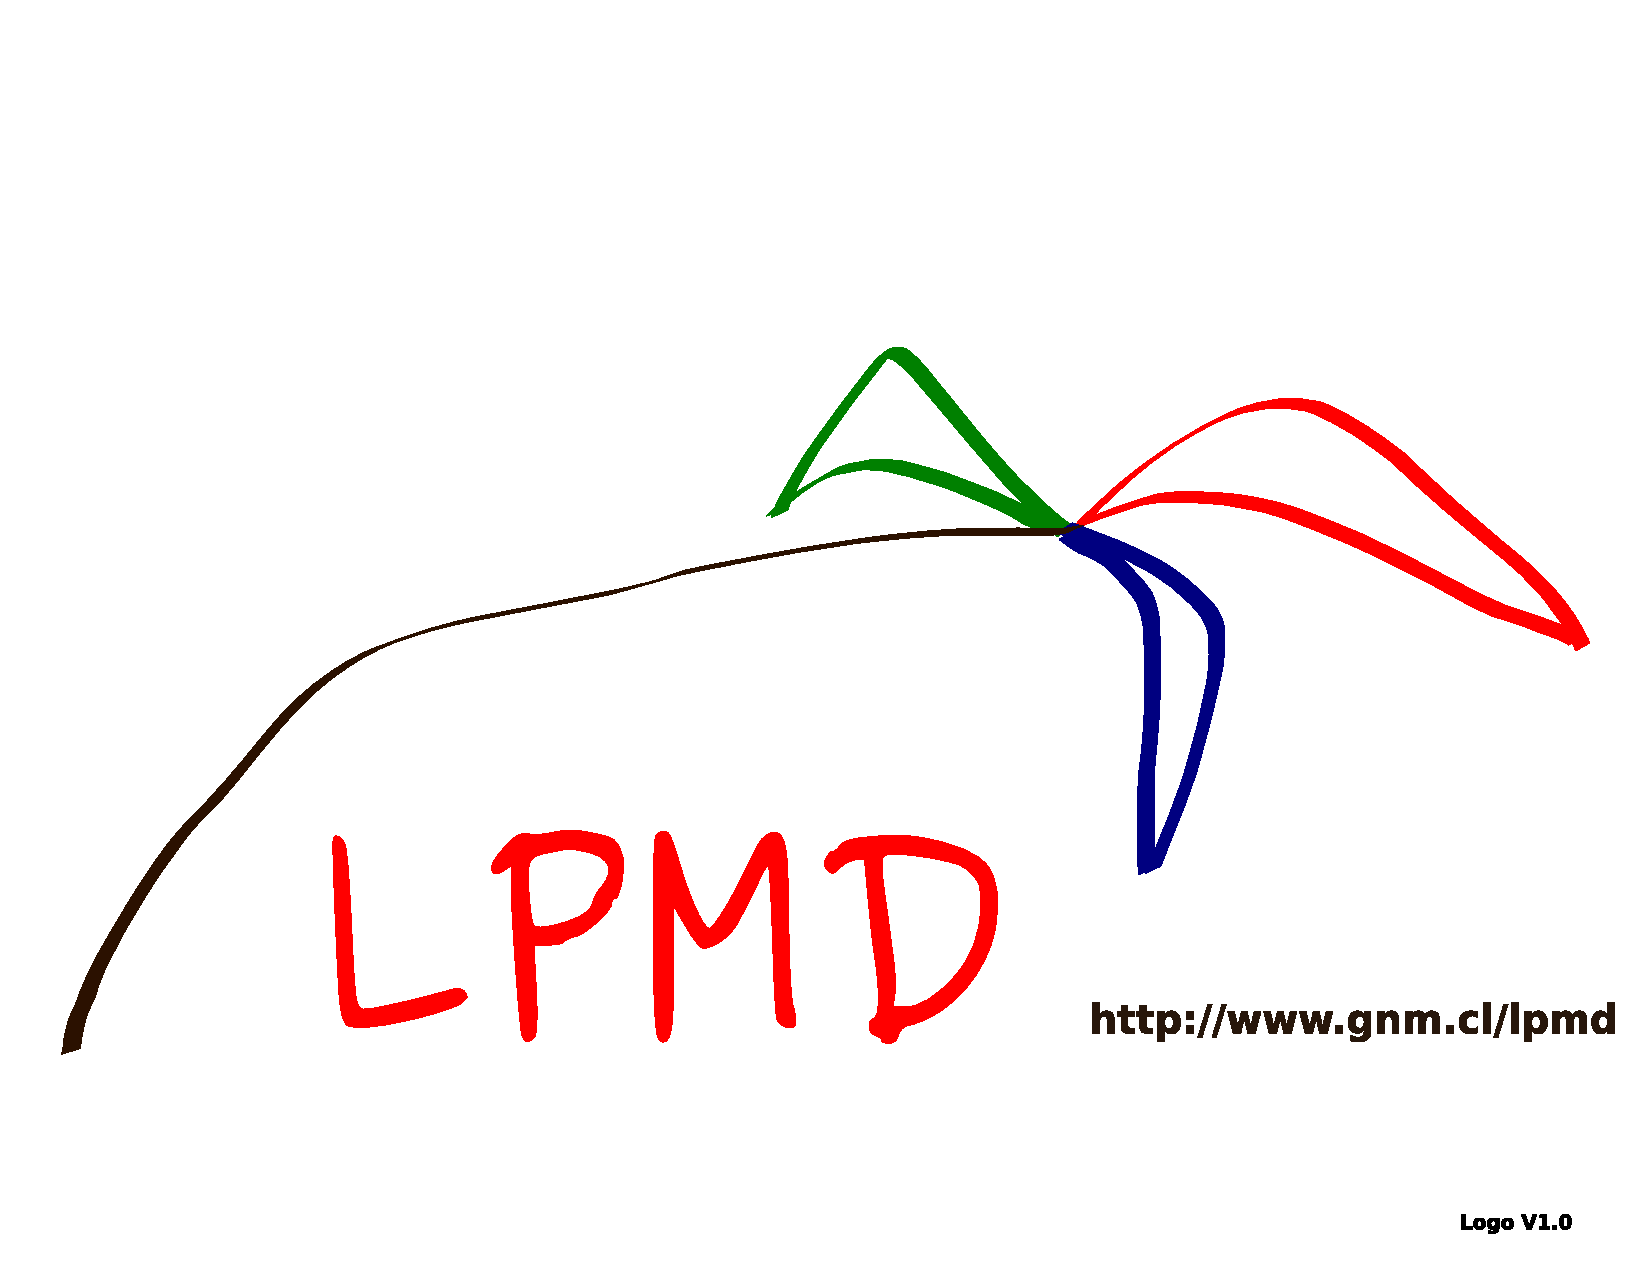
\includegraphics[scale=.35]{logo-lpmd.pdf}}
\title{``Las Palmeras'' Molecular Dynamics - \textbf{LPMD}.}
\maketitle


\tableofcontents
%%%%%%%%%%%%%%%%%%%%%%%%%%%%%%%%%%%%%%%%%%%%%%%%%%%%%%%%%%%%%%%%%%%%%%%%%%%%%%%%%%%%%%%%%%%%%%%%%%%
%%%%%%%%%%%%%%%%%%%%%%%%%%%%%%%%%%%%%%%%%%%%%%%%%%%%%%%%%%%%%%%%%%%%%%%%%%%%%%%%%%%%%%%%%%%%%%%%%%%
\chapter{El Programa}
\label{chap:lpmd}

\section{Or\'igenes.}

El c\'odigo \index{lpmd}{\lpmd} comenz\'o su desarrollo durante junio del a\~no 2007 como una idea de implementar din\'amica molecular de forma modular, tratando de ser lo m\'as amigable para el usuario en el dise\~no de plugins e implementaci\'on de actualizaciones. Los programadores principales de la primera etapa del c\'odigo fueron, \index{Sergio Davis}Sergio Davis, \index{Claudia Loyola}Claudia Loyola y \index{Joaqu\'in Peralta}Joaqu\'in Peralta, todos ellos integrantes del \index{GNM}\textit{Grupo de NanoMateriales} (\textbf{http://www.gnm.cl}). Actualmente existen m\'as colaboradores en el desarollo del c\'odigo~\ref{chap:auth}.

Las versiones que se han lanzado en formato estable son:

\begin{itemize}
 \item Version 0.5.2 : Lanzada 05 de Agosto 2008.
 \item Version 0.5.1 : Lanzada 30 de Abril 2008.
 \item Version 0.5.0 : Lanzada 04 de Abril 2008.
 \item Version 0.4.0 : Lanzada Julio 2007.
\end{itemize}

El sistema de actualizaci\'on va siendo administrado completamente por los desarrolladores. A partir de la versi\'on 0.5 de {\lpmd} se cuenta con tres paquetes principales de desarrollo.

\begin{itemize}
 \item liblpmd \\
\textbf{API} principal de programaci\'on desarrollada por el grupo. Esta \textbf{API} es la columna vertebral de todas las caracter\'isticas que presenta {\lpmd}. Por favor refi\'erase a m\'as caracter\'isticas en el ap\'endice ~\ref{ap:API}
 \item lpmd-plugins \\
Es un set de plugins que han sido implementados, que cuentan con caracter\'isticas provenientes de la \textbf{API}, son en general potenciales interat\'omicos, integradores, analizadores de celdas de simulaci\'on, as\'i como tambi\'en manejadores de archivos de din\'amica molecular.
 \item lpmd \\
{\lpmd} es un software de din\'amica molecular que utiliza plugins implementados por usuarios para realizar todo el trabajo de simulaci\'on. Tambi\'en incluye herramientas como \textbf{lpmd-analyzer} y \textbf{lpmd-converter} que son utilizados para la generaci\'on de configuraciones, as\'i como tambi\'en el an\'alisis a partir de ficheros de simulaci\'on de din\'amica molecular.
\end{itemize}

\section{Idea Principal}

El esquema principal de {\lpmd}, es la utilizaci\'on de un archivo de control (\verb|fichero.control|) el cual es cargado directamente por el ejecutable \verb|lpmd|.

Por ejemplo, consideremos un sistema de din\'amica molecular en el cual todas las opciones, tales como temperatura inicial, pasos de tiempo a simular, integrador, potencial interat\'omico, posiciones at\'omicas, etc. est\'an especificadas en un fichero llamado ``\verb|simulacion.control|'', entonces lpmd puede ejecutarse simplemente con,

\begin{center}
 \texttt{lpmd simulacion.control > simulacion.output}
\end{center}

o tambi\'en podemos utilizar,

\begin{center}
 \texttt{lpmd < simulacion.control > simulacion.output}
\end{center}

De esta forma, {\lpmd} carga toda la informaci\'on necesaria ubicada en el fichero \verb|simulacion.control| y toda la informaci\'on de salida es guardada en el fichero \verb|simulacion.output|. Es importante destacar que {\lpmd} adem\'as interact\'ua y genera archivos de salida seg\'un los m\'odulos que hagan referencia a esos archivos.

\section{Otras Caracter\'isticas}

Otras caracter\'isticas de {\lpmd} es que cuenta con flags para el manejo de variables internas en un fichero de control, por ejemplo, se pueden correr muchos sistemas con distintas temperaturas iniciales. Para ello consideremos, un fichero de control con una sintaxis del tipo,

\begin{verbatim}
 ...
 prepare temperature t=$(TEMP)
 ...
\end{verbatim}

entonces, podemos ejecutar {\lpmd} de la siguiente forma para asignar a \verb|TEMP| un \'unico valor real, dado directamente por l\'inea de comandos, por ejemplo:

\begin{center}
 \texttt{lpmd -o TEMP=500 simulacion.control > simulacion.output}
\end{center}

de esta forma el programa comienza la simulaci\'on del sistema con una temperatura inicial de 500K. 

Una de las ventajas de una caracter\'istica como \'esta es que reduce mucho la dificultad de implementar scripts para distintas simulaciones o simulaciones consecutivas de din\'amica molecular. Por ejemplo con un solo comando podemos correr un set de simulaciones con un valor distinto asociado a una variable del archivo de control. Para el caso de la temperatura:

\begin{center}
 \texttt{for i in 300 400 500 ; \\do lpmd -o TEMP=\$i simulacion.control > simulacion-\$i.output ; done}
\end{center}

realiza tres simulaciones seguidas con diferentes temperaturas iniciales con un solo fichero de control.


Otro de los flags importantes de {\lpmd} es \verb|-p| que brinda informaci\'on acerca de los plugins que se encuentran instalados en el sistema y que identifica directamente {\lpmd}. Pruebe por ejemplo algo como :

\begin{center}
 \texttt{lpmd -p angdist}
\end{center}

donde \verb|angdist| corresponde al plugin que calcula la distribuci\'on angular de una celda de simulaci\'on. Para m\'as opciones vea \verb|lpmd -h| o \verb|man lpmd|. En los cap\'itulos siguientes se dar\'a una descripci\'on mucho m\'as detallada de otras caracter\'isticas {\lpmd} y sus funcionalidades.
%%%%%%%%%%%%%%%%%%%%%%%%%%%%%%%

%%%%%%%%%%%%%%%%%%%%%%%%%%%%%%%%%%%%%%%%%%%%%%%%%%%%%%%%%%%%%%%%%%%%%%%%%%
%%%%%%%%%%%%%%%%%%%%%%%%%%%%%%%%%%%%%%%%%%%%%%%%%%%%%%%%%%%%%%%%%%%%%%%%%%%%%%%%%%%%%%%%%%%%%%%%%%%%%%%%%
%CAPITULO 2%%%%%%%%%%%%%%%%%%%%%%%%%%%%%%%%%%%%%%%%%%%%%%%%%%%%%%%%%%%%%%%%%%%%%%%%%%%%%%%%%%%%%%%%%%%%%%
%%%%%%%%%%%%%%%%%%%%%%%%%%%%%%%%%%%%%%%%%%%%%%%%%%%%%%%%%%%%%%%%%%%%%%%%%%%%%%%%%%%%%%%%%%%%%%%%%%%%%%%%%
%%%%%%%%%%%%%%%%%%%%%%%%%%%%%%%%%%%%%%%%%%%%%%%%%%%%%%%%%%%%%%%%%%%%%%%%%%%%%%%%%%%%%%%%%%%%%%%%%%%%%%%%%
\chapter{Instalaci\'on}
\label{chap:inst}

{\lpmd} ha sido probado en distintas arquitecturas y compiladores. Sin embargo a partir de la version 0.6.0 s\'olo hemos mantenido pruebas sobre dos arquitecturas principales :

\begin{itemize}
 \item Linux I686/AMD64
 \item OS/X
\end{itemize}

Adem\'as actualmente {\lpmd} cuenta con \verb|lpmd-installer|, un programa enfocado a la instalaci\'on sencilla de lpmd en cualquier maquina, que est\'a escrito en python. Nosotros recomendamos a los usuarios no expertos que utilizen \verb|lpmd-installer| para la instalaci\'on de {\lpmd} en sus sistemas.

\section{lpmd-installer}

Utilidad enfocada para una instalación amigable de {\lpmd}, llamada \verb|lpmd-installer|. Este programa escrito en python se encarga de instalar de forma automatica los 3 paquetes principales que forman parte de lpmd. Estos son :

\begin{itemize}
 \item liblpmd : API principal del proyecto
 \item plugins : Set de plugins para din\'amica molecular y an\'alisis de estructuras.
 \item lpmd : Programa principal, con utilitarios.
\end{itemize}

\fb{
\begin{minipage}[l]{10cm}
Si no se desea utilizar la versi\'on autom\'atica de instalaci\'on basada en \texttt{lpmd-installer} contin\'ue a la siguiente secci\'on.
\end{minipage}
}

\subsection{Instalando lpmd-installer}

El programa \verb|lpmd-installer| es un script escrito en python por lo que las formas de instalaci\'on son bastantes simples, para funcionar correctamente \verb|lpmd-installer| necesita :

\begin{itemize}
\item Python 2.3 o superior.
\item Conecci\'on a internet.
\end{itemize}

Para instalar \verb|lpmd-installer| en su sistema existen dos formas, la primera es para distribuciones basadas en debian en donde contamos con un repositorio especial para ello, o bien en otro tipo de distribuciones para lo cual es necesario descargar el programa e instalarlo manualmente.

\subsubsection{Distribuciones basadas en Debian}

Se ha probado en distribuciones como Debian/Ubuntu, para proceder, en primer lugar como administrador, edite el fichero \verb|\etc\apt\sources.list| y a\~nada :

\begin{verbatim}
 #GNM Repositories
 deb http://www.gnm.cl/repos ./
\end{verbatim}

Luego, como administrador nuevamente, ejecute :

\begin{verbatim}
 apt-get update
 apt-get install lpmd-installer
\end{verbatim}

Ahora verifique que tenga el comando
\begin{verbatim}
 username@machine:~$ lpmd-installer 
 lpmd-installer [ -i <branch or version> | -u ] [-v] [-p <prefix>] [-P <package>] 
                [-s <server>] [-S <suffix>] [ -d <sources dir>] [-t]
 username@machine:~$
\end{verbatim}

Listo ya esta en condiciones de poder instalar {\lpmd} facilmente.

\subsubsection{Otras Distribuciones}

Para instalar \verb|lpmd-installer| en distribuciones no basadas en Debian, es necesario descargar el programa directamente desde internet, puede encontrarlo en esta direcci\'on :

\begin{verbatim}
 http://www.gnm.cl/lpmd/uploads/Main/lpmd-installer
\end{verbatim}

Descarge el archivo y asignele permisos de ejecuci\'on :

\begin{verbatim}
 chmod 755 lpmd-installer
\end{verbatim}

Luego de eso, se puede copiar o mover a algun lugar donde se tenga \verb|PATH| del sistema. En la mayor\'ia de los sistemas *nix puede copiarse o moverse a :

\begin{verbatim}
 cp lpmd-installer /usr/local/bin/
\end{verbatim}

Y listo, ahora verifique que tiene el comando \verb|lpmd-installer| disponible en su sistema.
\begin{verbatim}
 username@machine:~$ lpmd-installer 
 lpmd-installer [ -i <branch or version> | -u ] [-v] [-p <prefix>] [-P <package>] 
                [-s <server>] [-S <suffix>] [ -d <sources dir>] [-t]
 username@machine:~$
\end{verbatim}

\subsection{Probando lpmd-installer}
El programa cuenta con todo lo necesario para instalar {\lpmd} en un sistema o en cuentas personales, as\'i como tambi\'en facilidades para instalar \textit{plugins} externos, tales como \verb|lpvisual|. Entre las opciones principales de \verb|lpmd-installer| se cuenta con :

\begin{itemize}
 \item \verb|-l| : Lista las versiones disponibles de instalar asociadas al paquete.
 \item \verb|-p| : Especifica donde se instalar\'a.
 \item \verb|-P| : Especif\'ica que paquete se instalar\'a.
 \item \verb|-d| : Especif\'ica donde quedar\'an los sources, sino se especif\'ica estos son elmiminados despu''es de la instalaci\'on.
 \item \verb|-u| : Actualiza la versi\'on de {\lpmd} que se encuentra en su sistema.
\end{itemize}

A continuaci\'on veremos como se instala {\lpmd} utilizando \verb|lpmd-installer|.

\subsection{Instalando lpmd en el sistema}

Antes de ejecutar la instalaci\'on directa de {\lpmd} en el sistema es conveniente ver la disponibilidad de las versiones disponibles en el servidor principal, para ello ejecute \verb|lpmd-installer -l|, y obtendra una lista como la siguiente :

\begin{verbatim}
username@machine:~$ lpmd-installer -l
These are the available versions of package lpmd:

From branch 0.5: 
    0.5.4-delta2
    0.5.4-delta2-openmp
    0.5.4-delta1
    0.5.4
    0.5.3

From branch 0.6: 
    0.6.1
    0.6.0
username@machine:~$
\end{verbatim}

Elegimos de la lista la version que se desea instalar, en este caso la version 0.6.1, si intentamos instalar esta version en el sistema sin ser \textbf{administrador} obtendremos un mensaje como  :

\begin{verbatim}
username@machine:~$ lpmd-installer -i 0.6.1
Preparing to install lpmd 0.6.1
[Error] You do not have permission to install on /usr/local
username@machine:~$
\end{verbatim}

Esto ocurre debido a que, por defecto, lpmd se intenta instalar en \verb|/usr/local| y un usuario normal no tiene permisos de escritura en este directorio. La manera correcta de proceder es, instalarlo como \textbf{administrador}. Para ello :

\begin{verbatim}
username@machine:~$ sudo -s
[sudo] password for username: 
root@machine:~# lpmd-installer -i 0.6.1
\end{verbatim}

Ahora si, el proceso comenzar\'a de forma autom\'atica a descargar desde el servidor principal los paquetes necesarios para la instalaci\'on. Recuerde que se requiere al menos un compilador de \verb|C++| para llevar a cabo la instalaci\'on. Tambien es recomendable contar con las librer\'ias \verb|zlib|, en la manyor\'ia de los sistemas es un paquete con el nombre \verb|zlib1g-dev|, que en distribuci\'ones basadas en Debian ser\'ia :

\begin{verbatim}
username@machine:~$ sudo -s
[sudo] password for username: 
root@machine:~# apt-get installl zlib1g-dev
\end{verbatim}


\subsection{Instalando lpvisual utilizando lpmd-installer}

Con \verb|lpmd-installer| tambi\'en podremos realizar la instalaci\'on de \verb|lpvisual| un plugin independiente basado en OpenGL para la visualizaci\'on de configuraciones at\'omicas de distintos tipos. Para la correcta compilaci\'on del c\'odigo fuente es necesario tener instaladas las librerias principales del proyecto OpenGL, para ello, en distribuciones basadas en Debian se puede utilizar :

\begin{verbatim}
username@machine:~$ sudo -s
[sudo] password for username: 
root@machine:~# apt-get install libglut3-dev
\end{verbatim}

Ahora, para instalar facilmente lpvisual en el sistema podemos utilizar las mismas opciones de \verb|lpmd-installer| utilizadas previamente :

\begin{verbatim}
username@machine:~$ lpmd-installer -P lpvisual -l
These are the available versions of package lpvisual:

From branch 2.0: 
    6.0
username@machine:~$  
\end{verbatim}

Entonces elegimos la version de \verb|lpvisual| que deseamos instalar y la instalamos facilmente con :

\begin{verbatim}
username@machine:~$ lpmd-installer -P lpvisual -i 6.0
....
\end{verbatim}

Con esto entonces hemos instalado un \textbf{plugin adicional} utilizando lpmd-installer.

\subsection{Instalando lpmd en una cuenta personal}

Si no somos administradores o no tenemos acceso a \'el es posible que nuestra intenci\'on sea instalar {\lpmd} en una cuenta personal, para ello \verb|lpmd-installer| cuenta con flags opcionales para especificar  esto. Consideremos que deseamos instalar {\lpmd} en un directorio \verb|~/local/| para ello es necesario entonces especificar el directorio con el flag \verb|-p| como se muestra a continuaci\'on :

\begin{verbatim}
username@machine:~$ lpmd-installer -i 0.6.1 -p /home/username/local
....
username@machine:~$
\end{verbatim}

con este comando hemos instalado entonces {\lpmd} en nuestra cuenta personal, adem\'mas podemos elegir mantener el c\'odigo fuente en algun directorio en especial :

\begin{verbatim}
username@machine:~$ lpmd-installer -i 0.6.1 -p /home/username/local -d /home/username/sources
....
username@machine:~$
\end{verbatim}

Para m\'as soporte y ayuda puede enviar e-mail a los desarrolladores o visitar la web principal del proyecto \verb|http://www.gnm.cl|.

\section{Descarga}

Si ha decidido no instalar {\lpmd} utilizando \verb|lpmd-installer| entonces debe descargar los 3 paquetes principales para la posterior instalaci\'on, para ello existen dos versiones disponibles, la version estable y la versi\'on de pruebas. En ambos casos se deben descargar los tres paquetes principales asociados a {\lpmd}, \verb|API| (libreria principal), \verb|plugins| (m\'odulos y complementos) y \verb|lpmd| (ejecutables y utilitarios).

%%%%%%%%%%%%%%%%%%%%%%%%%%%%%%%%%%%%%%%%%%%%%%%%%%%%%%%%%%%%%%%%%
%%%%%%%%%%%%%%%%%%%%%%%%%%%%%%%%%%%%%%%%%%%%%%%%%%%%%%%%%%%%%%%%%
\subsection{Descarga de versi\'on estable}

La \'ultima versi\'on estable de los paquetes es :

\begin{itemize}
 \item liblpmd : ver. 0.2.1
 \item plugins : ver. 0.2.1
 \item lpmd    : ver. 0.6.1
\end{itemize}

Estos pueden ser descargados directamente en la pagina web \texttt{http://www.gnm.cl/lpmd}, o bien solicitados por e-mail.

%%%%%%%%%%%%%%%%%%%%%%%%%%%%%%%%%%%%%%%%%%%%%%%%%%%%%%%%%%%%%%%%%
%%%%%%%%%%%%%%%%%%%%%%%%%%%%%%%%%%%%%%%%%%%%%%%%%%%%%%%%%%%%%%%%%
\subsection{Descarga de versi\'on en desarrollo}

Para los interesados en el desarrollo de {\lpmd} y sus complementos principales(API, plugins, utilitarios, etc.), la version de pruebas ``\textit{testing}'' se puede descargar con subversion, esta es la forma principal que utilizan los desarrolladores del c\'odigo, si se desea tener los \'ultimos \textit{updates} es la forma m\'as recomendable :

\begin{center}
 \begin{verbatim}
  svn co svn://www.gnm.cl/lpmd/liblpmd/testing liblpmd-uns
  svn co svn://www.gnm.cl/lpmd/plugins/testing plugins-uns
  svn co svn://www.gnm.cl/lpmd/lpmd/testing lpmd-uns
 \end{verbatim}
\end{center}

Est\'a disponible adem\'as una rama \verb|unstable|; sin embargo, no recomendamos utilizarla para c\'alculos de Din\'amica Molecular. S\'olo utilizable para investigaci\'on y prueba de c\'odigos.

\section{Instalaci\'on}

Para un correcto procedimiento de instalaci\'on es necesario instalar en primer lugar la \verb|API| del proyecto antes de cualquier otro paquete. El orden de las instalaciones posteriores no es importante.

\fb{
\begin{minipage}[l]{10cm}
Nota : Los que poseen la versi\'on testing/unstable cuentan con \texttt{NMC} (\textit{NanoMaterialsConfigure}) una utilidad desarrollada por Sergio Davis en python, similar al ya conocido \texttt{configure} de GNU pero mucho m\'as ajustado a nuestros requerimientos.
\end{minipage}
}

%%%%%%%%%%%%%%%%%%%%%%%%%%%%%%%%%%%%%%%%%%%%%%%%%%%%%%%%%%%%%%%%%
%%%%%%%%%%%%%%%%%%%%%%%%%%%%%%%%%%%%%%%%%%%%%%%%%%%%%%%%%%%%%%%%%
\subsection{Instalando API liblpmd}

En primer lugar descomprima el paquete de la \textbf{liblpmd},

\control{tar -xvzf liblpmd-X.X.X.tar.gz}

lo que le generar\'a un nuevo directorio; para instalar esta librer\'ia con todos los requerimientos necesarios para el funcionamiento de {\lpmd} y la implementaci\'on de plugins ejecute :

\control{./setup \\ make}

y como administrador,

\control{make install}

Por \textit{default} el directorio de instalaci\'on de la API es \verb|/usr/local/|, en caso de requerir una ubicaci\'on distinta revise las opciones con \verb|./setup --help|. Y si desea instalarlo en un directorio personal refi\'erase a la secci\'on~\ref{subsub:personaldir}.

En caso de cualquier error en el proceso de instalaci\'on env\'ie un e-mail a alguno de los desarrolladores principales o en su defecto a \verb|gnm@gnm.cl|.

%%%%%%%%%%%%%%%%%%%%%%%%%%%%%%%%%%%%%%%%%%%%%%%%%%%%%%%%%%%%%%%%%
%%%%%%%%%%%%%%%%%%%%%%%%%%%%%%%%%%%%%%%%%%%%%%%%%%%%%%%%%%%%%%%%%
\subsection{Instalando plugins}

Uno de los requerimientos b\'asicos de {\lpmd} es tener bien especificada la ubicaci\'on de los plugins que {\lpmd} requiere, para el caso de que requiera instalar lpmd en un lugar distinto al que viene por \textit{default}, refierase a la secci\'on~\ref{subsub:personaldir}. Si continuará con el desarrollo standard de instalaci\'on entonces puede configurar y compilar el paquete de plugins utilizando :

\control{./setup  \\ make}

y proceder la instalaci\'on como administrador:

\control{make install}

Esto ubicar\'a todos los plugins incluidos en el paquete \verb|plugins| en el directorio \verb|/usr/local/lib/lpmd| (si se instalo en la ubicaci\'on por \textit{default}). De esta forma ya estamos listos para comenzar la instalaci\'on de lpmd y realizar las primeras pruebas.

%%%%%%%%%%%%%%%%%%%%%%%%%%%%%%%%%%%%%%%%%%%%%%%%%%%%%%%%%%%%%%%%%
%%%%%%%%%%%%%%%%%%%%%%%%%%%%%%%%%%%%%%%%%%%%%%%%%%%%%%%%%%%%%%%%%
\subsection{Instalando lpmd}

Es uno de los paquetes m\'as peque\~nos y r\'apidos de instalar; para proceder, se hace de manera similar que los anteriores, ejecutando:

\control{./setup \\ make}

y proceder a instalar como administrador:

\control{make install}

Esto generar\'a un set de ejecutables \verb|lpmd|, \verb|lpmd-analyzer|, \verb|lpmd-converter| y \verb|lpmd-visualizer| en \verb|/usr/local/bin/|, que puede ser ejecutado desde cualquier sitio (si se presenta alg\'un problema, corriga su \verb|PATH|).

Puede correr lpmd con

\begin{verbatim}
username@machine:~$ lpmd
...
LPMD version 0.6.1
Using liblpmd version 2.0.1

Usage: lpmd [--verbose | -v ] [--lengths | -L <a,b,c>] [--angles | 
-A <alpha,beta,gamma>] [--vector | -V <ax,ay,az,bx,by,bz,cx,cy,cz>] 
[--scale | -S <value>] [--option | -O <option=value,option=value,...>] 
[--input | -i plugin:opt1,opt2,...] [--output | -o plugin:opt1,opt2,...] 
[--use | -u plugin:opt1,opt2,...] [--replace-cell | -r] [file.control]
       lpmd [--pluginhelp | -p <pluginname>]
       lpmd [--help | -h]
\end{verbatim}

\subsection{Problemas t\'ipicos post-instalaci\'on}

\subsubsection{Error cargando librer\'ia}

Es uno de los errores m\'as comunes en la rama 0.5.X de {\lpmd}, luego de la instlaci\'on de {\lpmd}. Ocurre que al ejecutar {\lpmd} no muestra nada m\'as que un error referencial a la librer\'ia liblpmd que no puede ser encontrada.

La forma de corregir el problema es,

\begin{itemize}
 \item Editar /etc/ld.so.conf
 \item A\~nadir al archivo la l\'inea /usr/local/lib (o donde se haya instalado liblpmd)
 \item Ejecutar como admininistrador el comando: ldconfig
\end{itemize}

Ahora deber\'ia ejecutar el comando sin problemas.

\subsection{Instalaci\'on de lpmd en directorio personal}
\label{subsub:personaldir}

Podemos instalar cada uno de los paquetes (\textbf{liblpmd}, \textbf{plugins} y \textbf{lpmd}) en un directorio personal, para eso consideremos un ejemplo, en el cual deseamos instalar estos paquetes en el directorio \verb|local| ubicado en el \textit{home} del usuario, el procedimiento ser\'ia:

\begin{itemize}
 \item Para liblpmd
 \begin{verbatim}
 ./setup --prefix=/home/user/local
 make
 make install
 \end{verbatim}
 \item Para plugins
 \begin{verbatim}
 ./setup --prefix=/home/user/local
 make
 make install
 \end{verbatim}
 \item Para lpmd, es necesario indicar con variables de ambiente para la compilaci\'on, note que \verb|\\| indica que es una sola l\'inea que contin\'ua.
 \begin{verbatim}
 ./setup --prefix=/home/user/local
 make
 make install
 \end{verbatim}
\end{itemize}

De esta forma se generar\'an los esqueletos en \verb|/home/user/local| con \verb|bin|, \verb|lib|, etc. Ahora puede ejecutarlos si su \verb|PATH| esta bien configurado a la direcci\'on \verb|/home/user/local/bin|.


%%%%%%%%%%%%%%%%%%%%%%%%%%%%%%%%%%%%%%%%%%%%%%%%%%%%%%%%%%%%%%%%%
%%%%%%%%%%%%%%%%%%%%%%%%%%%%%%%%%%%%%%%%%%%%%%%%%%%%%%%%%%%%%%%%%
\subsection{Actualizando lpmd}

 Actualmente {\lpmd} solo puede ser actualizado utilizando el paquete \verb|lpmd-installer| o bien si es desarrollador, utilizando subversion. Recomendames que s\'olo utilize estos m\'etodos de actualizaci\'on.

%%%%%%%%%%%%%%%%%%%%%%%%%%%%%%%%%%%%%%%%%%%%%%%%%%%%%%%%%%%%%%%%%%%%%%%%%%%%%%%%%%%%%%%%%%%%%%%%%%%%%%%%%
%%%%%%%%%%%%%%%%%%%%%%%%%%%%%%%%%%%%%%%%%%%%%%%%%%%%%%%%%%%%%%%%%%%%%%%%%%%%%%%%%%%%%%%%%%%%%%%%%%%%%%%%%
%CAPITULO 3%%%%%%%%%%%%%%%%%%%%%%%%%%%%%%%%%%%%%%%%%%%%%%%%%%%%%%%%%%%%%%%%%%%%%%%%%%%%%%%%%%%%%%%%%%%%%%
%%%%%%%%%%%%%%%%%%%%%%%%%%%%%%%%%%%%%%%%%%%%%%%%%%%%%%%%%%%%%%%%%%%%%%%%%%%%%%%%%%%%%%%%%%%%%%%%%%%%%%%%%
%%%%%%%%%%%%%%%%%%%%%%%%%%%%%%%%%%%%%%%%%%%%%%%%%%%%%%%%%%%%%%%%%%%%%%%%%%%%%%%%%%%%%%%%%%%%%%%%%%%%%%%%%
\chapter{El Fichero de Control}
\label{chap:input}

Una de las piezas fundamentales en {\lpmd} para la corrida de una simulaci\'on molecular son los ficheros iniciales de configuraci\'on del sistema. Para el correcto funcionamiento se necesita un fichero de control, este fichero espec\'ifica casi la totalidad de los requerimientos de la simulaci\'on y en ocasiones el 100\%. Aunque en la mayor\'ia de los casos se requiere un fichero adicional en donde se encuentran las posiciones at\'omicas de los \'atomos pertenecientes a la celda de simulaci\'on. Es por eso que en primer lugar, antes de revisar el fichero de control, revisaremos de forma general los archivos de posiciones at\'omicas.

\section{Fichero con Posiciones At\'omicas}

{\lpmd} puede manejar los tipos de fichero de posiciones at\'omicas seg\'un los m\'odulos de los que se disponga; actualmente \textbf{lpmd-plugins} cuenta con varios m\'odulos de formatos de ficheros para especificar las posiciones at\'omicas, entre ellos \textbf{xyz}, \textbf{lpmd}, \textbf{dlpoly} (archivos \verb|CONFIG| o \verb|HISTORY| de dl\_poly), etc.

Esperamos que los usuarios, seg\'un su necesidad, ayuden a implementar o solicitar a los desarrolladores tipos espec\'ificos de sistemas de posiciones at\'omicas para din\'amica molecular. Veamos brevemente en que consisten algunos de ellos. Para informaci\'on espec\'ifica de cada m\'odulo, vea la secci\'on~\ref{chap:modulos:entradasalida}.

%%%%%%%%%%%%%%%%%%%%%%%%%%%%%%%%%%%%%%%%%%%%%%%%%%%%%%%%%%%%%%%%%
%%%%%%%%%%%%%%%%%%%%%%%%%%%%%%%%%%%%%%%%%%%%%%%%%%%%%%%%%%%%%%%%%
\subsection{Fichero .xyz}

Es el est\'andar de ficheros \verb|xyz| utilizado en muchos c\'odigos de simulaci\'on computacional, es un archivo simple que cuenta con la informaci\'on de las posiciones at\'omicas del sistema en cordenadas cartesianas y sus unidades en \AA. La estructura de un fichero es :
\begin{center}
\begin{tabular}{l|l}
 \verb|N| & Especifica el n\'umero de \'atomos en la celda \\
 \verb|comment| & Una l\'inea adicional de comentario, t\'itulo, etc. \\
 \verb|Sym X Y Z| & S\'imbolo at\'omico y las posiciones en coordenadas cartesianas. \\
\end{tabular}
\end{center}

Actualmente el m\'odulo \verb|xyz| soporta tres niveles distintos estos son 0,1 y 2 los que indican la informaci\'on que poseen los \'atomos an cada l\'inea. El nivel cero indica las posiciones at\'omicas, el nivel uno a\~nade las velocidades y el nivel 2 las aceleraciones. Es decir :

\begin{itemize}
\item 0 : \verb|Sym X Y Z| (valor por defecto).
\item 1 : \verb|Sym X Y Z VX VY VZ|.
\item 2 : \verb|Sym X Y Z VX VY VZ AX AY AZ|.
\end{itemize}

Cualquiera de estos niveles puede ser le\'ido como un fichero de entrada para el formato \verb|xyz|.

%%%%%%%%%%%%%%%%%%%%%%%%%%%%%%%%%%%%%%%%%%%%%%%%%%%%%%%%%%%%%%%%%
%%%%%%%%%%%%%%%%%%%%%%%%%%%%%%%%%%%%%%%%%%%%%%%%%%%%%%%%%%%%%%%%%
\subsection{Fichero .lpmd}

A partir de {\lpmd} 0.6.0, existe un nuevo formato 2.0 para los ficheros \verb|.lpmd| (compatible con la versi\'on 1.0). Este es un fichero con las posiciones escaladas de los \'atomos que forman la celda. Es de tipo ASCII y su estructura principal est\'a dada por:

\begin{center}
 \begin{tabular}{l|l}
 \verb|LPMD VERSION X.X | & Especifica la versi\'on del fichero \verb|.lpmd| \\
 \verb|HEAD X Y Z| & Especif\'ica la informaci\'on que posee cada l\'inea at\'omica. \\
 \verb|cell properties | & Propiedades de la celda, pueden ser 3 vectores o longitudes y \'angulos. \\
 \verb|Sym sx sy sz| & S\'imbolo at\'omico y las posiciones escaladas en cada eje [0,1].\\
\end{tabular}
\end{center}

Al igual que el \verb|xyz|, los ficheros de tipos \verb|lpmd| cuentan con niveles (0,1 y 2) junto con flags extras tales como color del \'atomo o alguna propiedad que se puede o no guardar, seg\'un los requerimientos del mismo usuario.

%%%%%%%%%%%%%%%%%%%%%%%%%%%%%%%%%%%%%%%%%%%%%%%%%%%%%%%%%%%%%%%%%
%%%%%%%%%%%%%%%%%%%%%%%%%%%%%%%%%%%%%%%%%%%%%%%%%%%%%%%%%%%%%%%%%
\subsection{Otros Formatos Soportados}

Pese a que los formatos principales de entrada recomendados son \textbf{xyz} y \textbf{lpmd}, existen actualmente otros formatos que son soportados para lectura/escritura de configuraciones at\'omicas, algunos de ellos son listados en la tabla~\ref{tab:modinout}. Si tiene dudas con respecto a alg\'un formato, as\'i como sugerencias o requerimientos, no dude en contactarnos.

\section{El Fichero de configuraci\'on .control}

Es el fichero principal para realizar la simulaci\'on computacional. Es por eso que en primer lugar se har\'a una descripci\'on general de cada una de sus partes principales y luego veremos \'estas de forma mucho m\'as detallada.


Entre los puntos generales a considerar en un fichero de control, est\'an:

\begin{itemize}
 \item \# Es una l\'inea de comentario. (Evitelas dentro de un bloque \texttt{use ... enduse}).
 \item Pese a que puede ser aleatorio el orden de los flags, se recomienda llevar un orden.
 \item Recomendamos \textbf{definir los m\'odulos} antes de utilizarlos. Tampoco es obligaci\'on.
 \item Existen m\'odulos en un fichero de control que \textbf{no} pueden ser omitidos, como por ejemplo, un \textbf{cellmanager}. Sin embargo la mayor\'ia de estos casos, pueden ser entregados por l\'inea de comando.
\end{itemize}

Con estos puntos previos en mente, veamos entonces cuales son las secciones principales a tener en cuenta dentro de un \textbf{fichero de control} para utilizar con {\lpmd}, consideremos de forma general el esquema que se muestra a continuaci\'on.

\fb{ 
\texttt{
\begin{tabular}{lcl}
 \#Cell Properties & $\rightarrow$ & Propiedades de la celda.\\
 cell ... &&\\
 \#Input/Output & $\rightarrow$ & Principales ficheros de entrada y salida\\
 input ... &&\\
 output ... &&\\
 \#General & $\rightarrow$ & Setting generales de la simulaci\'on\\
 prepare ... &&\\
 steps ... &&\\
 monitor ... &&\\
 \#Filters & $\rightarrow$ & Filtros a aplicar sobre la muestra.\\
 filter ... &&\\
 \#Module Load & $\rightarrow$ & Carga de todos los modulos necesarios.\\
 use ... &&\\
 enduse ... &&\\
 \#Module Apply & $\rightarrow$ & Indica como son aplicados los modulos.\\
 apply ... &&\\
 potential ... &&\\
 integrator ... &&\\
\end{tabular}
}
}

Esta entonces es una \textbf{aproximaci\'on general} a los ficheros de entrada utilizados en din\'amica molecular por {\lpmd}. Con esta idea en mente veremos a continuaci\'on cada una de las secciones principales del fichero de control.

%%%%%%%%%%%%%%%%%%%%%%%%%%%%%%%%%%%%%%%%%%%%%%%%%%%%%%%%%%%%%%%%%
%%%%%%%%%%%%%%%%%%%%%%%%%%%%%%%%%%%%%%%%%%%%%%%%%%%%%%%%%%%%%%%%%
\subsection{Celda de Simulaci\'on.}

Es la propiedad que describe la celda de simulaci\'on. Es decir el detalle completo de cada uno de los ejes que la conforman, los que pueden ser entregados en forma detallada o en forma general. A continuaci\'on se describir\'a la forma en la cu\'al se entrega \'esta propiedad, que \textit{casi siempre} debe estar presente en el fichero .control y va al comienzo de \'este.

\subsubsection{cell}

El flag cell es utilizado para describir la celda de simulaci\'on y asignar las propiedades de \'esta. Generalmente una celda de simulaci\'on puede venir descrita ya en el formato del fichero de entrada (como es el caso de lo ficheros \texttt{lpmd} o \texttt{CONFIG}). Sin embargo, hay formatos, como el \texttt{xyz}, que no poseen la descripci\'on de la celda, es por eso que es necesario en algunos casos utilizar esta opci\'on. Si se desea dar la opci\'on \verb|cell| aunque la informaci\'on se encuentre en un archivo, \'esta predominar\'a sobre la del archivo.

\begin{itemize} 
\item{Forma 1}

Se utilizan la longitud de los lados y \'angulos de la celda, como sigue:

\control{cell a=10 b=5 c=5 alpha=45 beta=90 gamma=90}

donde,

\fb{ 
\begin{tabular}{lcl}
 a & = & indica el largo de la celda en \textbf{a}.\\
 b & = & indica el largo de la celda en \textbf{b}.\\
 c & = & indica el largo de la celda en \textbf{c}.\\
 alpha & = & indica el \'angulo $\alpha$.\\
 beta & = & indica el \'angulo $\beta$.\\
 gamma & = & indica el \'angulo $\gamma$.\\
\end{tabular}
}

\item{Forma 2}

Se utilizan los 3 vectores bases, poni\'endolos de la siguiente manera en el fichero, note que \verb|\| indican la continuaci\'on de una l\'inea \'unica.

\control{cell ax=1.0 ay=0.0 az=0.0 bx=0.0 by=1.0 bz=0.0 \textbackslash \\cx=0.0 cy=0.0 cz=1.0}

donde: a${i}$, b${i}$ y c${i}$ con $i$={$x$,$y$,$z$} son las coordenadas $x, y$ y $z$ de los vectores bases.

Las posibles formas de ingresar una descripcion de la llamada \verb|cell| pueden ser entregadas como argumentos en la ejecuci\'on de {\lpmd} y no necesitan estar dentro del fichero de \textbf{control}, lo que ayuda a la creaci\'on de \textit{scripts}.

\fb{\begin{minipage}[l]{9.5cm}\tt lpmd -L a,b,c -A alpha,beta,gamma archivo.control \\ lpmd -V ax,ay,az,bx,by,bz,cx,cy,cz archivo.control\end{minipage}}


\item{Forma 3}

Existe una forma extra para celdas cubicas que ahorran un poco la escritura completa de cada t\'ermino de la celda, por ejemplo una celda cubica de largo 5\AA, se puede asignar facilmente con :

\control{cell cubic a=5}

\end{itemize}

\subsubsection{Omitiendo cell}
Como se mencion\'o previamente, hay ocaciones en que el archivo de posiciones at\'omicas posee adem\'as la informaci\'on de la celda de simulaci\'on, para estos casos hay dos formas de \textbf{especificar} a {\lpmd} que debe leer la informaci\'on desde ese archivo.

\begin{itemize} 
\item{Forma 1}

Se utilizan opciones especiales dentro del mismo fichero de control :

\control{set replacecell true}

\item{Forma 2}

Se especifica en la ejecuci\'on misma de lpmd con el flag \verb|-r|.

\fb{\begin{minipage}[l]{9.5cm}\tt lpmd archivo.control -r\end{minipage}}

\end{itemize}

%%%%%%%%%%%%%%%%%%%%%%%%%%%%%%%%%%%%%%%%%%%%%%%%%%%%%%%%%%%%%%%%%
%%%%%%%%%%%%%%%%%%%%%%%%%%%%%%%%%%%%%%%%%%%%%%%%%%%%%%%%%%%%%%%%%
\subsection{Entrada - Salida}

\subsubsection{input}

Existen actualmente dos formas de ingreso de un sistema de entrada para la configuraci\'on at\'omica que se requiere simular; estas son, el ingreso de las posiciones at\'omicas de la celda a trav\'es de un archivo (por ejemplo \verb|.xyz| o \verb|.lpmd|) y el otro es mediante m\'odulos que generan autom\'aticamente celdas at\'omicas con ciertas propiedades, por ejemplo celdas \textbf{bcc}, \textbf{fcc}, etc.

Veamos brevemente a continuaci\'on cada uno de ellos,

\begin{itemize}
 \item{Con Fichero}

Para cargar un fichero con configuraciones at\'omicas es necesario la existencia del m\'odulo que reconozca el tipo de fichero, por ejemplo para cargar un fichero del tipo \verb|.xyz|, es necesario utilizar el m\'odulo \verb|xyz| para poder leer sin problemas el archivo, ya que es el m\'odulo el que \textit{entiende} el archivo de ese tipo. 
  \item{Generadores de celda}

A diferencia con el m\'etodo anterior, este m\'etodo no requiere de un fichero con posiciones at\'omicas, en lugar de ello se requiere un m\'odulo que genera automaticamente una celda con \'atomos, seg\'un los requerimientos propios del m\'odulo. Por ejemplo existen m\'odulos actualmente para generar celdas del tipo \textbf{sc}, \textbf{bcc}, \textbf{fcc}, etc. utilizando el plugin \verb|crystal3d|, tambi\'en hay generadores de redes bidimensionales (\verb|crystal2d|) y finalmente se pueden utilizar m\'etodos m\'as sofisticados como \textbf{skewstart}.

\end{itemize}

La forma general de la orden \verb|input| requiere de argumentos para un funcionamiento adecuado. Para ver m\'as informaci\'on sobre el m\'odulo revise la secci\'on ~\ref{chap:modulos:entradasalida}. Estos son ejemplos de algunos argumentos:

\fb{ 
\begin{tabular}{lcl}
 module & = & indica el m\'odulo con el que cargar la celda.\\ 
 file & = & indica el fichero con posiciones at\'omicas.\\
 level & = & indica el nivel del fichero.\\ 
\end{tabular}
}

Estos son los argumentos m\'as standard ya que cada m\'odulo posee sus propios argumentos, por lo que se hace necesario ver cada uno seg\'un el inter\'es.

Veamos algunas formas de uso para la orden \verb|input| :

\begin{itemize}
\item Carga posiciones at\'omicas desde un fichero XYZ.
\control{input module=xyz file=fichero.xyz level=0}
\item Carga posiciones y velocidades desde un fichero XYZ (level 1).
\control{input module=xyz file=fichero.xyz level=1}
\item Inicializa una celda del tipo fcc con átomos de Au.
\control{input module=crystal3d type=fcc nx=3 ny=3 nz=3 symbol=Au}
\item Inicializa una celda del tipo sc con átomos de Na
\control{input module=crystal3d type=sc nx=5 ny=5 nz=5 symbol=Na}
\item Inicializa con metodo skewstart para 108 \'atomos de arg\'on.
\control{input module=skewstart atoms=108 symbol=Ar}
\end{itemize}

La lista de los m\'odulos soportados a la fecha para lectura/generaci\'on de configuraciones, se pueden observar en la tabla~\ref{tab:modinout}.

\subsubsection{output}

Con el par\'ametro \verb|output| se especifican las opciones de salida de las configuraciones at\'omicas de nuestra simulaci\'on, los formatos de salidas son complementamente modulares y pueden ser implementados por los usuarios, sin embargo a partir de la version 0.5.2 del set de plugins \verb|lpmd-plugins| ya se encuentran disponibles muchos m\'odulos, pese a esto es \textit{importante} notar que \textbf{cada m\'odulo posee configuraciones independientes}, por ejemplo \verb|level| es utilizado por m\'odulos como \textbf{xyz} o \textbf{zlp}, sin embargo no es requerido para \textbf{mol2}, para m\'as informaci\'on refierase a la secci\'on ~\ref{chap:modulos:entradasalida}. Los argumentos generales principales del par\'ametro \verb|output| son:

\fb{ 
\begin{tabular}{lcl}
 module & = & indica el m\'odulo (formato) de \\
&&salida de la simulaci\'on.\\
 file & = & indica el fichero en el que graba.\\
 level & = & indica el nivel del modulo de salida.\\
 each & = & indica cada cuantos pasos la celda \\
&&es gabada en el fichero.\\
\end{tabular}
}

Al igual que antes, existen m\'as par\'ametros que son independientes de cada m\'odulo.

Algunas formas de uso,

\begin{itemize}
 \item Grabando la simulaci\'on en un fichero XYZ (nivel 0), cada 20 steps.
\control{output module=xyz file=fichero.xyz level=0 each=20}
 \item Grabando la simulaci\'on en fichero LPMD (nivel 1), cada 1 step.
\control{output module=lpmd file=fichero.lpmd level=1 each=1}
 \item Grabando las posiciones at\'omicas en formato lpmd nivel 2 y con colores de los \'atomos.
\control{output module=lpd file=saved.lpmd level=2 each=5 extra=rgb}
\end{itemize}

La lista de los m\'odulos soportados a la fecha para escritura de configuraciones, pude verse en la tabla~\ref{tab:modinout}.

\subsubsection{restore}

Es utilizado para restaurar una simulaci\'on a partir de un punto en que se produjo un corte de energ\'ia el\'ectrica o cualquier otro tipo de falla f\'isica en un centro de c\'alculo. El punto de restauraci\'on es a partir de el \'ultimo dumping realizado por la simulacion, dado por la orden ``dumping'' dentro del fichero de control, indicando el nombre del archivo \verb|dump|. Es recomendable que antes de reiniciar una corrida, respalde los datos en otro directorio, o efectue la \textit{reiniciaci\'on} de la corrida en un directorio distinto, para evitar da\~nar, perder o sobreescribir los datos previos de la simulaci\'on.

Actualmente no se han realizado pruebas exhaustivas de este punto, pero deber\'ia funcionar sin problemas, por favor si encuentra alg\'un bug, reportelo y \textbf{recuerde usar esta opci\'on con precauci\'on}.

%%%%%%%%%%%%%%%%%%%%%%%%%%%%%%%%%%%%%%%%%%%%%%%%%%%%%%%%%%%%%%%%%
%%%%%%%%%%%%%%%%%%%%%%%%%%%%%%%%%%%%%%%%%%%%%%%%%%%%%%%%%%%%%%%%%
\subsection{Propiedades Generales}
\subsubsection{prepare}
Esta opci\'on es utilizada para \textit{setear} valores y caracter\'isticas de la simulaci\'on, que son brindadas a trav\'es de plugins o de la misma API, tenemos por ejemplo :

\begin{itemize}
 \item \textbf{temperature}
Para dar una temperatura inicial al sistema, se prepara la celda con :
\control{prepare temperature t=300}
de esta forma el sistema asigna velocidades iniciales a las part\'iculas para que la temperatura de nuestro sistema corresponda a 300K.
 \item \textbf{replicate}
Para replicar nuestra celda en las distintas direcciones de los vectores bases, la forma de hacerlo para una celda antes de comenzar la simulaci\'on es:
\control{prepare replicate nx=2 ny=2 nz=2}
De esta froma, la celda que se ley\'o en \verb|input| es replicada 2 veces por cada eje, alcanzando 8 veces el n\'umero inicial de part\'iculas. Esta opci\'on es v\'alida s\'olo cuando se desactiva la optimizaci\'on previa utilizando \verb|set|.
\end{itemize}

\subsubsection{set}
Utilizado para setear valores de la simulaci\'on, principalmente para algunas variables globales del sistema. A continuaci\'on los m\'as utilizados :

\begin{itemize}
 \item Desactivando la optimizaci\'on de celda previa a la simulaci\'on.
\control{set optimize-simulation false}
 \item Se asigna que la informaci\'on necesaria para \texttt{cell} est\'a en el fichero de entrada.
\control{set replacecell true}
 \item Seteando la variable \texttt{delay} usada en visualizaci\'on.
\control{set delay 0.1}
\end{itemize}

\subsubsection{charge}
Set de las cargas en \verb|eV| para las especies at\'omicas. Estos valores de las cargas, son seteados principalmente para utilizaci\'on de potenciales interat\'omicos en los cuales se utilizan las cargas de los atomos involucrados.


Forma de uso

\begin{itemize}
 \item Seteando las cargas de los atomos de O y Ge.
\control{charge O=XX \\ charge Ge=XX}
\end{itemize}

\subsubsection{periodic}
Indica la periodicidad de la celda, en cada eje. Al bloquear la periodicidad en un eje, este se ve ``modificado'' en ambos lados de la celda, revise con cuidado estas opciones.

\control{periodic false false true}

En \'este caso s\'olo tenemos periodicidad en el eje \verb|z|. En las versiones posteriores a 0.6.0 no se han hecho pruebas rigurosas de las opciones de periodicidad as\'i que \textbf{\'usela con precacuci\'on}.

\subsubsection{steps}
N\'umero de pasos de la simulaci\'on de DM.

\control{steps 10000}

Ac\'a se indica que la simulaci\'on se realizar\'a con 10000 pasos.

\subsubsection{dumping}
Genera una salida global del sistema para poder restaurar a partir de ese punto.

\control{dumping file=rescue.dump each=10000}

Generamos un fichero de volcado cada 10000 pasos de la simulaci\'on, en \'el se graba toda la informaci\'on necesaria, para reiniciar una corrida.

\subsubsection{monitor}
Cada cuantos pasos la simulaci\'on muestra las propiedades globales. Estas propiedades, pueden ser asignadas por el mismo usuario, haciendo la salida lo m\'as configurables seg\'un los propios requerimientos.

Entre las opciones de monitor, cuentan :

\fb{
\begin{tabular}{lcl}
 step & = & muestra el \texttt{step} actual de la simulaci\'on\\
 start & = & indica el valor de epsilon.\\
 end & = & indica el valor de sigma.\\
 each & = & indica el cutoff del potencial.\\
 properties & = & indica que valores se desea monitorear. \\
 output & = & archivo de salida para guardar los valores, \\
 & & si no, el \textit{standard output} es utilziado.\\
\end{tabular}
}

Si queremos ir chequeando, los valores de la energ\'ia durante la simulaci\'on, cada 10 pasos, utilizamos la l\'inea, (note que \verb|\\| indica que la l\'inea contin\'ua)

\begin{verbatim}
monitor start=0 end=1000 each=10 properties=step,kinetik-energy,/
        potential-energy,total-energy output=salida.out
\end{verbatim}

en \'este caso, no es necesario cargar los modulos \verb|energy| y \verb|cell| ya que son cargados por \textit{default}, sin embargo para cuando necesitemos ver la presi\'on durante la simulaci\'on, es necesario ingresar en el fichero de control el uso del m\'odulo \verb|pressure| ya que \'el es el encargado de mostrar y calcular la presi\'on.

\begin{verbatim}
use pressure
enduse
monitor start=0 end=1000 each=10 properties=kinetik-energy, \\
        potential-energy,total-energy,total-pressure output=salida.out
\end{verbatim}

Algunas de las opciones soportadas por \textbf{properties} son:

\begin{itemize}
 \item kinetic-energy : Muestra la energ\'ia cin\'etica.
 \item potential-energy : Muestra la energ\'ia potencial.
 \item total-energy : Muestra la energ\'ia total.
 \item temperature : Muestra la temperatura del sistema.
 \item virial-pressure : Aporte del t\'ermino del virial a la presi\'on.
 \item kinetic-pressure : T\'ermino de la presi\'on asociado.
 \item pressure : Presi\'on total del sistema.
 \item volume : Volumen de la celda de simulaci\'on.
 \item cell-x : x=a,b,c son los largos de la celda en cada eje.
 \item sij : i,j=x,y,z entrega los valores para el tensor de stress.
\end{itemize}

Una ventaja es la utilizaci\'on de multiples \verb|monitor| para as\'i ir almacenando la informaci\'on \textit{a medida}. Para revisar todas las opciones de salida, refirase a la secci\'on~\ref{chap:modulos}.

\subsection{Filtros}

Aparecen en versiones posteriores a 0.6.0, son m\'odulos cuya caracter\'istica principal es \textit{filtrar} los \'atomos de una simulaci\'on acorde a ciertos tipos de requerimientos, por ejemplo :

\vspace{1cm}
\begin{center}
\begin{tabular}{lcl}
index &:& Filtrado de atomos seg\'un sus \'indices.\\
box &:& Filtrado de \'atomos pernetecientes a paralelep\'ipedo.\\
sphere &:& Filtrado de \'atomos seg\'un esfera.\\  
symbol &:& Filtrado de \'atomos seg\'un simbolo at\'omico.\\
\end{tabular}
\end{center}
\vspace{1cm}

La ventaja de estos filtros es poder generar nuevas configuraciones a partir de resultados previos, as\'i como tambi\'en an\'alisis mucho m\'as detallados para los \textit{\'atomos filtrados}.

\subsection{Carga de M\'odulos}

Ac\'a mostraremos c\'omo se utilizan en general la carga de m\'odulos dentro de un fichero de control. Los m\'odulos o plugins pueden ser cargados en cualquier secci\'on del fichero de control, sin embargo recomendamos hacerlo de forma ordenada como veremos en los ejemplos posteriores.

\subsubsection{C\'omo cargar un m\'odulo}

Los m\'odulos son de distintos tipos en general, y los de un tipo en com\'un comparten ``ciertas'' caracter\'isticas ya que cada uno posee sus propias ventajas. Una visi\'on general de c\'omo se han distribuido los m\'odulos es: 

\begin{tabular}{lcl}
 Generadores de celda & : & Tales como \verb|xyz|, \verb|pdb|, \verb|crystalfcc|, etc. \\
 Manejadores de celda & : &\verb|minimumimage|, \verb|linkedcell|, etc. \\
 Modificadores de celda & : &\verb|cellscale|, \verb|tempscalling|, etc.\\
 Calculadores de Propiedades & : & \verb|gdr|, \verb|angdist|, \verb|msd|, etc. \\
 Integradores & : & \verb|verlet|, \verb|euler|, etc. \\
 Potenciales & : & \verb|LennardJones|, \verb|SuttonChen|, \verb|Morse|, etc. \\
 Informativos & : & \verb|cell|, \verb|pressure|, \verb|Energy|, etc.
\end{tabular}

En general, siempre a un m\'odulo se le puede asignar un \textbf{alias} para su posterior llamado, por ejemplo.

\control{use MODULO as ALIAS \\ ... \\enduse}

De esta forma el m\'odulo \texttt{MODULO} puede ser llamado en forma posterior con el nombre \texttt{ALIAS}, lo que da una ventaja para reutilizar, combinar y simplificar la utilizaci\'on de m\'odulos.

Entonces dentro de un archivo de \textbf{control}, debemos cargar los m\'odulos necesarios para un posterior llamado.

\subsection{Aplicaci\'on de m\'odulos}

Los m\'odulos son llamados en la parte final de nuestro fichero de \textbf{control}, como existen distintas ``especies'' de m\'odulos, estos deben ser llamados de diferentes maneras, aunque su forma es muy general.

\begin{itemize}
 \item \textbf{Modificadores}
  M\'odulos llamados para modificar alguna propiedad de la celda de simulaci\'on. Se aplican con:
  \control{apply module-alias start=0 end=1000 each=20}
 \item \textbf{Filtros}
  M\'odulos que modifican la celda de simulaci\'on filtrando \'atomos seg\'un ciertas condiciones, pueden ser
  utilizados tanto con la instrucci\'on \verb|over| de \textbf{apply} como con \textbf{filter}.
  \control{apply <apply-options> over <filter-options>}
  \control{filter module-alias <options>}
 \item \textbf{Calculadores de Propiedades}
  Estos siempre son llamados a ser evaluados cada cierto tiempo entre un rango de intervalos. Aplicados con:
  \control{property module-alias start=0 end=1000 each=10}
 \item \textbf{Integradores}
  Estos son llamados facilmente con:
  \control{integrator module-alias}
 \item \textbf{Potenciales}
  Estos definen una interaccion entre dos \'atomos (por el momento no hay de tres cuerpos). Se crea un potencial para cada interacci\'on especificando los valores y llamando luego con
  \control{potential module-alias Pt Au}
 \item \textbf{Manejadores de celda}
  Llaman al manejador de celda que se utilizara en la simulaci\'on, en nuestro caso hay dsiponibilidad de dos manejadores, \verb|linkdecell| y \verb|minimumimage|.
  \control{cellmanager linkedcell}
\end{itemize}

\section{Ficheros de Salida}

%%%%%%%%%%%%%%%%%%%%%%%%%%%%%%%%%%%%%%%%%%%%%%%%%%%%%%%%%%%%%%%%%
%%%%%%%%%%%%%%%%%%%%%%%%%%%%%%%%%%%%%%%%%%%%%%%%%%%%%%%%%%%%%%%%%
\subsection{Ficheros de salida}
{\lpmd} Tiene variados tipos de ficheros de salida, uno que es generado usualmente por la opci\'on \verb|output| dentro del fichero de control, otro es la salida standard, que por defecto va a \verb|cout|, pero que nosotros recomendamos enviar (o redireccionar) a un fichero adem\'as estan los que generan cada uno de los m\'odulos en forma independiente cuando estos requieren de aquello.

%%%%%%%%%%%%%%%%%%%%%%%%%%%%%%%%%%%%%%%%%%%%%%%%%%%%%%%%%%%%%%%%%
%%%%%%%%%%%%%%%%%%%%%%%%%%%%%%%%%%%%%%%%%%%%%%%%%%%%%%%%%%%%%%%%%
\subsubsection{Salida standard}
Esta es la salida que muestra en pantalla lpmd, la forma de enviar esta salida a un fichero, durante la ejecuci\'on de lpmd, es

\control{lpmd fichero.control > salida.out}

o si desea verla en pantalla y enviar a un fichero:

\control{lpmd fichero.control | tee salida.out}

tambi\'en puede redireccionar una salida standard y los mensajes de error de forma independiente utilizando:

\control{lpmd fichero.control 1\&> salida.out 2\&> salida.err}

el fichero \verb|salida.out| tiene toda la informaci\'on que deb\'ia salir a pantalla utilizando lpmd, entre ella se encuentran,

\begin{itemize}
 \item Descripci\'on completa de la celda
 \item Informacion de \verb|startinfo|
 \item Informaci\'on de m\'odulos utilizados y variables de cada uno de ellos.
 \item Energ\'ias, Temperatura, Presi\'on y Vol\'umen, seg\'un \verb|monitor|. En caso de que monitor no utilize un valor propio para el valor de la variable \verb|output|.
\end{itemize}


%%%%%%%%%%%%%%%%%%%%%%%%%%%%%%%%%%%%%%%%%%%%%%%%%%%%%%%%%%%%%%%%%
%%%%%%%%%%%%%%%%%%%%%%%%%%%%%%%%%%%%%%%%%%%%%%%%%%%%%%%%%%%%%%%%%
\subsubsection{Fichero generado por output}
Este fichero se gener\'o con el nombre entregado en el fichero de control a la linea \textbf{output}, en \'el se encuentran las configuraciones atomicas de la \textbf{DM} y suelen ser los ficheros a partir de los cuales suelen crearse animaciones y an\'alisis detallados de la simulaci\'on.

Todas las propiedades instantaneas pueden calcularse \textit{\textbf{durante la simulaci\'on misma}}, sin embargo {\lpmd} tambi\'en cuenta con herramientas propias de an\'alisis como se puede ver en la secci\'on~\ref{chap:utilidades}.

Es importante definir un buen formato de salida ya que es la clave para simplificar o dificultar los an\'alisis posteriores. Por ejemplo si se adquiere un archivo \verb|xyz| con \verb|level=0| no es el ideal para calcular por ejemplo la \textit{Velocity autocorrelation Function} (\verb|vacf|) ya que en caso de que el nivel sea menor a uno algunos plugins determinar\'an la velocidad utilizando configuraciones at\'omicas sucesivas de forma autom\'atica.

\subsubsection{Ficheros generados por m\'odulos}
Muchos m\'odulos de lpmd que realizan an\'alisis generan ficheros de informaci\'on de manera independiente, además los plugins en general manejan dos \textit{est\'andares} de salidas asignados con el flag \verb|average|. Por ejemplo si deseamos calcular la \textit{Funci\'on de distribuci\'on de pares} sobre nuestras configuraciones, podemos calcular \'esta sobre cada una de las muestras e imprimirlas o bien generar un promedio de cada una.

\begin{itemize}
\item \verb|average true|
Especif\'ca que luego de realizar los correspondientes an\'alisis sobre las configuraciones especificadas del fichero, estas deben promediarse antes de imprimir en el archivo de salida.
\item \verb|average false|
Especif\'ica que cada vez que realiza un an\'alisis sobre las configuraciones pertenecientes al archivo, estas deben ser impresas una a una en el archivo de salida. 
\end{itemize}

%%%%%%%%%%%%%%%%%%%%%%%%%%%%%%%%%%%%%%%%%%%%%%%%%%%%%%%%%%%%%%%%%%%%%%%%%%%%%%%%%%%%%%%%%%%%%%%%%%%%%%%%%
%%%%%%%%%%%%%%%%%%%%%%%%%%%%%%%%%%%%%%%%%%%%%%%%%%%%%%%%%%%%%%%%%%%%%%%%%%%%%%%%%%%%%%%%%%%%%%%%%%%%%%%%%
%CAPITULO 4%%%%%%%%%%%%%%%%%%%%%%%%%%%%%%%%%%%%%%%%%%%%%%%%%%%%%%%%%%%%%%%%%%%%%%%%%%%%%%%%%%%%%%%%%%%%%%
%%%%%%%%%%%%%%%%%%%%%%%%%%%%%%%%%%%%%%%%%%%%%%%%%%%%%%%%%%%%%%%%%%%%%%%%%%%%%%%%%%%%%%%%%%%%%%%%%%%%%%%%%
%%%%%%%%%%%%%%%%%%%%%%%%%%%%%%%%%%%%%%%%%%%%%%%%%%%%%%%%%%%%%%%%%%%%%%%%%%%%%%%%%%%%%%%%%%%%%%%%%%%%%%%%%
\chapter{Plugins}
\label{chap:modulos}

In this chapter a general description about the plugins that are availables in
the {\lpmd} code. Some properties related to each plugin, examples and for some
cases a theoretical analysis of the capabilities availables for the plugin.
More examples related to the program {\lpmd} and how to use it, are availables
in the chapter~\ref{chap:exa}.

The plugins are divided for type in the followging sections. The goal of this
chapter is maintain a updated references about each module. Neverthless the
more updated information, including bugs and new features are available online
in \url{http://www.lpmd.cl}.

%%%%%%%%%%%%%%%%%%%%%%%%%%%%%%%%%%%%%%%%%%%%%%%%%%%%%%%%%%%%%%%%%
%%%%%%%%%%%%%%%%%%%%%%%%%%%%%%%%%%%%%%%%%%%%%%%%%%%%%%%%%%%%%%%%%
\section{Input/Output Plugins}
\label{chap:modulos:entradasalida}

This plugins are used with the \verb|input| and \verb|output| options. The
module name and all the options related to the module are set in the same line.
The general form to use this plugins is :

\control{input module=mod file=.. opc1=.. ...  opcN=...}
\control{output module=mod file=.. opc1=.. ... opcN=...}

\noindent
where the \verb|opcX| are the option related to each plugins, \verb|file|
correspond to the file to be load or writed and \verb|module| correspond to the
name of the plugin that will be used.

\subsection{dlpoly}

This plugin, is used to read and write file of the type \verb|HISTORY| and
\verb|CONTROL| related to the \verb|dl_poly| software. The options availables
in the \verb|dlpoly| plugin are :


\fb{
\begin{tabular}{lcl}
 file & = & Input/Output file name.\\
 level & = & File level (0,1,2).\\
 preiodicity & = & Set the periodicity \textit{key}\\
 &&of a CONFIG file.\\
 ftype & = & Indicate the type of file, \texttt{HISTORY} or\\
 &&\texttt{CONFIG} are valid variables.\\
\end{tabular}
}

A example of how to use this plugin for input output could be found in,
\url{http://www.lpmd.cl/Plugins/doku.php?id=plugins:in_out#dlpoly}.

\subsection{lpmd}\label{subsec:lpmdformato}

Is a particular format used in the {\lpmd} software. Between the advantages of
this format is that save additional information to the atomic position. With
this format the cell properties are stored in each configuration, and
additional information about atomic tags can be saved too. In this particular
format the atom position are stored in fractional coordinated. Three diferent
levels are available, 0 save/read positions only, 1 save/read positions and
velocity and level 2 is similar to the level 1, but this save the acceleration
of the atoms.

This plugins also can read and write in compress format \verb|zlp| that is a
lpmd format compressed using the zlib. Between the options available with this
plugins are :

\fb{
\begin{tabular}{lcl}
 file & = & Input/Output filename.\\
 level & = & Set the file level, the valid values are, \\
           &&0(pos),1(pos y vel) y 2(pos,vel y ace).\\
 extra & = & Additional information about the atoms tags, \\
           &&rgb, type, etc.\\
 type & = & Specify the type of file, \texttt{lpmd}(default) or \\
           &&\texttt{zlp}.\\
 blocksize & = & Size of the compression\textit{block}, when\\
           &&type is \texttt{zlp}.\\ 
\end{tabular}
}

A simple example of using the plugin \verb|lpmd| :

\begin{itemize}
 \item \textbf{Loading a lpmd file}
       \control{input module=lpmd file=archivo.lpmd}
 \item \textbf{Writing a lpmd file with velocities}
       \control{output module=lpmd file=salida.lpmd level=1}
\end{itemize}

More examples can be found in
\url{http://www.lpmd.cl/Plugins/doku.php?id=plugins:in_out#lpmd}.

\subsection{vasp}

This plugin is used to read \verb|POSCAR| files from \verb|vasp| software. This
type of files(\verb|POSCAR|) have information about the atomic positions and
the cell size. However is \textbf{very important} highlight that this plugin
need information about the atoms species in the right order, i.e. the option
\verb|species| of this plugins have to be correctly assigned, in order to can
have a good interpreation of the cell.

\fb{
\begin{tabular}{lcl}
 file & = & Input file name\\
 species & = & List of all the species (oredered) of \\
 &&the POSCAR file.\\
 level & = & Indicate the level of the file.\\
 type & = & Type of positions of the atoms, Direct/Cartesian.\\
\end{tabular}
}

Examples about how to use the vasp plugin, can be found in
\url{http://www.lpmd.cl/Plugins/doku.php?id=plugins:in_out#vasp}.

\subsection{xyz}

The \verb|xyz| is one of the more classical format file used in different areas
of research, in particular molecular dynamics that is our case. This plugin is
used to read and write the \verb|xyz| filetypes. Between the current option for
this format we have :

\fb{
\begin{tabular}{lcl}
 file & = & Input/Output filename.\\
 level & = & Set the level of the file, available values are \\
           &&0(pos),1(pos y vel) y 2(pos,vel y ace).\\
 coords & = & Used to read/write cells that are centered in the origin \\
           &&or centered in the positive region of the coordinates axes \\
           &&available valid values are: centered/uncentered.\\
 inside & = & The values are true/false, Set if the atoms outside of the \\
          &&cell must to be rellocated.\\
 external & = & Values are ignore/consider. Indicate if you want ignore or \\
          &&considerar the atoms that are located outside the cell.\\
\end{tabular}
}

Many of this options are not frequently used in a {\lpmd} simulation. However
that can be useful when you need work with utilties like lpmd-analyzer or
similars. A general idea of how to use this plugin is :

\begin{itemize}
 \item \textbf{Loading a xyz file}
       \control{input module=xyz file=archivo.xyz}
 \item \textbf{Writing in a xyz file with atom velocities}
       \control{output module=xyz file=salida.xyz level=1}
\end{itemize}

Like in all the plugins, not all option are necessary, most of them have
default values. More examples about this plugin could be found in
\url{http://www.lpmd.cl/Plugins/doku.php?id=plugins:in_out#xyz}.

\subsection{mol2}

This plugin is used to read and write \verb|mol2| file types. Is imperative
highligh that this support is only partial, the developers do not work more in
this plugins have only small frequently updates. However this, could be useful
in some particular cases. The options availables for this plugin are :

\fb{
\begin{tabular}{lcl}
 file & = & File that have the atomic configurations.\\
\end{tabular}
}

Althought it is a basic support, the write process had been show good
performance. Examples of how to use this plugin can be found in
\url{http://www.lpmd.cl/Plugins/doku.php?id=plugins:in_out#mol2}.

\subsection{pdb}

This plugin is used to read an write \verb|pdb| file types. In a similar way
that for the case of the \verb|mol2| plugin, the \verb|pdb| plugin is partially
supported. However you can use for basic read and write of \verb|pdb| files.
Between the principal options of this plugins are :

\fb{
\begin{tabular}{lcl}
 file & = & Input/Output file in pdb format.\\
\end{tabular}
}

Examples of how to use this plugins can be found in
\url{http://www.lpmd.cl/Plugins/doku.php?id=plugins:in_out#pdb}.

\subsection{rawbinary}

The \verb|rawbinary| plugin has been developed in order to improve the
performance of read and write files when the size of the information is
considerably big (orders of Gigabytes). This is used for read/write of a binary
file (\verb|raw|). The goal of use this format is improve the performance of
analysis and similars. Between the option associated to thisplugins are :

\fb{
\begin{tabular}{lcl}
 file & = & Input/Output file name.\\
 level & = & Level of the file.\\
\end{tabular}
}

Is important highlight that this format only store the atom positions
(velocities and acceleration, depending of the level) and information about the
cell. Examples of how to use this plugins can be found in
\url{http://www.lpmd.cl/Plugins/doku.php?id=plugins:in_out#rawbinary}.

%%%%%%%%%%%%%%%%%%%%%%%%%%%%%%%%%%%%%%%%%%%%%%%%%%%%%%%%%%%%%%%%%
%%%%%%%%%%%%%%%%%%%%%%%%%%%%%%%%%%%%%%%%%%%%%%%%%%%%%%%%%%%%%%%%%
\section{Cell generators plugins}
\label{chap:modulos:generadores}

This plugins are load by the \verb|input| option. The options related to the
plugins have to be assigned in the same line. A general idea of how to use this
kind of plugins is :

\control{input module=mod opc1=.. ...  opcN=...}

\noindent
where \verb|opcX| are the options of each particular type of plugin. This kind
of plugins only \textit{generate} simulation cells (do not can be used in the
\verb|output| option). The goal of this kind of plugins is try to help to the
users to generate easy types of structures with less work. All these kind of
plugins will be explained detailed now.

\subsection{crystal3d}
This plugin is used to build 3D critaline strctures. This plugins is used
\textit{instead} of an input file. Between the princial options allowed for
thid plugins are :

\fb{
\begin{tabular}{lcl}
 symbol & = & Atomic symbol of the atom.\\
 n$\alpha$ & = & $\alpha=x,y,z$ Number of repetitions in each direcition.\\
 type & = & Kind of cell, the vailables values are fcc, bcc, hcp and sc.\\
\end{tabular}
}

For example if we want to generate a cubic cell of \textbf{Fe} with a size of
10 \AA for every axes, we will use :

\begin{itemize}
 \item \textbf{Put the cell details}
       \control{cell crystal a=10 b=10 c=10 alpha=90\textbackslash beta=90
gamma=90}
 \item \textbf{Generate the atoms fcc inside the cell}       
       \control{input module=crystal3d type=fcc symbol=Fe\textbackslash nx=3
ny=3 nz=3}
\end{itemize}


With this we generate a cristaline cell of the \verb|fcc| type using a network
parameter $ a = 10/3 = 3.33$, to start our simulation.

\subsection{crystal2d}

This plugin is used to generate crystals in 2D. The options available in this
plugin are :

\fb{
\begin{tabular}{lcl}
 symbol & = & Atomic symbol of the specie.\\
 a & = & Long of the base vector $\vec{a}$.\\
 b & = & Long of the base vector $\vec{b}$.\\
 gamma & = & angle between the vectors.\\
 n$\alpha$ & = & $\alpha=x,y$ The inverse on the crystal long.\\
\end{tabular}
}

Using as an example, a two dimensional triangular network with Ar atoms, wehere
the size of the crystal is 10 \AA.

\begin{itemize}
 \item \textbf{Set the cell details}
       \control{cell crystal a=10 b=10 c=0 alpha=90 beta=90 gamma=90}
 \item \textbf{We put the atoms inside the crystal}
       \control{input module=crystal2d a=2 b=2 symbol=Fe gamma=60\textbackslash 
        nx=2 ny=2}
\end{itemize}

With this we generate a 2D crystal. More examples could be found in
\url{http://www.lpmd.cl/Plugins/doku.php?id=plugins:cell_generators#crystal2d}.

\subsection{voronoi}
This plugin use the \textbf{voronoi} contruction to generate nanostructures of
materials. The principal options avilables for this plugins are :

\fb{
\begin{tabular}{lcl}
 symbol & = & Atomic symbol of the specie.\\
 type & = & Set the cristaline grain, fcc, bcc, etc.\\
 a & = & Network constant of the cristal.\\
 grains & = & Number of grains inside the cell.\\
\end{tabular}
}

Similar to the previous showed cell generators plugins, the general information
of the cell is assigned in the \verb|cell| option. Instead, the part associated
to the plugins is assigned in the \verb|input| section. However all this, we
will use now a different example, using directly the command line (quick-mode)
to generate the nanostructure. In a single terminal execute :

\begin{verbatim}
 lpmd-visualizer -i voronoi:symbol=Fe,type=fcc,a=3.62,grains=6 -u lpvisual -L 
 50,50,50
\end{verbatim}

\begin{figure}[h!]
 \centering
 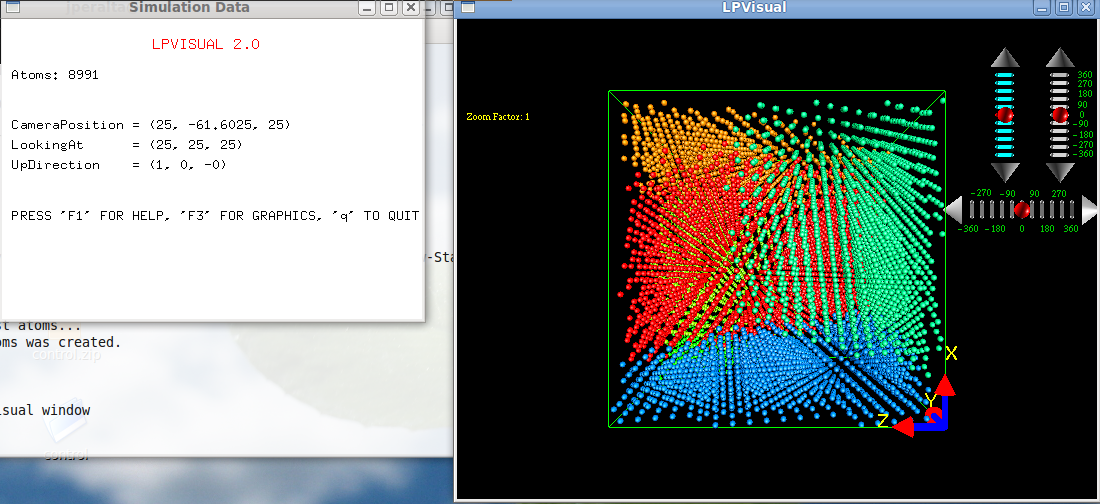
\includegraphics[scale=.35]{voronoi-1.png}
 \label{fig:voronoi-1}
 \caption{Screenshoot of \texttt{lpmd}. This use lpvisual to show the cell
generated using skewstart.}
\end{figure}

If you don't want to use or do not have installed lpvisual remove the option
\verb|-u lpvisual| from the command line and define some output to save this
configuration, for example \verb|-o xyz:file=output.xyz|. The results of the
quick-mode method are showed in the figure~\ref{fig:voronoi-1}. For the case
that you want to save this cell and visualize (using lpvisual), you will need
to execute in this way :

 \begin{verbatim}
 lpmd-visualizer -i voronoi:symbol=Fe,type=fcc,a=3.62,grains=6 \
 -u lpvisual -L 50,50,50 -o lpmd:file=new.lpmd,extra=rgb
\end{verbatim}

\subsection{skewstart}
This method was developed by \textit{K. Refson} for the molecular dynamics code
\textbf{moldy}. The goal of this method is build a atomic configuration
non-periodic and highly regular in order to guarantee a minimal space between
the atoms. The options availables in this plugin are :

\fb{
\begin{tabular}{lcl}
 symbol & = & Atomic symbol of the specie.\\
 atoms & = & Set the number of atoms inside of \\
 &&the cell.\\
\end{tabular}
}

As an example of how to use this plugin, consider a argon cell of 108 atoms in
a cell of size 20 \AA~. For this :

\begin{itemize}
 \item \textbf{Set the cristal details}
       \control{cell crystal a=20 b=20 c=20 alpha=90 beta=90 gamma=90}
 \item \textbf{Build the atoms positions using skewstart method}
       \control{input module=skewstart symbol=Ar}
\end{itemize}

Other examples can be found in
\url{http://www.lpmd.cl/Plugins/doku.php?id=plugins:cell_generators#crystal2d}.


%%%%%%%%%%%%%%%%%%%%%%%%%%%%%%%%%%%%%%%%%%%%%%%%%%%%%%%%%%%%%%%%%
%%%%%%%%%%%%%%%%%%%%%%%%%%%%%%%%%%%%%%%%%%%%%%%%%%%%%%%%%%%%%%%%%
\section{Cell managers plugins}

This plugins are responsable to generate the \textbf{smart lists} to realize
molecular dynamics simulation and/or analysis of atomic structures. This
\textbf{smart lists} help to reduce the calculation time during a process. The
scheme and extra information about this type of \textbf{cell-managers} could be
found in the work of Davis et al~\cite{Davis2010}.

\subsection{linkedcell}
This is the standard linkedcell list method, is one of the more fast and more
used method in Molecular dynamics. The improve for a large number of atoms is
huge in comparison with different types like minimumimage and is the most used
in defferent MD codes. This model generate subdivisions of the cell in the
different directions of the structure cell, is important keep in mind that the
subdivision size are minor that the minimum interaction distance between the
particles (related to the specific potential). However this, the plugin have an
auto-mode in order to make an automaic cell division.

\begin{itemize}
 \item \textbf{Loading the plugin}
       \control{use linkedcell \\ cutoff 2.0 \\ nx 10\\ ny 10\\ nz 10\\enduse}
 \item \textbf{Loading the plugin} \texttt{auto}.
       \control{use linkedcell \\ cutoff 2.0 \\ mode auto\\enduse}
 \item \textbf{Applying the plugin}
       \control{cellmanager linkedcell}
\end{itemize}

\subsection{minimumimage}
This plugin use the minimum-image model to realize the atomic interaction
process. Is frequently more slow, and only need the cutoff of the simulation as
a parameter. This method is useless when the cutoff is around the size of the
half of the simulation cell.

\begin{itemize}
 \item \textbf{Loading the plugin}
       \control{use minimumimage \\ cutoff 2.0 \\enduse}
 \item \textbf{Applying the plugin}
       \control{cellmanager minimumimage}
\end{itemize}

This will define our simulation using the minimumimage method with a
\verb|cutoff| of 2.0 \AA.

\subsection{lcbinary}
This plugin use the linkedcell method but in a different way that the explained
previously. This plugin modify the method and assign in an automatic way the
subdivision of the cell, allowing only one atom by cell. This method use a huge
quantity of RAM memory.

\begin{itemize}
 \item \textbf{Loading the plugin}
       \control{use lcbinary \\ cutoff 2.0 \\ mode auto\\enduse}
 \item \textbf{Applying the plugin}
       \control{cellmanager linkedcell}
\end{itemize}

If you have not clear what scheme of cellmanager use for your simulation, we
suggest to you to use the \verb|linkedcell| plugin in the \verb|auto| mode.

%%%%%%%%%%%%%%%%%%%%%%%%%%%%%%%%%%%%%%%%%%%%%%%%%%%%%%%%%%%%%%%%%
%%%%%%%%%%%%%%%%%%%%%%%%%%%%%%%%%%%%%%%%%%%%%%%%%%%%%%%%%%%%%%%%%
\section{Filter plugins}
This plugins are allowed to modify (in different ways) the simulation
structure. These can be used for the construction of new complex structures and
for apply specific properties to the structure. In a manner of example, these
plugins can be used to select a specific atomic region, and delete all the
others atoms that are not located in this region.

On the other hand, all the filter plugins can be applyied in a inverse way. So,
instead of keep the atoms in a specific region, you can delete the atoms of
that region using the flag :

\control{inverse=true}

\noindent
in the filter options. Other strong characteristic of the filter plugins, is
that these plugins can be applied using exceptions (\verb|except|) giving a
strong and more flexibility over the structure. More examples about the use of
these plugins can be found in the chapter~\ref{chap:exa} and in the website.

\subsection{box}
This plugin select the atoms locate in a rectangular region defined by the
plugin. The plugins options are :

\fb{
\begin{tabular}{lcl}
 x & = & Rango en la direcci\'on \texttt{x}.\\
 y & = & Rango en la direcci\'on \texttt{y}.\\
 z & = & Rango en la direcci\'on \texttt{z}.\\
\end{tabular}
}

Let's take a look in a single filter using the \verb|box| plugin.

\begin{itemize}
 \item \textbf{Delete all the atoms except these that are located in the region}
       \control{filter box x=0-5 y=0-6 z=10-15}

Using this, all the atoms of the simulation cell will disappear except the
atoms located in the $[0,5]$, $[0,6]$ and $[10,15]$ ranges of the $X$, $Y$ and
$Z$ axis. This is useful when we want to analyze a particular region of the
simulation cell.
 
 \item \textbf{Delete only the atoms located in the region.}
       \control{filter box x=0-5 y=0-6 z=10-15 inverse=true}

Using this, whe delete only the atoms in this particular regions, it means we
generate a rectangular hole in the simulation cell.
\end{itemize}

\subsection{element}
This plugin select the atomis by the atomic symbol. The options of the plugins
are :

\fb{
\begin{tabular}{lcl}
 symbol & = & Atomic symbol of the atoms to select.\\
\end{tabular}
}

Take an example of how to eliminate the Hydrogen atoms from a structure.

\begin{itemize}
 \item \textbf{Eliminate the} \texttt{H} \textbf{atoms}.
       \control{filter species symbol=H}
\end{itemize}


\subsection{index}
Select the atoms by their atomic index. This plugin is useful particularly for
old types of configurations where the atomic order in the file indicate some
specific characteristic. The options of this plugins are :

\fb{
\begin{tabular}{lcl}
 index & = & List with the atomic index.\\
\end{tabular}
}

For example elminiate the atoms from the 1 to 3 and then from the 1 to the 50.

\begin{itemize}
 \item \textbf{Deleting atoms from 1 to 3}.
       \control{filter index index=1,2,3}
 \item \textbf{Deleting atoms from 1 to 50}.
       \control{filter index index=1-50}
\end{itemize}

\subsection{sphere}
Select the atoms in a spherical region. the option of this plugins are :

\fb{
\begin{tabular}{lcl}
 radius & = & Sphere radius in \AA.\\
 center & = & Sphere center, write like vector $\langle a,b,c\rangle$.\\
\end{tabular}
}

For example select the atoms only in a spherical region of a structure of
100\AA by side, locating the sphere in the center of the simulation box, with a
radius of 10\AA.

\begin{itemize}
 \item \textbf{Spherical selection}.
       \control{filter sphere radius=10 center=<50,50,50> inverse=true}
\end{itemize}

\subsection{tag}
This plugin allow select the atoms that have some specific tag. In {\lpmd} you
can assign specific tag to the atoms (practically any word is allowed), however
there are some specific keyword reserved too bye {\lpmd}, like \verb|fixedpos|,
\verb|fixedvel| and \verb|fixedacc| that are controlled by the \texttt{API}.
The option of the tag plugins are :

\fb{
\begin{tabular}{lcl}
 name & = & Tag name.\\
 value & = & Boolean true or flase, on the tag condition.\\
\end{tabular}
}

Select for example the atoms that have fixed position and remove it from the
structure.

\begin{itemize}
 \item \textbf{Select the atoms with fixed position, and delete it}.
       \control{filter tag name=fixedpos value=true}
\end{itemize}

%%%%%%%%%%%%%%%%%%%%%%%%%%%%%%%%%%%%%%%%%%%%%%%%%%%%%%%%%%%%%%%%%
%%%%%%%%%%%%%%%%%%%%%%%%%%%%%%%%%%%%%%%%%%%%%%%%%%%%%%%%%%%%%%%%%
\section{Modifiers plugins}
This type of plugins can modify specific characteristics of a atomic set or the
full simulation cell. That mean that this modifiers plugin can be applied in a
filtered way, for example :

\control{apply modify-plugin start=... end=... each=... over\textbackslash
filter-module <filter-options>}

This allow us more flexibility in the control of the simulation. On the other
hand if we want to modify the full simulaiton cell, we can use : 

\control{apply modify-module start=... end=... each=...}

Some plugins, like cellscaling can be applied only in the complete
simulation cell.

\subsection{berendsen}
This plugin control and scale the temperature. The scaling methodology used by
the plugin is widely used because is not a hard scaling process like the
\verb|tempscaling| plugin method, allowing a more effective thermalization
process of the structre. 

The equation that describe the Berendsen thermostat is :

$$\frac{dT}{dt} = \frac{T_0 - T}{\tau}$$

\noindent
where $\frac{dT}{dt}$ is  the temperature variation ...

The options allowed in this plugin are :

\fb{
\begin{tabular}{lcl}
 from & = & Initial temperature.\\
 to & = & Final temperature.\\
 tau & = & Termostat interval.\\
\end{tabular}
}

\subsection{cellscaling}
This plugin can change the size of the simulation cell (remember that the
modifier modules can be applied during the simulation or over a single atomic
structure). This plugin is useful to sudy the behaviour of materials under
different densities, in one sinlge simulation process. The options of the
plugins are :

\fb{
\begin{tabular}{lcl}
 percent & = & Indicate the percent that the cell axis will change \\
 axis & = & Indicate the axis to compress (x,y,z, or all). \\
 constant & = & true/false Indicate if the change is constant respect\\
 && to the initial value.\\
\end{tabular}
}

With this plugin we can do hydrostatic or unidirectional compression or
expansion of the cell lenghts. And control the scaling factor constant or not.

\subsection{displace}
This plugin modify the atomic position of the system, using a vectorial
displacement of the atoms. The options of this plugins are :

\fb{
\begin{tabular}{lcl}
 x & = & Displace in x axis in \AA.\\
 y & = & Displace in y axis in \AA.\\
 z & = & Displace in z axis in \AA\\
\end{tabular}
}

\subsection{moleculecm}
Generate diatomics molecules. Foer each atoms in the structure, this plugin
looks for closer atoms (in a specific radius). If the distance between the
atoms is minor or equal the atoms are considered bonded. If the atoms are
bonded both atoms are deleted and replaced by a new atoms located in the center
of mass of both atoms.

\fb{
\begin{tabular}{lcl}
 radius & = & Cutoff radius around each atom.\\
\end{tabular}
}


\subsection{propertycolor}
This plugin assignate colors to the atoms, by some specific condition. The
principal option of the plugins are :

\fb{
\begin{tabular}{lcl}
 property & = & Property to color.(temperature, velocity, acceleration,
neighbours)\\
 min & = & Minimum value of the property.\\
 max & = & Maximum value of the property.\\
 cutoff & = & Some properties need cutoff.\\
 filterby & = & Filter by.\\
\end{tabular}
}

Like an example let's color the atoms by their temperature, and associate 300K
to the minimum temperature and 500K to the maximum temperature. So to assign
colors to the atoms we will use :

\begin{itemize}
 \item \textbf{Load the plugin}
       \control{use propertycolor as temp\\ min 300\\ max 300\\enduse}
 \item \textbf{Applying the plugin}
       \control{apply temp start=1 end=1000 each=2}
\end{itemize}

\subsection{quenchedmd}
This plugin use the \textit{Quenched Molecular Dynamics} method to find the
structure of minimum energy. During the processs the integrator do not
have a molecular dynamics behaviour, this only is used to verify the
projection between the force and the velocity, value that is forced if
the energy increase. 

\fb{
\begin{tabular}{lcl}
 debug & = & Show information debug.\\
\end{tabular}
}

This plugins do not require special options, is only loaded and applied. Note
that the \verb|debug| is an option for almos all the plugins.

\subsection{randomatom}
This plugin is used to eliminate or modify atoms of a structure in a random
way. The principal options of the plugins are :

\fb{
\begin{tabular}{lcl}
 type & = & Action delete/replace.\\
 value & = & Porcentual value of the number of atoms to replace.\\
 symbol & = & Atomic symbol for the case of replace.\\
 density & = & fixed/free the density of the sample.\\
\end{tabular}
}

Like an example, remove random atoms from a crystal to generate vacancies.

\begin{itemize}
 \item \textbf{Loading plugin}
       \control{use randomatom\\ type delete\\ value 5\\ density fixed\\enduse}
 \item \textbf{Applying the plugin.}
       \control{apply randomatom}
\end{itemize}

Remember that you can apply the plugins in a specific step of time using
\texttt{start=10 end=10 each=1} options.

\subsection{replicate}
This plugin replicate the simulation cell in their different axis. The options
of the plugins are :

\fb{
\begin{tabular}{lcl}
 nx & = & Number of repetitions in \texttt{x}.\\
 ny & = & Number of repetitions in \texttt{y}.\\
 nz & = & Number of repetitions in \texttt{z}.\\
\end{tabular}
}
The repetitions mus tbe integers numbers, usually this plugin is only used in
the beginin of the simulation and can be called with the \verb|prepare| option
of the control file. Is important highlight that when we modify the structure
changing the number of atoms, the \verb|optimize-simulation| flag must be
deactivated :

\begin{itemize}
 \item \textbf{Deactivate the initial optimization}
       \control{set optimize-simulation false}
\end{itemize}


\subsection{rotate}
This plugin modify the atoms positions, rotating the atoms in a specific degree
around a origin. The options of the plugins are :

\fb{
\begin{tabular}{lcl}
 x & = & x coordinate of rotation origin.\\
 y & = & y coordinate of rotation origin.\\
 z & = & z coordinate of rotation origin.\\
 angle & = & Rotation angle in degrees.\\
\end{tabular}
}

\subsection{setcolor}
This plugin can assign color to the atoms. The color is assigned in RGB format
with values betwee 0 and 1. The option are :

\fb{
\begin{tabular}{lcl}
 color & = & Color of the atom in a vector format.\\
\end{tabular}
}

Like an example set the atoms color to red for all the atoms.

\begin{itemize}
 \item \textbf{Loading the plugin}
       \control{use setcolor as red\\ color <1.0,0.0,0.0>\\enduse}
 \item \textbf{Applying the plugin}
       \control{apply setcolor}
\end{itemize}

\subsection{settag}
This plugin is used to assign a tag to a atom group, and the current status of
the tag with a boolean value. The options of the plugins are :

\fb{
\begin{tabular}{lcl}
 name & = & Tag name\\
 value & = & Tag status true/false\\
\end{tabular}
}

Like an example assign fixed position to a set of atoms in the structure, i.e.
the atoms will not move during the simulation. Remember that \verb|fixedpos| is
a specific reserved tag used in {\lpmd}.

\begin{itemize}
 \item \textbf{Loading plugin}
       \control{use settag as pos\\ name fixedpos\\ value true\\enduse}
 \item \textbf{Applying plugin}
       \control{apply pos}
\end{itemize}

Usually modifiers like \verb|settag| or \verb|setcolor| are used with filters,
so is enough if we specify the filter in the \verb|aaply| line.

\subsection{setvelocity}
This plugin is used to assign velocities to a group of atoms. the options of
the plugins are :

\fb{
\begin{tabular}{lcl}
 velocity & = & Velocity to assing in a vector format.\\
\end{tabular}
}

\subsection{shear}
This plugin is used to make a shear on the structure, modifying the cell
vectors. The principal arguments of this plugins are :

\fb{
\begin{tabular}{lcl}
 axis & = & Axis where the shear will be made.\\
 normal & = & Perpendicular axis to the shear.\\
 strain & = & Maximum displacement to apply strain*L(normal)\\
\end{tabular}
}

With this we can apply shear to the simulation. Like an example, let's apply
shear over the original cell, so we will use :

\control{prepare shear axis=X normal=Y strain=0.01}

\subsection{temperature}
This plugin apply temperature to a group of atoms. The options of the plugins
are :

\fb{
\begin{tabular}{lcl}
 t & = & Temperature to set to a atoms group.\\
\end{tabular}
}

Youc an use this module too to set the initial temperature of the simulation.

\control{prepare temperature t=300}

\subsection{tempscaling}
This plugin is used to control the temperature in the structure. This plugin
use velocity rescaling procedure, that is one of the more used methods in MD. 

The scaling procidure modify the atoms velocity of the atoms using the factor :

$$s=\sqrt{\frac{gk_BT}{2\mathcal{K}}}$$

Remember that the process of control of temperature do not give real
thermodinamcial averages. For this reason is necessary realize the averages
after the rescaling process. The option of the plugins are :

\fb{
\begin{tabular}{lcl}
 from & = & Initial temperature.\\
 to & = & Final temperature.\\
\end{tabular}
}

Let use a big example where a Ar sample is heated to 300K, then the
temperetature is controlled for a while, and finally the system is free and
running.

First we will load the plugins for each step.

\begin{itemize}
 \item \textbf{Loading for heating}
       \control{use cellscaling as uptemp \\   from 84.0\\   to 300.0\\enduse}
 \item \textbf{Loading for control}
       \control{use cellscaling as fixtemp \\   from 300.0\\   to 300.0\\enduse}
\end{itemize}

Now we apply this modules during different steps of the simulations.

\begin{itemize}
 \item \textbf{Applying \textbf{uptemp} fro 1 to 10000, each 50 steps.}
       \control{apply uptemp start=1 end=10000 each=50}
 \item \textbf{Control temperature between 10000 and 15000.}
       \control{apply fixtemp start=10000 end=15000 each=50}
\end{itemize}

After the step 15000 the simulation will not use anymore the temperature
scaling procedure.

\subsection{undopbc}
This plugin is used to undo the perioduc boundeary condition of a structure, is
used principally for undo this from MD configurations set.

This plugin do not use any special option, only loaded and applyed. Like an
example remove let's remove the periodicity of a configuration cell.

\begin{itemize}
 \item \textbf{Loading the plugin}
       \control{use undopbc \\enduse}
 \item \textbf{Applying the plugin}
       \control{apply undopbc start=.. end=.. each=..}
\end{itemize}


%%%%%%%%%%%%%%%%%%%%%%%%%%%%%%%%%%%%%%%%%%%%%%%%%%%%%%%%%%%%%%%%%
%%%%%%%%%%%%%%%%%%%%%%%%%%%%%%%%%%%%%%%%%%%%%%%%%%%%%%%%%%%%%%%%%
\section{Instantaneous properties plugins}
Las propiedades instant\'aneas son aquellas que se pueden evaluar en cualquier
instante de tiempo sobre una configuraci\'on at\'omica, las que se listan a
continuaci\'on son las que se han implementado a la fecha en {\lpmd}.

Estas propiedades adem\'as de ser analizadas \textit{post-simulaci\'on} pueden
lelvarse acabo durante la simulaci\'on misma.

\subsection{angdist}
Calcula la distribucion angular de la celda de simulaci\'on. Para determinar los
\'angulos caracter\'isticos de una celda de simulaci\'on es necesario entender
el esquema o preocedimiento:
\begin{enumerate}
 \item Se selecciona un \'atomo $i$.
 \item Se busca un \'atomo $j$ que se encuentre dentro del radio de corte $r_{ij}$
 \item Se busca un \'atomo $k$ que se enceuntre dentro del radio de corte $r_{ik}$
 \item Se calcula el \'angulo  $\angle j-i-k$ y se a\~nade en la cuenta
\end{enumerate}

De esta forma obtenemos una funci\'on entre 0 y 180$^\circ$ que nos muestra
cuales son los principales angulos de ``enlace'' o ``distancia'' de los
\'atomos. Las opciones de uso son:

\fb{
\begin{tabular}{lcl}
 bins & = & N\'umero de intervalos entre 0 y 180 grados. \\
 atoms & = & N\'umero de especies at\'omicas y los s\'imbolos\\
&&asociados a cada una.\\
 rcut & = & Se especifican 2 especies at\'omicas y su radio\\
&&de corte.\\
 output & = & Archivo de salida.\\
 average & = & Se promediar\'an o no los calculos.\\
\end{tabular}
}

\subsection{atomtrail}
Calcula la ... en 2 y 3 dimensiones.
\begin{enumerate}
 \item Se ..
 \item Se ..
\end{enumerate}

De esta forma obtenemos una funci\'on entre 0 y 180$^\circ$ que nos muestra
cuales son los principales angulos de ``enlace'' o ``distancia'' de los
\'atomos. Las opciones de uso son:

\fb{
\begin{tabular}{lcl}
 nx & = & N\'umero de intervalos en \texttt{x}. \\
 ny & = & N\'umero de intervalos en \texttt{y}. \\
 nz & = & N\'umero de intervalos en \texttt{z}. \\
 plane & = & Plano XY,YZ, etc.\\
 mode & = & 2D o 3D.\\
\end{tabular}
}

\subsection{cna}
Calcula el n\'umero de cordinaci\'on de la celda, informandonos a modo de
histograma, como se han encontrado los n\'umeros de vecinos asociados a la
muestra. La manera de calcular este numero de coordinacion es:

\begin{enumerate}
 \item Se genera un arreglo entre 0 y el m\'aximo n\'umero de vecinos posibles.
 \item Para cada \'atomo $i$, se ve cuantos vecinos $j$ tiene dentro de un radio
d corte $r_{ij}$.
 \item Se entrega un valor porcentual del conteo previo.
\end{enumerate}

\fb{
\begin{tabular}{lcl}
 maxn & = & N\'umero m\'aximo d vecinos para el histograma.\\
 atoms & = & N\'umero de especies at\'omicas y los s\'imbolos\\
&&asociados a cada una.\\
 rcut & = & Se especifican 2 especies at\'omicas y su radio\\
&&de corte.\\
 output & = & Archivo de salida.\\
 average & = & Se promediar\'an o no los calculos.\\
\end{tabular}
}

\subsection{cordnumfunc}
Calcula el n\'umero de cordinaci\'on de la celda, en este caso es la funci\'on
m\'as usada n publicaciones, pero en ocaciones puede ser m\'as simple de
analizar, el m\'etodo \textbf{cordnum}. Corresponde tambi\'en a la integraci\'on
de la funci\'on de distribuci\'on de pares.
\begin{enumerate}
 \item Se selecciona una distancia m\'axima y se divide en intervalos.
 \item Se selecciona un \'atomo $i$.
 \item Se analiza cuantos atomos $j$ caen en la distancia asociada al intervalo.
 \item Se continua de forma acumulativa, hasta un valor rasonable.
\end{enumerate}

La forma de utilizar el m\'etodo esta dada por:

\fb{
\begin{tabular}{lcl}
 bins & = & N\'umero m\'aximo de intervalos entre 0 y \textbf{rcut}.\\
 atoms & = & N\'umero de especies at\'omicas y los s\'imbolos\\
&&asociados a cada una.\\
 rcut & = & Radio de corte m\'aximo para an\'alisis.\\
 output & = & Archivo de salida.\\
 average & = & Se promediar\'an o no los calculos.\\
\end{tabular}
}

\subsection{cordnum}
Calcula el n\'umero de cordinaci\'on de la celda, en este caso es la funci\'on
m\'as usada n publicaciones, pero en ocaciones puede ser m\'as simple de
analizar, el m\'etodo \textbf{cordnum}. Corresponde tambi\'en a la integraci\'on
de la funci\'on de distribuci\'on de pares.
\begin{enumerate}
 \item Se selecciona una distancia m\'axima y se divide en intervalos.
 \item Se selecciona un \'atomo $i$.
 \item Se analiza cuantos atomos $j$ caen en la distancia asociada al intervalo.
 \item Se continua de forma acumulativa, hasta un valor rasonable.
\end{enumerate}

La forma de utilizar el m\'etodo esta dada por:

\fb{
\begin{tabular}{lcl}
 bins & = & N\'umero m\'aximo de intervalos entre 0 y \textbf{rcut}.\\
 atoms & = & N\'umero de especies at\'omicas y los s\'imbolos\\
&&asociados a cada una.\\
 rcut & = & Radio de corte m\'aximo para an\'alisis.\\
 output & = & Archivo de salida.\\
 average & = & Se promediar\'an o no los calculos.\\
\end{tabular}
}

\subsection{densityprofile}
Calc\'ula un perfil de densidades bidimensional. Este m\'etodo divide la celda
de simulaci\'on en cajas pequenas, en una direccion privilegiada y calcula las
densidades en cada una de ellas, da una idea muy clara de la densidad ``por
secci\'on'' de la celda de simulaci\'on.

La forma de utilizarla es:

\fb{
\begin{tabular}{lcl}
 axis & = & Valor del eje preferencial, o direcci\'on, del c\'alculo.\\
 bins & = & N\'umero de intervalos para dividir el eje.\\
 range & = & Rango espacial de cada uno de los ejes, con \\
 && formato: nombre del eje, m\'inimo y m\'aximo.\\
 output & = & Archivo de salida.\\
 average & = & Se promediar\'an o no los calculos.\\
\end{tabular}
}


\subsection{gdr}
Caulcula la funcion de distribucion de pares de la celda. Es uno de los
m\'etodos utilizados para determinar las distancias principales a primeros y
segundos vecinos de una celda de simulaci\'on. El procedimiento es el siguiente:
\begin{enumerate}
 \item Se selecciona un \'atomo $i$.
 \item Se ve cuantos atomos $j$ estan dentro de un cascar\'on esf\'erico
centrado en $i$.
 \item Se promedia sobre los \'atomos asociados.
\end{enumerate}

\fb{
\begin{tabular}{lcl}
 bins & = & N\'umero m\'aximo de intervalos entre 0 y \textbf{rcut}.\\
 rcut & = & Radio de corte m\'aximo para an\'alisis.\\
 output & = & Archivo de salida.\\
 average & = & Se promediar\'an o no los calculos.\\
\end{tabular}
}

\subsection{localpressure}

Calcula una presion local de la celda de simulaci\'on, para eso utiliza el
stress de los \'atomo en cada ``sub-celda'', los valores entregados,
recomendamos graficarlos con escala de colores para poder observar fen\'omenos. 

La forma de utilizar el plugin es:
\fb{
\begin{tabular}{lcl}
 rcut & = & Radio de corte.\\
 n$\alpha$ & = & Divisiones para cada eje ($\alpha=x,y,z$).\\
 output & = & Archivo de salida.\\
 average & = & Se promediar\'an o no los calculos.\\
\end{tabular}
}

\subsection{overlap}

Calcula una presion local de la celda de simulaci\'on, para eso utiliza el
stress de los \'atomo en cada ``sub-celda'', los valores entregados,
recomendamos graficarlos con escala de colores para poder observar fen\'omenos. 

La forma de utilizar el plugin es:
\fb{
\begin{tabular}{lcl}
 rcut & = & Radio de corte.\\
 n$\alpha$ & = & Divisiones para cada eje ($\alpha=x,y,z$).\\
 output & = & Archivo de salida.\\
 average & = & Se promediar\'an o no los calculos.\\
\end{tabular}
}

\subsection{pairdistances}

Calcula una presion local de la celda de simulaci\'on, para eso utiliza el
stress de los \'atomo en cada ``sub-celda'', los valores entregados,
recomendamos graficarlos con escala de colores para poder observar fen\'omenos. 

La forma de utilizar el plugin es:
\fb{
\begin{tabular}{lcl}
 rcut & = & Radio de corte.\\
 n$\alpha$ & = & Divisiones para cada eje ($\alpha=x,y,z$).\\
 output & = & Archivo de salida.\\
 average & = & Se promediar\'an o no los calculos.\\
\end{tabular}
}

\subsection{rvcorr}

Calcula una presion local de la celda de simulaci\'on, para eso utiliza el
stress de los \'atomo en cada ``sub-celda'', los valores entregados,
recomendamos graficarlos con escala de colores para poder observar fen\'omenos. 

La forma de utilizar el plugin es:
\fb{
\begin{tabular}{lcl}
 rcut & = & Radio de corte.\\
 n$\alpha$ & = & Divisiones para cada eje ($\alpha=x,y,z$).\\
 output & = & Archivo de salida.\\
 average & = & Se promediar\'an o no los calculos.\\
\end{tabular}
}

\subsection{sitecoord}

Calcula una presion local de la celda de simulaci\'on, para eso utiliza el
stress de los \'atomo en cada ``sub-celda'', los valores entregados,
recomendamos graficarlos con escala de colores para poder observar fen\'omenos. 

La forma de utilizar el plugin es:
\fb{
\begin{tabular}{lcl}
 rcut & = & Radio de corte.\\
 n$\alpha$ & = & Divisiones para cada eje ($\alpha=x,y,z$).\\
 output & = & Archivo de salida.\\
 average & = & Se promediar\'an o no los calculos.\\
\end{tabular}
}


\subsection{tempprofile}
Calc\'ula un perfil de temperaturas bidimensional. Al igual que el m\'etodo
anterior, se divide la caja en celdas pequenas, en donde calculamos la
temperatura de cada una de ellas.

La forma de utilizar esto es:

\fb{
\begin{tabular}{lcl}
 axis & = & Valor del eje preferencial, o direcci\'on, del c\'alculo.\\
 bins & = & N\'umero de intervalos para dividir el eje.\\
 range & = & Rango espacial de cada uno de los ejes, con formato:\\
&&nombre del eje, m\'inimo y m\'aximo.\\
 output & = & Archivo de salida.\\
 average & = & Se promediar\'an o no los calculos.\\
\end{tabular}
}

\subsection{veldist}
Muestra como estan distribuidas las velocidades del sistema. La salida es un
histograma de velocidades. La forma de uso es:

\fb{
\begin{tabular}{lcl}
 bins & = & N\'umero de intervalos para dividir el histograma.\\
 output & = & Archivo de salida.\\
 average & = & Se promediar\'an o no los calculos.\\
\end{tabular}
}

%%%%%%%%%%%%%%%%%%%%%%%%%%%%%%%%%%%%%%%%%%%%%%%%%%%%%%%%%%%%%%%%%
%%%%%%%%%%%%%%%%%%%%%%%%%%%%%%%%%%%%%%%%%%%%%%%%%%%%%%%%%%%%%%%%%
\section{Dynamical properties plugins}
Las porpiedades din\'amicas, \textbf{no} pueden ser calculadas durante la
simulaci\'ond e din\'amica molecular, ya que poseen correlaci\'on temporal en su
an\'alisis, es por ello que estos m\'odulos no deben ser cargados en un fichero
de control para {\lpmd}. Sin embargo estas propiedades pueden calcularase a
partir de los ficheros de salida, tales como \verb|xyz| o \verb|lpmd|,
utilizando \verb|lpmd-analyzer|.
\subsection{dispvol}
Calcula el desplazamiento cuadratico medio del sistema. Por el momento el plugin
esta en etapa de mejora y documentaci\'on.
\subsection{mobility}
Calcula el desplazamiento cuadratico medio del sistema. Por el momento el plugin
esta en etapa de mejora y documentaci\'on.
\subsection{msd}
Calcula el desplazamiento cuadratico medio del sistema. Por el momento el plugin
esta en etapa de mejora y documentaci\'on.
\subsection{vacf}
Calcula la funci\'on de autocorrelaci\'on de velocidades de la celda. Por el
momento el plugin esta en etapa de mejora y documentaci\'on.


%%%%%%%%%%%%%%%%%%%%%%%%%%%%%%%%%%%%%%%%%%%%%%%%%%%%%%%%%%%%%%%%%
%%%%%%%%%%%%%%%%%%%%%%%%%%%%%%%%%%%%%%%%%%%%%%%%%%%%%%%%%%%%%%%%%
\section{Integrators plugins}
\subsection{beeman}
El algoritmo de Beeman es un m\'etodo para integrar num\'ericamente ecuaciones
difereciales, para el caso de din\'amica molecular, la posici\'on y velocidad,es
similar al m\'etodo de verlet, pero las velocidades son con mejor precisi\'on.

Las f\'ormulas para posici\'on y velocidad estan dadas por:

$$r(t+\Delta t) = r(t) + v(t)\Delta t + \frac{2}{3}a(t)\Delta t^2 -
\frac{1}{6}a(t-\Delta t)\Delta t^2 +\mathcal{O}(\Delta t^4)$$
$$v(t+\Delta t) = v(t) + \frac{1}{3}a(t+\Delta t)\Delta t+\frac{5}{6}a(t)\Delta
t-\frac{1}{6}a(t-\Delta t)\Delta t+\mathcal{O}(\Delta t^3)$$

\subsection{euler}
El integrador de Euler, es el m\'atodo n\'umerico de primer orden para resolver
ecuaciones diferenciales ordinarias. Este es el m\'etodo m\'as b\'asico para la
integraci\'on num\'erica de las ecuaciones.

Las f\'ormulas para posici\'on esta dada por:

$$r(t+\Delta t) = r(t) + h\times f(t,r(t))$$

\subsection{hardspheres}
Es un m\'etodo de integraci\'on que calcula las posiciones y velocidades de
forma alternada. Las posiciones y velocidades estan dadas por:

\subsection{leapfrog}
Es un m\'etodo de integraci\'on que calcula las posiciones y velocidades de
forma alternada. Las posiciones y velocidades estan dadas por:
$$r(t+\Delta t) = r(t) + v(t)\Delta t + a(t)\frac{\Delta t^2}{2}$$
$$v(t+\Delta t) = v(t) + \frac{a(t)+a(t+\Delta t)}{2}\Delta t$$

\subsection{metropolis}
Es un m\'etodo de integraci\'on que calcula las posiciones y velocidades de
forma alternada. Las posiciones y velocidades estan dadas por:

\subsection{nosehoover}
Es utilizado para simulacion de ensambles de tipo NVT, en general el m\'etodo
corresponde a una modificaci\'on de las ecuaciones de movimiento, donde aparece
una masa ficticia en las ecuaciones a resolver.

% \subsection{nullintegrator}
% Integrador nulo, solo en caso de que no se requiera mover el sistema, es decir
% las particulas simplemente \textit{congeladas}.

\subsection{velocityverlet}
M\'etodo similar al de verlet, pero con mejoras respecto a la performance en la
integraci\'on, incorporando directamente la velocidad en el sistema, las
ecuaciones estan dadas por:
$$r(t+\Delta t) = r(t) - v(t)\Delta t + \frac{1}{2}a(t)\Delta t^2$$
$$v(t+\Delta t) = v(t) + \frac{a(t) - a(t + \Delta t)}{2}\Delta t$$

\subsection{verlet}
Es un m\'etodo utilizado para integrar las ecuaciones de Newton de movimiento,
las posiciones y velocidades del sistema estan dadas por:
$$r(t+\Delta t) = 2r(t) - r(t-\Delta t) + a(t)\Delta t^2 + \mathcal{O}(\Delta t^4)$$
$$v(t+\Delta t) = \frac{r(t+\Delta t) - r(t)}{\Delta t} + \mathcal{O}(\Delta t)$$



%%%%%%%%%%%%%%%%%%%%%%%%%%%%%%%%%%%%%%%%%%%%%%%%%%%%%%%%%%%%%%%%%
%%%%%%%%%%%%%%%%%%%%%%%%%%%%%%%%%%%%%%%%%%%%%%%%%%%%%%%%%%%%%%%%%
\section{Pair interatomic potential plugins}
\subsection{buckingham}
\fb{\begin{minipage}{10cm}Buckingham, no incluye directamente parte coulombiana,
para ello es necesario a\~nadir como un potencial adicional a ewald u otro
similar que a\~nada la parte coulombiana.\end{minipage}}

Est\'e m\'odulo especif\'ica la interacci\'on de buckingham entre los \'atomos,
de esta forma, la energ\'ia producida por la interacci\'on de dos part\'iculas
$i$ y $j$, queda

$$E(\vec{r}_{ij}) = B1 \exp\left(-\frac{|\vec{r}_{ij}|}{\rho}\right) -
\frac{B2}{(|\vec{r}_{ij}|)^6}$$

y la fuerza,

$$\vec{F}(\vec{r}_{ij}) =
-\frac{B1\exp\left(-\frac{|\vec{r}_{ij}|}{\rho}\right)}{|\vec{r}_{ij}|\rho}\vec{
r}_{ij} + \frac{6B2}{|\vec{r}_{ij}|^8}\vec{r}_{ij}$$

Las palabras reservadas por el plugin \textbf{buckingham}, son :

\fb{
\begin{tabular}{lcl}
 B1 & = & indica el valor de la constante B1.\\
 B2 & = & indica el valor de la constante B2.\\
 Ro & = & el valor de rho para el potencial.\\
 cutoff & = & indica el cutoff del potencial.\\
\end{tabular}
}

\subsection{constantforce}
Aplica una fuerza constante sobre cada \'atomo. Si $m$ es la masa del \'atomo,
la aceleraci\'on del \'atomo provocada por el potencial interat\'omico tendr\'a
un t\'ermino adicional $\vec F/m$. Todos los \'atomos seleccionados ser\'an
afectados por la misma fuerza, pero no acelerar\'an igual si poseen distinta
masa.

Se utiliza principalmente para aplicarles fuerzas a especies at\'omicas o bien a
atomos seleccionados de alguna forma en especial. Este \textit{potencial}, no
retorna una energ\'ia (cero) y s\'olo tiene capacidad de asignar una fuerza
constante a un set de atomos.\\
                                       
Cargando el M\'odulo :
\control{
  use constantforce as gravity\\
  force <0.0,0.0,-4.06E-16>\\
   enduse\\
}

Llamando al m\'odulo :

  \control{potential gravity Ar Ar}

En este ejemplo agregamos la aceleraci\'on de gravedad $g=-9.8\left[m\over
s^2\right]$ a los \'atomos de arg\'on, de masa $m=39.948 [amu]$, para lo cual se
necesita una fuerza de $F=m*a=-391.4904 \left[amu*m\over
s^2\right]=-4.06\times10^{-16}\left[eV\over \text\AA\right]$ (el usuario es
responsable de discernir si los ordenes de magnitud son razonables).\\

La fuerza debe ser ingresada en unidades de $\left[eV \over \text\AA\right]$
($E=F\cdot d\ \Rightarrow F=E/d$), la cual es convertida internamente por
{\lpmd} a las unidades naturales del programa, $\left[amu*\text\AA\over
fs^2\right]$. Esto permite dividir la fuerza ingresada por la masa del elemento
(en este caso, arg\'on), la cual est\'a en unidades de masa at\'omica ($amu$),
quedando un factor con unidades de aceleraci\'on medida en $\left[\text\AA\over
fs^2\right]$, la cual es adicionada a la aceleraci\'on producida por el
potencial interat\'omico.


Las palabras reservadas por el plugin \textbf{constantforce}, son :

\fb{
\begin{tabular}{lcl}
 forcevector & = & indica de la fuerza constante a aplicarse.\\
\end{tabular}
}

\subsection{harmonic}
Potencial arm\'onico entre especies at\'omicas. De manera similar a un potencial
de morse, tenemos que la energ\'ia que sienten las part\'iculas $i$ y $j$ a
causa de la interacci\'on a trav\'es de \'este potencial es,

$$E(\vec{r}_{ij}) = \frac{1}{2}k\left(|\vec{r}_{ij}|-a\right)^2$$

En donde $k$ es la constante de elasticidad y $a$ la separaci\'on de equilibrio.
Con esto la fuerza para el potencial arm\'onico esta dada por,

$$\vec{F}(\vec{r}_{ij}) = \frac{k}{|\vec{r}_{ij}|}\left(|\vec{r}_{ij}|-a\right)$$

Las palabras reservadas por el plugin \textbf{harmonic}, son :

\fb{
\begin{tabular}{lcl}
 k & = & indica el valor de la constante de elasticidad.\\
 a & = & indica el valor de el largo de equilibrio.\\
 cutoff & = & indica el cutoff del potencial.\\
\end{tabular}
}

\subsection{lennardjones}
El m\'odulo \textbf{lennardjones} hace referencia al potencial de Lennard-Jones,
que es de la forma,
$$U(r_{ij}) =
4\epsilon\left(\left(\frac{\sigma}{r_{ij}}\right)^{12}-\left(\frac{\sigma}{r_{ij
}}\right)^6\right)$$

En donde $r_{ij}$ es la distancia interat\'omica de los \'atomos $i$ y $j$. 

Para el c\'alculo de Fuerzas, la forma del potencial que nos interesa, es
aquella fuerza que siente el \'atomo $i$ producida por el \'atomo $j$, la que
debe ser implementada en el plugin, para potentiales de pares, para el caso del
potencial de Lennard Jones, la fuerza esta dada por,

$$F_{ij} = \frac{-48.0\epsilon}{r_{ij}^2}\left(
\left(\frac{\sigma}{r_{ij}}\right)^{12} +
\frac{1}{2}\left(\frac{\sigma}{r_{ij}}\right)^6 \right) \vec{r_{ij}}$$

en donde $\vec{r_{ij}}$ es el vector distancia entre los \'atomos $i$ y $j$, y
$r_{ij}$ es la distancia entre ellos. 

Las palabras reservadas por el plugin \textbf{lennardjones}, son :

\fb{
\begin{tabular}{lcl}
 epsilon & = & indica el valor de epsilon.\\
 sigma & = & indica el valor de sigma.\\
 cutoff & = & indica el cutoff del potencial.\\
\end{tabular}
}

Las unidades en que deben ser ingresados, las constantes, deben ser basadas en
que las distancias estan en [\AA] y la energ\'ia debe ser adquirida en [eV].

\subsection{morse}
Utiliza Potencial de Morse para la interacci\'on de las especies at\'omicas. La
energ\'ia que siente una part\'icula $i$ a causa de la precensia de otra
part\'icula $j$, si ambas interactuan con un potencial de este estilo, esta dada
por :

$$E(\vec{r}_{ij}) = D_e\left(1-\exp(-a(\vec{r}_{ij}-\vec{r}_e))\right)^2$$

en donde $D_e$ es la profundidad del pozo, $a$ es el ancho del pozi y $r_e$ es
la distancia en equilibrio. Y entonces, la fuerza que siente un \'atomo $i$
producto de otro \'atomo $j$ est\'a dada por,

$$\vec{F}_{ij} ( \vec{r}_{ij}) =
2aD_e\exp(-a(\vec{r}_{ij}-\vec{r}_e))\left(1-\exp(-a(\vec{r}_{ij}-\vec{r}
_e))\right)\frac{\vec{r}}{|\vec{r}|}$$

Las palabras reservadas por el plugin \textbf{morse}, son :

\fb{
\begin{tabular}{lcl}
 depth & = & indica el valor de profundidad del pozo.\\
 a & = & indica el valor del ancho del pozo.\\
 re & = & indica el largo de enlaze en equilibrio.\\
 cutoff & = & indica el cutoff del potencial.\\
\end{tabular}
}

% \subsection{nullpairpotential}
% Utiliza Potencial de LJ tabulado. De forma similar al m\'odulo anterior pero
% porcentualmente m\'as r\'apido. Es recomendable utilizarlo para sistemas con grn
% n\'umero de part\'iculas.

\subsection{tabulatedpair}
Utiliza Potencial de LJ tabulado. De forma similar al m\'odulo anterior pero
porcentualmente m\'as r\'apido. Es recomendable utilizarlo para sistemas con grn
n\'umero de part\'iculas.


%%%%%%%%%%%%%%%%%%%%%%%%%%%%%%%%%%%%%%%%%%%%%%%%%%%%%%%%%%%%%%%%%
%%%%%%%%%%%%%%%%%%%%%%%%%%%%%%%%%%%%%%%%%%%%%%%%%%%%%%%%%%%%%%%%%
\section{Metallic interatomic potential plugins}

\subsection{finnissinclair}

\subsection{Gupta}

Al igual que \verb|suttonchen|, el potencial de \verb|gupta| es utilizado para
\'atomos met\'alicos, donde los valores para los terminos de pares est\'a dada
por:

$$U(r_{ij}) = A\exp{\left(-p\frac{r_{ij}-r_0}{r_0}\right)}$$

en donde $r_ij$ es la distancia entre un atomo $i$ y otro atomo $j$ del sistema.
El t\'ermino de muchos cuerpos esta dado por

$$F(\rho_{i}) = -B\sqrt{\rho_i}$$

en donde,

$$\rho_i = \sum_{j\neq i} \exp{\left(-2q_{ij}\frac{r_{ij}-r_0}{r_0}\right)}$$

lo que corresponde a una densidad local del atomo $i$, que depende de todos los
atomos $j$ cercanos a \'el. Para el potencial de Gupta, la correcci\'on de la
densidad esta dada por,

$$\delta\rho_i=\frac{2\pi\overline{\rho}r_0}{q_{ij}}\left[r^2_{met}+2r_{met}
\left(\frac{r_0}{q_{ij}}\right)+2\left(\frac{r_0}{q_{ij}}\right)^2\right]\exp{
\left(-2q_{ij}\frac{r_{met}-r_0}{r_0}\right)}$$

Esta correcci\'on de la densidad debe ser aplicada inmediatamente luego de ser
calculada la densidad local. La correcci\'on de la energ\'ia para Gupta, se
obtiene de esta forma con :

$$\delta U_1 = \frac{2\pi N\overline{\rho}A
r_0}{p}\left[r^2_{met}+2r_{met}\left(\frac{r_0}{p}\right)+2\left(\frac{r_0}{p}
\right)^2\right]\exp{\left(-p\frac{r_{met}-r_0}{r_0}\right)}$$

Hay que notar que $\delta U_2$ no es requerido si $\rho_i$ ya fue corregido, con
$\delta U_2$ de la forma

$$\delta U_2 = \frac{2\pi\overline{\rho}
r_0}{q_{ij}}\left[r^2_{met}+2r_{met}\left(\frac{r_0}{q_{ij}}\right)+2\left(\frac
{r_0}{q_{ij}}\right)^2\right]\exp{\left(-2q_{ij}\frac{r_{met}-r_0}{r_0}\right)}
\left<\frac{NB}{2\sqrt{\rho_i^0}}\right>$$

% \subsection{nullmetalpotential}

\subsection{suttonchen}
Este potencial, se utiliza para interacciones de atomos met\'alicos, es por eso
que el plugin \textbf{suttonchen} implementa los m\'etodos virtuales de
\verb|metalpotential|, que cuentan con una parte de pares y otro t\'ermino de
muchos cuerpos. La parte asociada al t\'ermino de pares, est\'a dado por,

$$U(r_{ij}) = \epsilon\left(\frac{a}{r_{ij}}\right)^n$$

en donde $r_ij$ es la distancia entre un atomo $i$ y otro atomo $j$ del sistema.
El t\'ermino de muchos cuerpos esta dado por

$$F(\rho_{i}) = -c\epsilon\sqrt{\rho_i}$$

en donde,

$$\rho_i = \sum_{j\neq i} \left(\frac{a}{r_{ij}}\right)^m$$

lo que corresponde a una densidad local del atomo $i$, que depende de todos los
atomos $j$ cercanos a \'el, \'esta densidad local sin embargo, debe ser
corregida para el caso de suttonchen (note que no todos los potenciales
asociados a los metales requieren de esta correcci\'on, pero
\verb|metalpotential| lo requiere, as\'i que en ocaciones debe ser cero).

Para el potencial de SuttonChen, la correcci\'on de la densidad esta dada por,

$$\delta\rho_i=\frac{4\pi\overline{\rho}a^3}{m-3}\left(\frac{a}{r_{met}}\right)^
{(m-3)}$$

Esta correcci\'on de la densidad debe ser aplicada inmediatamente luego de ser
calculada la densidad local. La correcci\'on de la energ\'ia para Sutton Chen,
se obtiene de esta forma con :

$$\delta U_1 = \frac{2\pi N\overline{\rho}\epsilon
a^3}{n-3}\left(\frac{a}{r_{met}}\right)^{n-3}$$

Hay que notar que $\delta U_2$ no es requerido si $\rho_i$ ya fue corregido, con
$\delta U_2$ de la forma

$$\delta U_2 =
-\frac{4\pi\overline{\rho}a^3}{m-3}\left(\frac{a}{r_{met}}\right)^{n-3}
\left<\frac{Nc\epsilon}{2\sqrt{\rho_i^0}}\right>$$

y la fuerza asociada al potencial de suttonchen que aplica para un par de atomos
$i$ y $j$ est\'a dada por,

$$\vec{F}(\vec{r}_{ij}) = -\epsilon\left[n\left(\frac{a}{\vec{r}_{ij}}\right)^n
-
\frac{Cm}{2}(\rho_j^{(-1/2)}+\rho_i^{(-1/2)})\left(\frac{a}{\vec{r}_{ij}}
\right)^m\right]\left(\frac{1}{\vec{r}_{ij}^2}\right)\vec{r}_{ij}$$



%%%%%%%%%%%%%%%%%%%%%%%%%%%%%%%%%%%%%%%%%%%%%%%%%%%%%%%%%%%%%%%%%
%%%%%%%%%%%%%%%%%%%%%%%%%%%%%%%%%%%%%%%%%%%%%%%%%%%%%%%%%%%%%%%%%
\section{Visualization plugins}
Los visualizadores ordinarios antes de pasar a \verb|lpvisual|, el gran
visualizador, son:

\subsection {\index{average}average}

\subsection {\index{monitor}monitor}

\subsection {\index{printatoms}printatoms}

\subsection{\index{lpvisual}lpvisual}

LPVisual es el visualizador de din\'amica molecular propio de {\lpmd},
dise\~nado en nuestro \emph{Grupo de Nanomateriales}. Se puede utilizar para ver
configuraciones tanto est\'aticas como din\'amicas. Lee archivos tipo {\tt xyz},
{\tt lpmd}, etc (todos los formatos descritos en las tablas~\ref{tab:modinout}
y~\ref{tab:cellgen}). Su ejecuci\'on es posible a trav\'es de la l\'inea de
comandos ({\tt lpmd-visualizer}, sec.~\ref{sec:lpmd-visualizer}) as\'i como de
los ficheros de control, vistos en la secci\'on~\ref{chap:input}). El uso
detallado de {\tt lpvisual} se encuentra descrito en el
cap\'itulo~\ref{chap:lpvisual}.



%%%%%%%%%%%%%%%%%%%%%%%%%%%%%%%%%%%%%%%%%%%%%%%%%%%%%%%%%%%%%%%%%%%%%%%%%%%%%%%%%%%%%%%%%%%%%%%%%%%%%%%%%
%%%%%%%%%%%%%%%%%%%%%%%%%%%%%%%%%%%%%%%%%%%%%%%%%%%%%%%%%%%%%%%%%%%%%%%%%%%%%%%%%%%%%%%%%%%%%%%%%%%%%%%%%
%CAPITULO 5%%%%%%%%%%%%%%%%%%%%%%%%%%%%%%%%%%%%%%%%%%%%%%%%%%%%%%%%%%%%%%%%%%%%%%%%%%%%%%%%%%%%%%%%%%%%%%
%%%%%%%%%%%%%%%%%%%%%%%%%%%%%%%%%%%%%%%%%%%%%%%%%%%%%%%%%%%%%%%%%%%%%%%%%%%%%%%%%%%%%%%%%%%%%%%%%%%%%%%%%
%%%%%%%%%%%%%%%%%%%%%%%%%%%%%%%%%%%%%%%%%%%%%%%%%%%%%%%%%%%%%%%%%%%%%%%%%%%%%%%%%%%%%%%%%%%%%%%%%%%%%%%%%
\chapter{Utilidades Derivadas de \lpmd}
\label{chap:utilidades}

A continuaci\'on veremos algunos utilitarios derivados de la implementaci\'on de {\lpmd}, estos surgen gracias a la \textit{reutilizaci\'on} de los c\'odigos, para no s\'olo realizar din\'amica molecular, sino que an\'alisis, conversiones, visualizaciones, etc.

En este cap\'itulo usted encontrar\'a una descripci\'on general de cada uno de los utilitarios, sin embargo podr\'a encontrar ejemplos mucho m\'as espec\'ificos en el cap\'itulo~\ref{chap:exa}. O tambi\'en en la p\'agina web oficial de {\lpmd}.

\section{\index{lpmd-analyzer}lpmd-analyzer}

Al igual que {\lpmd}, \verb|lpmd-analyzer| puede utilizar un fichero de control o bien directamente l\'inea de comandos, basado en los mismos plugins, pero a diferencia de {\lpmd}, \textbf{lpmd-analyzer} no necesita todos los requerimientos de una din\'amica molecular, por lo que su fichero de control es m\'as corto, \'este s\'olo requiere las propiedades que se desean calcular, asi como tambi\'en la especificaci\'on del sistema y como se llevar\'a a cabo la evaluaci\'on.

Los an\'alisis son hechos generalmente, sobre ficheros de salida de simulaciones computacionales, tales como \verb|xyz|, \verb|lpmd|, \verb|dlpoly| (ficheros \verb|HISTORY| o \verb|CONFIG|) o cualquiera de los listados en la tabla~\ref{tab:modinout}.

\subsection{An\'alisis utilizando un Fichero de Control}
Ahora listamos cada una de las \'areas principales de un fichero de control para ejcutarlo con \textbf{lpmd-analyzer}.

\begin{enumerate}
 \item Propiedades de la Celda.
 \item Carga de m\'odulos de an\'alisis.
 \item Forma de an\'alisis, o llamado a m\'odulos.
\end{enumerate}

\subsubsection{Propiedades de la Celda}
Se especifican las caracter\'isticas de la celda de simulaci\'on del fichero que posee las configuraciones at\'omicas. Pueden ser en ocaciones entregados como argumentos de ejecuci\'on del comando \textbf{lpmd-analyzer}, como veremos en el \textbf{quick-mode}.

Los principales campos que deber\'ian estar en esta secci\'on del fichero son:
\begin{itemize}
 \item cell : Caracter\'isticas generales de la celda.
 \item input : Para cargar el fichero de entrada.
 \item prepare : Alguna modificaci\'on a la celda original, tales como las replicas.
\end{itemize}
\subsubsection{Carga de m\'odulos}
En esta secci\'on del fichero especificamos las propiedades que deseamos calcular, pueden ser tanto est\'aticas como din\'amicas, podemos calcular multiples propiedades en una sola ejecuci\'on, asi como tambien una misma propiedad con distintos par\'ametros.

En este caso, lo importante es cargar cada m\'odulo evaluador de propiedades con:

\control{use module as alias \\ ... \\enduse}
\subsubsection{Llamado a m\'odulos}
Al igual que en {\lpmd}, el llamado a m\'odulos de propiedades, se realiza con la orden:

\control{property alias start=0 end=1000 each=10}

Por ejemplo, en este caso, un fichero con mas de 1000 configuraciones, es caracterizado en sus primeras 1000 configuraciones y la evaluaci\'on de esta propiedad se realiza cada 10 pasos.

Veamos a continuaci\'on una idea general de un fichero de control de \verb|lpmd-analyzer|, m\'as ejemplos sobre su uso se pueden encontrar ena la secci\'on~\ref{chap:exa}.

\fb{ 
\texttt{
\begin{tabular}{lcl}
 \#Cell Properties & $\rightarrow$ & Propiedades de la celda.\\
 cell ... &&\\
 \#Input & $\rightarrow$ & Principal fichero de entrada\\
 input ... &&\\
 \#General & $\rightarrow$ & Setting generales sobre el fichero, replicar, etc.\\
 prepare ... &&\\
 \#Filters & $\rightarrow$ & Filtros a aplicar sobre la muestra.\\
 filter ... &&\\
 \#Module Load & $\rightarrow$ & Carga de todos los modulos de propiedades a analisar.\\
 use ... &&\\
 enduse ... &&\\
 \#Module Apply & $\rightarrow$ & Indica como son aplicados los modulos.\\
 properties ... &&\\
\end{tabular}
}
}

\subsection{An\'alisis utilizando el quick-mode}

Usualmente uno espera que las utilidades sean de \textit{f\'acil acceso} por lo que escribir tediosos ficheros de configuraci\'on no es lo esperado, por eso tanto {\lpmd} como su set de utilidades tienen el llamado \textbf{quick-mode} que \'es simplementa la ejecuci\'on directa de an\'alisis, conversiones o visualizaciones de salidas de din\'amica molecular.

Veamos a continuaci\'on lo que hay en una ejecuci\'on simple de \verb|lpmd-analyzer|.

\begin{verbatim}
username@machine:~$lpmd-analyzer

LPMD Analyzer, version 0.6.1pre

LPMD Analyzer version 0.6.1pre
Using liblpmd version 2.0.0

Usage: lpmd-analyzer [--verbose | -v ] [--lengths | -L <a,b,c>]
       [--angles | -A <alpha,beta,gamma>] [--vector | -V <ax,ay,az,bx,by,bz,cx,cy,cz>] 
       [--scale | -S <value>] [--option | -O <option=value,option=value,...>] 
       [--input | -i plugin:opt1,opt2,...] [--output | -o plugin:opt1,opt2,...] 
       [--use | -u plugin:opt1,opt2,...] [--cellmanager | -c plugin:opt1,opt2,...] 
       [--replace-cell | -r] [file.control]
       lpmd-analyzer [--pluginhelp | -p <pluginname>]
       lpmd-analyzer [--help | -h]

username@machine:~$ 
\end{verbatim}

Podemos ver entonces la gran cantidad de opciones con que dispone \verb|lpmd-analyzer|. Es decir, \textit{no tenemos necesidad} de crear ficheros de control para realizar an\'alisis sobre el sistema.

Consideremos que tenemos un fichero \verb|HISTORY| de una simulaci\'on realizada con DL\_POLY y deseamos evaluar por ejemplo el numero de coordinaci\'on de los \'atomos de la simulaci\'on y deseamos usar para eso el plugin \verb|cordnum|. Podemos ver todo lo que \textbf{requiere el plugin} utilizando el comando \verb|lpmd -p cordnum|.

\begin{verbatim}
 username@machine:~$lpmd-analyzer -p gdr
 ......
 General Options   >>                                                          
      bins          : Especifica el numero de divisiones entre 0 y rcut.       
      rcut          : Especifica el radio maximo para el calculo de gdr.       
      output        : Fichero en el que se graba el RDF.                       
      average       : Setea si calculo o no el promedio de cada calculo.       
 .........
\end{verbatim}

Entonces por ejemplo podemos calcular directamene el n\'umero de coordinaci\'on sin la necesidad de un fichero de control utilizando :

\begin{verbatim}
 lpmd-analyzer -i dlpoly:file=HISTORY,ftype=HISTORY -u gdr:output=gdr.dat//
 ,bins=100,rcut=10,average=true,start=1,end=-1,each=5 -r
\end{verbatim}

Vemos entonces un calculo de la \textit{Funci\'on de distribuci\'on de pares} para un fichero \verb|HISTORY| directamente en l\'inea de comandos, note que tambi\'en es posible indicar a que configuraciones se les puede calcular.


%%%%%%%%%%%%%%%%%%%%%%%%%%%%%%%%%%%%%%%%%%%%%%%%%%%%%%%%%%%%%%%%%%%%%%%%%%%%%%%%%%%%%%%%%%%%
\section{\index{lpmd-converter}lpmd-converter}

Utlizado para conversi\'on de celdas entre distintos formatos, pese a que ya existen software que convierten entre distintos formatos de manera f\'acil y eficiente (ej: \verb|babel|), \verb|lpmd-converter| cuenta con algunas funcionalidades extras que son independientes de cada tipo de m\'odulo. Entre sus ventajas destacan el hecho de hacer filtrados, asignar colores a los \'atomos seleccionar o invertir selecciones, replicar la celda, generar configuraciones complejas de forma f\'acil, etc.

Al igual que todos los utilitarios de {\lpmd}, \verb|lpmd-converter| trabaja con dos modos principales, utilizando ficheros de control o bien en l\'inea de comandos. Veremos a continuaci\'on a grosso modo cada una de ellas.

\subsection{lpmd-converter utilizando un Fichero de Control}
Las \'areas principales de un fichero de control para ejecutar con \textbf{lpmd-converter}, son:

\begin{enumerate}
 \item Propiedades de la Celda.
 \item Carga de fichero de entrada.
 \item Filtros o caracter\'isticas especiales
 \item Fichero de salida.
\end{enumerate}

\subsubsection{Propiedades de la Celda}
Se especifican las caracter\'isticas de la celda de simulaci\'on del fichero que posee las configuraciones at\'omicas. en ocaciones esta informaci\'on ya viene en el archivo de entrada principal por lo que no es necesario entregarla.

Los principales campos que deber\'ian estar en esta secci\'on del fichero son:
\begin{itemize}
 \item cell : Caracter\'isticas generales de la celda.
\end{itemize}

\subsubsection{Carga de fichero de entrada}
Especificamos claramente el fichero inicial o de entrada, el que corresponde al que queremos \textit{convertir} a un formato distinto, en esta secci\'on la orden m\'as importante es:

\control{input module=... file=...}

\subsubsection{Filtros o Caracter\'isticas especiales}
En general casi cualquier caracter\'istica puede ser asignada a la celda, siempre y cuanto esta tengo alg\'un sentido en la aplicaci\'on, por ejemplo podemos hacer uso de replicar la celda en distintas direcciones. Adem\'as podemos usar los filtros disponibles para seleccionar regiones especiales del espacio que podemos necesitar.

\control{prepare replicate 2 2 2}
\control{filter sphere radius=5 center=<10,10,10>}

con eso entonces replicamos la celda y luego seleccionamos una esfera centrada en \verb|<10,10,10>| con radio de 5, es decir todos los otros \'atomos del sistema son eliminados.

\subsubsection{Ficheros de salida}
En esta secci\'on podemos especificar uno o m\'as ficheros de salida para realizar la transformaci\'on de nuestra celda inicial. La orden, de modo similar a {\lpmd}, es dada por la palabra clave \verb|output|.

\control{output module=... file=... }

\subsection{Utilizando lpmd-converter con quick-mode}
Por ahora, \textbf{lpmd-converter} puede manejar todos los formatos listados en la tabla~\ref{tab:modinout}. Adem\'as se pueden aplicar filtros sobre las configuraciones, para modificar, extraer o a\~nadir \'atomos en el sistema. Veamos una salida t\'ipica de \verb|lpmd-converter|,

\begin{verbatim}
username@machine:~$lpmd-converter
 LPMD Converter, version 0.6.1pre

LPMD Converter version 0.6.1pre
Using liblpmd version 2.0.0

Usage: lpmd-converter [--verbose | -v ] [--lengths | -L <a,b,c>] [--angles | -A <alpha,beta,gamma>] [--vector | -V <ax,ay,az,bx,by,bz,cx,cy,cz>] [--scale | -S <value>] [--option | -O <option=value,option=value,...>] [--input | -i plugin:opt1,opt2,...] [--output | -o plugin:opt1,opt2,...] [--use | -u plugin:opt1,opt2,...] [--cellmanager | -c plugin:opt1,opt2,...] [--replace-cell | -r] [file.control]
       lpmd-converter [--pluginhelp | -p <pluginname>]
       lpmd-converter [--help | -h]
username@machine:~$
\end{verbatim}

Vemos entonces que la mayor\'ia de las opciones son similares todas las utilidades de lpmd, consideremos un par de ejemplos sencillos, por ejemplo convertir r\'apidamente, sin la necesidad de escribir un archivo de control, un fichero lpmd a xyz:

\begin{verbatim}
 lpmd-converter -i lpmd:file=fichero.lpmd -o xyz:file=new.xyz -r
\end{verbatim}

\noindent
listo, ya hemos convertido el fichero \verb|lpmd| a un fichero de tipo \verb|xyz|.

Adem\'as podemos replicar una celda por ejemplo con :

\begin{verbatim}
 lpmd-converter -i xyz:file=original.xyz -o xyz:new.xyz -L 15,15,15 -u replicate:nx=2,ny=2,nz=2
\end{verbatim}

Note que el tamaño de la celda debe ser entregado en el comando, ya que los ficheros de tipo \verb|xyz| no guardan informaci\'on sobre la estructura de la celda. M\'as ejemplos de c\'omo utilizar \verb|lpmd-converter| se pueden encontrar en el cap\'itulo~\ref{chap:exa}.

\section{\index{lpmd-visualizer}lpmd-visualizer}
Utilidad capaz de visualizar sistemas at\'omicos, su funci\'on es aplicar cualquier tipo de m\'odulo de visualizaci\'on del sistema. Por ejemplo visualizaci\'on de las posiciones at\'omicas en la terminal (\verb|printatoms|), as\'i como la observaci\'on directa de configuraciones at\'omicas mediante openGL (\verb|lpvisual|). 

Es importante \textbf{remarcar} la diferencia entre \verb|lpmd-visualizer| y \verb|lpvisual|, en general \verb|lpmd-visualizer| es una utilidad capaz de utilizar cualquier \textit{plugin visualizador} y no necesariamente estos implican im\'agenes del sistema configuracional, tambi\'en puede ser informaci\'on \verb|textual| sobre las configuraciones. Sin embargo en la mayor\'ia de los casos, la intenci\'on principal de \verb|lpmd-visualizer| est\'a directamente relacionada al plugin \verb|lpvisual| que tiene un gran soporte y detalle de visualizaci\'on en OpenGL.

\subsection{Utilizando lpmd-visualizer con un Fichero de Control}

Las \'areas principales de un fichero de control para ejcutar con \textbf{lpmd-converter}, son:

\begin{enumerate}
 \item Propiedades de la Celda.
 \item Carga de modulos de visualizaci\'on.
 \item Llamado de los m\'odulos.
\end{enumerate}

\subsubsection{Propiedades de la Celda}
Se especifican las caracter\'isticas de la celda de simulaci\'on del fichero que posee las configuraciones at\'omicas.

Los principales campos que deber\'ian estar en esta secci\'on del fichero son:
\begin{itemize}
 \item cell : Caracter\'isticas generales de la celda.
 \item input : Especificando el fichero de entrada.
 \item prepare : Alguna modificaci\'on a la celda original, tales como las replicas o filtros.
\end{itemize}

\subsubsection{Carga de m\'odulo de visualizaci\'on}
En esta secci\'on podemos cargar l m\'odulo de visualizai\'on que se desee utilizar, generalmente es lpvisual, pero como ya se mencion\'o puede ser cualquier m\'odulo visualizador.

\control{use lpvisual as module-alias\\ ... \\enduse}

\subsubsection{Llamado al m\'odulo}
Especificamente llamamos al m\'odulo y vemos como deseamos mostrar la imagen o generar informaci\'on:

\control{visualize module-alias start=0 end=1000 each=20}

Por ejemplo, en este caso, un fichero con mas de 1000 configuraciones, se muestra cada 20 pasos comenzando en el paso inicial y terminando en el paso 1000.

\subsection{Utilizando lpmd-visualizer con quick-mode}
Poder generar ficheros para visualizaci\'ones grandes y complejas, asi como tambien una visualizaci\'on simple y directa. Una de las primeras utilidades que nos brindo \verb|lpmd-visualizer| es poder observar (apoyados por el m\'odulo \verb|lpvisual|) los ficheros de tipo \verb|lpmd| o \verb|zlp|. Veamos ahora como observar un fichero de estos de manera r\'apida utilziando el \verb|quick-mode|.

El llamado sin argumentos del comando \verb|lpmd-visualizer| nos da ayuda general de las opciones que \'este permite :

\begin{verbatim}
username@machine:~$lpmd-visualizer
 LPMD Visualizer, version 0.6.1pre

LPMD Visualizer version 0.6.1pre
Using liblpmd version 2.0.0

Usage: lpmd-visualizer [--verbose | -v ] [--lengths | -L <a,b,c>] [--angles | -A <alpha,beta,gamma>] [--vector | -V <ax,ay,az,bx,by,bz,cx,cy,cz>] [--scale | -S <value>] [--option | -O <option=value,option=value,...>] [--input | -i plugin:opt1,opt2,...] [--output | -o plugin:opt1,opt2,...] [--use | -u plugin:opt1,opt2,...] [--cellmanager | -c plugin:opt1,opt2,...] [--replace-cell | -r] [file.control]
       lpmd-visualizer [--pluginhelp | -p <pluginname>]
       lpmd-visualizer [--help | -h]
username@machine:~$lpmd-visualizer
\end{verbatim}

Entonces podemos visualizar una configuraci\'on en formato \verb|lpmd| utilizando el comando

\begin{verbatim}
 lpmd-visualizer -i lpmd:file=fichero.lpmd -u lpvisual -r
\end{verbatim}

Para m\'as ejemplos del uso de \verb|lpmd-visualizer| refierase al cap\'itulo~\ref{chap:exa}.

%%%%%%%%%%%%%%%%%%%%%%%%%%%%%%%%%%%%%%%%%%%%%%%%%%%%%%%%%%%%%%%%%%%%%%%%%%%%%%%%%%%%%%%%%%%%%%%%%%%%%%%%%
%%%%%%%%%%%%%%%%%%%%%%%%%%%%%%%%%%%%%%%%%%%%%%%%%%%%%%%%%%%%%%%%%%%%%%%%%%%%%%%%%%%%%%%%%%%%%%%%%%%%%%%%%
%CAPITULO 6%%%%%%%%%%%%%%%%%%%%%%%%%%%%%%%%%%%%%%%%%%%%%%%%%%%%%%%%%%%%%%%%%%%%%%%%%%%%%%%%%%%%%%%%%%%%%%
%%%%%%%%%%%%%%%%%%%%%%%%%%%%%%%%%%%%%%%%%%%%%%%%%%%%%%%%%%%%%%%%%%%%%%%%%%%%%%%%%%%%%%%%%%%%%%%%%%%%%%%%%
%%%%%%%%%%%%%%%%%%%%%%%%%%%%%%%%%%%%%%%%%%%%%%%%%%%%%%%%%%%%%%%%%%%%%%%%%%%%%%%%%%%%%%%%%%%%%%%%%%%%%%%%%
\chapter{Ejemplos.}
\label{chap:exa}

Ac\'a encontrar\'a algunos ejemplos de simulaciones realizadas con lpmd, en su \'ultima versi\'on estable.

Todos los ejemplos se pueden descargar desde:

\fb{http://www.gnm.cl/lpmd/pmwiki.php?n=Manual.Examples}


%%%%%%%%%%%%%%%%%%%%%%%%%%%%%%%%%%%%%%%%%%%%%%%%%%%%%%%%%%%%%%%%%
%%%%%%%%%%%%%%%%%%%%%%%%%%%%%%%%%%%%%%%%%%%%%%%%%%%%%%%%%%%%%%%%%
\section{Ejemplos para LPMD}

Existen algunas l\'ineas dentro de cada ejemplo que al final tienen el s\'imbolo \verb|\|, lo cual significa que la l\'inea no ha finalizado, sino que contin\'ua en la siguiente l\'inea. Sin embargo, no es necesario corregirlo ya que {\lpmd} identifica el s\'imbolo \verb|\| y comprende que la l\'inea contin\'ua en la siguiente. 

\subsection{Ejemplo1: Celda de Ar de 108 \'atomos.}

A continuaci\'on una simulaci\'on de Ar con 108 \'atomos, en este ejemplo no hay escalamientos de temperatura, el sistema es inicializado con una temperatura de 84K para luego dejarlo libre, es decir, sin modificar el sistema.

Veamos el fichero de control.

\begin{multicols}{2}
\setlength{\columnseprule}{.5pt}
%\setlength{\columnsep}{20pt}
\begin{verbatim}
# System file of Ar gas 
# using LPMD
#
###################
#CELL and IN/OUT###
###################
cell crystal a=17.1191 b=17.1191 \
     c=17.1191 alpha=90.0 \
     beta=90.0 gamma=90.0

input module=lpmd file=Ar108.lpmd
output module=xyz file=output.xyz \
     each=20 level=0
###################
#GENERAL###########
###################
prepare temperature t=84
steps 5000
periodic true true true
monitor start=0 end=5000 each=10 \
 properties=step,kinetic-energy, \
 potential-energy,total-energy,temperature, \
 pressure,volume output=monitor.dat
###################
#MODULES DEF#######
###################
use lennardjones as lj_Ar
    sigma 3.41
    epsilon 0.0103408
    cutoff 8.5
enduse

use beeman
    dt 10.0
enduse

use minimumimage
    cutoff 8.5
enduse
###################
#MOD APPLICATION###
###################
potential lj_Ar Ar Ar
integrator beeman
cellmanager minimumimage
\end{verbatim}
\end{multicols}


Para correr la simulaci\'on, utilizamos solamente como argumento el fichero de control \verb|argon108.control|.
\begin{verbatim}
  lpmd argon108.control > salida.out
\end{verbatim}

\cajafi{ar108-1-energy.pdf}{Valores de la Energ\'ia para la simulaci\'on de Argon con 108 \'atomos.}{ar1081energy}

Podemos entonces ver algunos resultados de la simulaci\'on, por ejemplo la conservaci\'on de la energ\'ia a partir del fichero \verb|monitor.dat| que fue generado. Como se observa en la figura~\ref{fig:ar1081energy}. En un equipo moderno, la simulaci\'on no deber\'ia tardar m\'as all\'a de 40 segundos, se puede observar los detalles de las cargas de los m\'odulos, asi como tambi\'en toda la informaci\'on de la simulaci\'on realizada en el archivo \verb|salida.out|. Junto con la finalizaci\'on de la simulaci\'on, se han generado los siguientes ficheros :

\begin{tabular}{lcl}\\
 monitor.dat &:& Guarda toda la informaci\'on de monitoreo solicitada por la orden \verb|monitor|\\
&& del fichero de control. \\
 output.xyz &:& Salida de las posiciones at\'omicas de la celda de simulaci\'on. \\
\end{tabular}

\subsection{Ejemplo2: Escalamiento de Temperatura.}

A continuació\'on veremos un ejemplo de escalamiento de temperatura cl\'asico, \'este consistir\'a en calentar de manera directa una muestra de Ar. 

El fichero de control incorpora la carga del m\'odulo tempscaling, el cual será aplicado dos veces, primero para mantener la muestra a una temperatura de 5K y finalmente para escalar la temperatura de la muestra desde 5K hasta los 150K.

\begin{multicols}{2}
\setlength{\columnseprule}{.5pt}
\begin{verbatim}
# System file of Ar gas 
# using LPMD
#
###################
#CELL and IN/OUT###
###################
cell crystal a=17.1191 b=17.1191 \
     c=17.1191 alpha=90.0 \
     beta=90.0 gamma=90.0

input module=lpmd file=Ar108.lpmd
output module=xyz file=output.xyz \
     each=20 level=0
###################
#GENERAL###########
###################
prepare temperature t=5
steps 15000
periodic true true true

monitor start=0 end=15000 each=10 \
  properties=step,kinetic-energy, \
  potential-energy,total-energy, \
  temperature,pressure \
  output=monitor.dat
###################
#MODULES DEF#######
###################
use lennardjones as lj_Ar
    sigma 3.41
    epsilon 0.0103408
    cutoff 8.5
enduse

use beeman
    dt 10.0
enduse

use minimumimage
    cutoff 8.5
enduse

use tempscaling as t1
    from 5
    to 5
enduse

use tempscaling as t2
    from 5
    to 150
enduse
###################
#MOD APPLICATION###
###################
potential lj_Ar Ar Ar
integrator beeman
cellmanager minimumimage
apply t1 start=1 end=5000 each=200
apply t2 start=5001 end=10000 each=200
\end{verbatim}
\end{multicols}

La aplicaci\'on del escalamiento de temperatura genera un dise\~no autom\'atico para la mantención y luego el aumento de la temperatura del sistema, en este caso primero se mantiene la temperatura a 5K desde el paso 1 hasta el 5000, luego se realiza el escalamiento de forma lineal y autom\'atica, partiendo en el paso 5001 a 5K y finalizando en el paso 10000 con una temperatura de 150K, donde la \textbf{inyecci\'on} de energ\'ia se aplica cada 200 pasos. Como se puede apreciar en la figura~\ref{fig:ar108scalet}

\cajafi{ar108-scalet.pdf}{Escalamiento de Temperatura.}{ar108scalet}

Muchas otras caracter\'isticas pueden ser observadas por medio de esta simulaci\'on, por ejemplo, la muestra durante los primeros 5000 pasos se puede visualizar ordenada como se observa la figura~\ref{fig:ar108scaletemp-4000} y despué\'es de la termalizaci\'on termina desordenada por efecto de la temperatura como se ve en la figura~\ref{fig:ar108scaletemp-15000}. Propiedades a partir de estas configuraciones \verb|xyz| pueden ser analizadas utilizando \textbf{lpmd-analyzer}.

\begin{figure}[h!]
\centering
\subfigure[Configuraci\'on de Ar a los 4000 pasos de simulaci\'on.]
{
 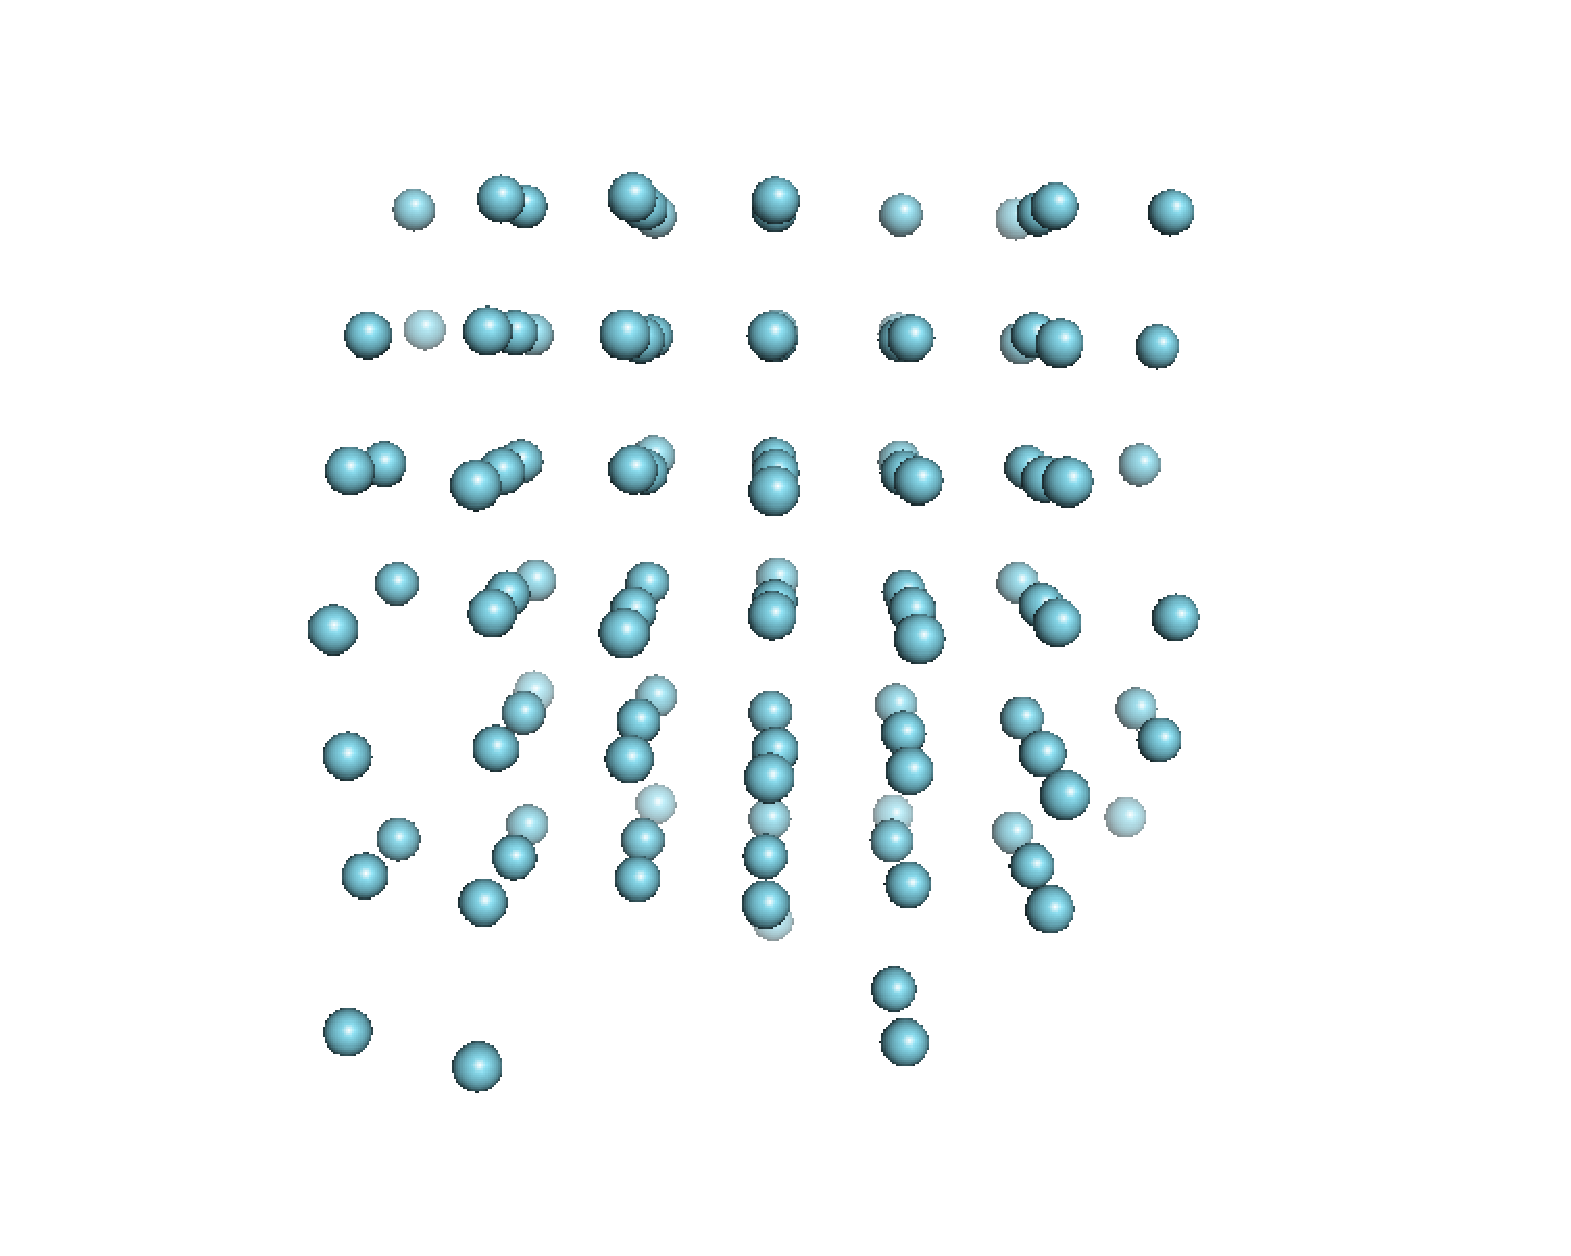
\includegraphics[scale=.25]{ar108scalet4000.pdf}
 \label{fig:ar108scaletemp-4000}
}
\subfigure[Configuraci\'on de Ar al finalizar la simulaci\'on.]
{
 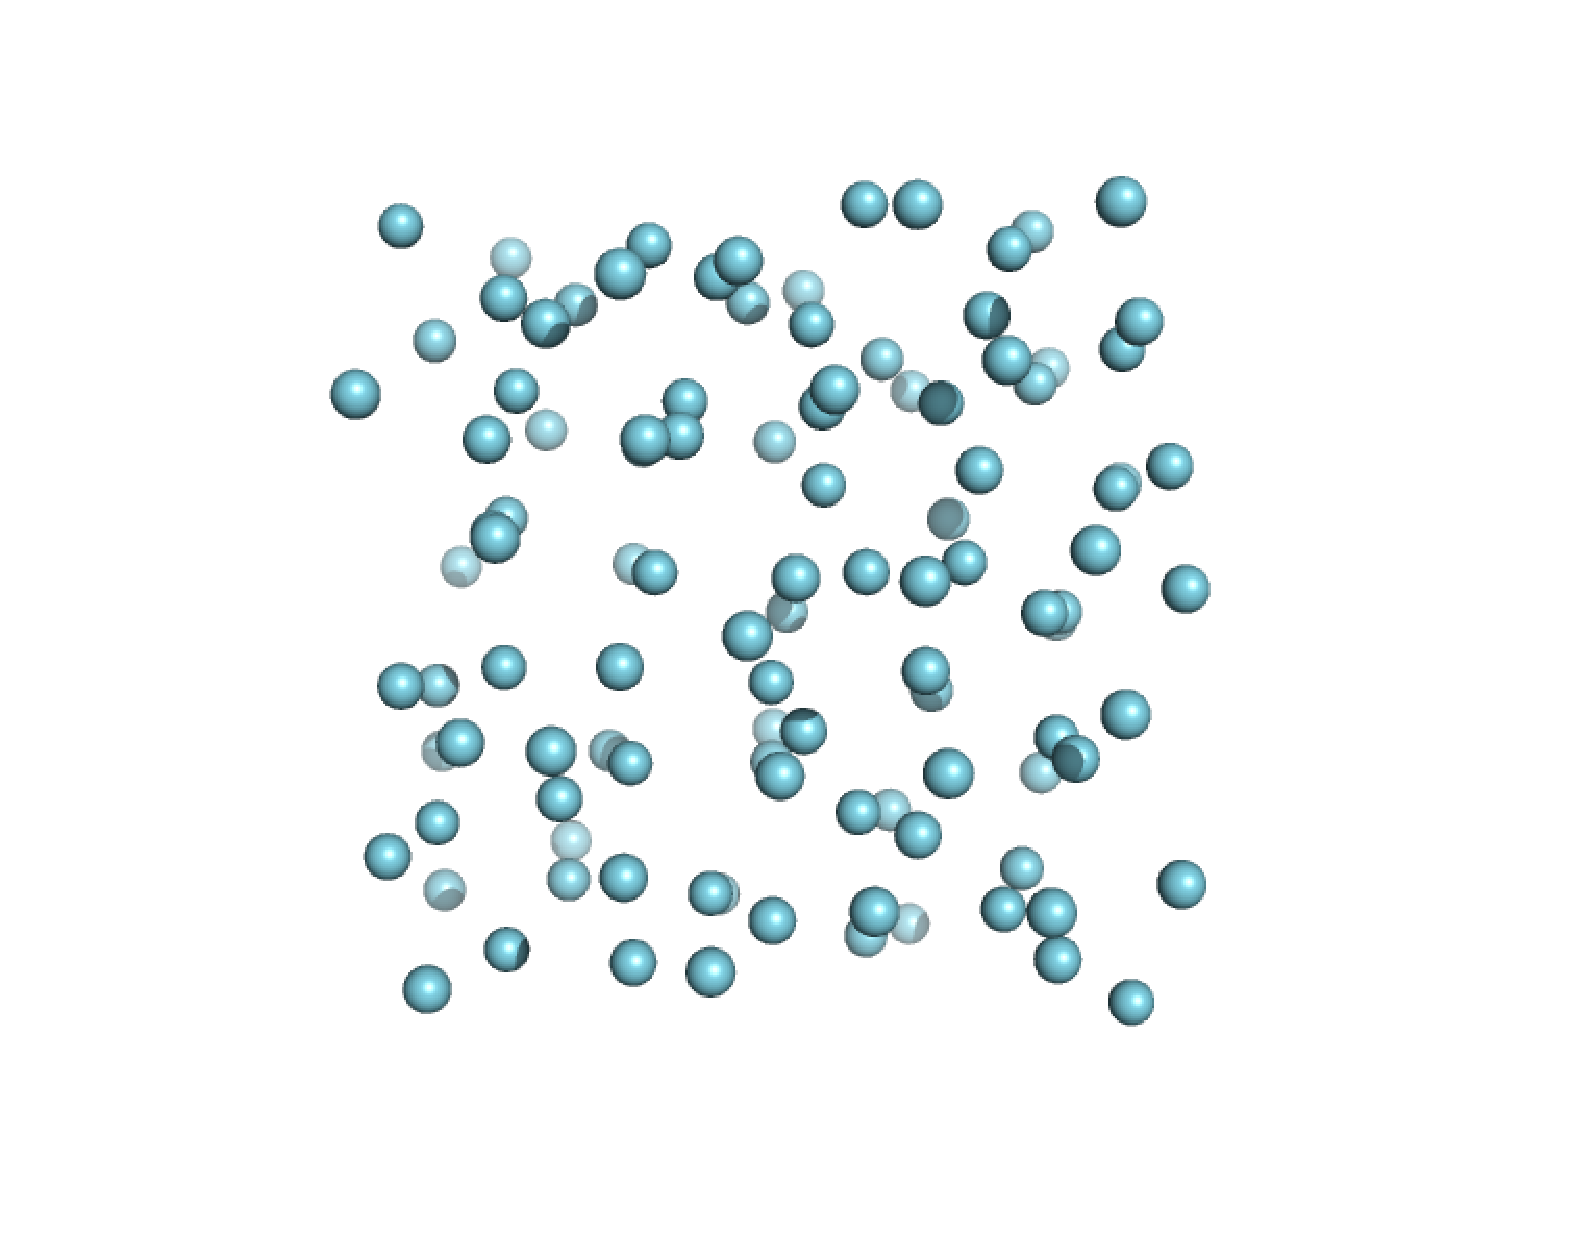
\includegraphics[scale=.25]{ar108scalet15000.pdf}
 \label{fig:ar108scaletemp-15000}
}
\caption{Distintos pasos de una simulaci\'on de din\'amica molecular de 108 \'atomos de Argon.}
\label{fig:ar108scaltemp}
\end{figure}

Adem\'as de este escalamiento de temperatura cl\'asico, {\lpmd} posee dentro de sus plugins otros termostatos, refi\'erase al cap\'itulo~\ref{chap:modulos}.

\subsection{Ejemplo3: Escalamiento de Celda.}

Modificaremos las caracter\'isticas de la celda durante la simulaci\'on, para ello haremos uso del m\'odulo cellscaling, y luego veremos c\'omo se modifica la presi\'on del sistema, junto con la temperatura.

De manera similar al ejemplo anterior, se carga un m\'odulo que modifica una propiedad de nuestro sistema, para llevarlo a las condiciones deseadas. En el siguiente fichero de control, se ve c\'omo se escala una celda.

\begin{multicols}{2}
\setlength{\columnseprule}{.5pt}
\begin{verbatim}
# System file of Ar gas 
# using LPMD
#
###################
#CELL and IN/OUT###
###################
cell crystal a=17.1191 b=17.1191 \
     c=17.1191 alpha=90.0 \
     beta=90.0 gamma=90.0

input module=lpmd file=Ar108.lpmd
output module=xyz file=output.xyz \
     each=20 level=0
###################
#GENERAL###########
###################
prepare temperature t=84
steps 15000
periodic true true true
monitor start=0 end=15000 each=10 \
  properties=step,kinetic-energy, \
  potential-energy,total-energy, \
  temperature,pressure,volume \
  output=monitor.dat
###################
#MODULES DEF#######
###################
use lennardjones as lj_Ar
    sigma 3.41
    epsilon 0.0103408
    cutoff 8.5
enduse

use beeman
    dt 10.0
enduse

use minimumimage
    cutoff 8.5
enduse

use cellscaling as CS
    axis all
    percent 2
    constant true
enduse
###################
#MOD APPLICATION###
###################
potential lj_Ar Ar Ar
integrator beeman
cellmanager minimumimage
apply CS start=5000 end=10000 each=200
\end{verbatim}
\end{multicols}

Podemos ver entonces, c\'omo cambia la presi\'on y el volumen durante la simulaci\'on en las figuras~\ref{fig:ar108scalecpres} y~\ref{fig:ar108scalecvol}, con estos datos se pueden obtener distintos tipos de propiedades mec\'anicas de los materiales en estudio, por ejemplo el m\'odulo de \textit{Bulk}.

\begin{figure}[h!]
\centering
\subfigure[Cambio de Presi\'on en el tiempo.]
{
 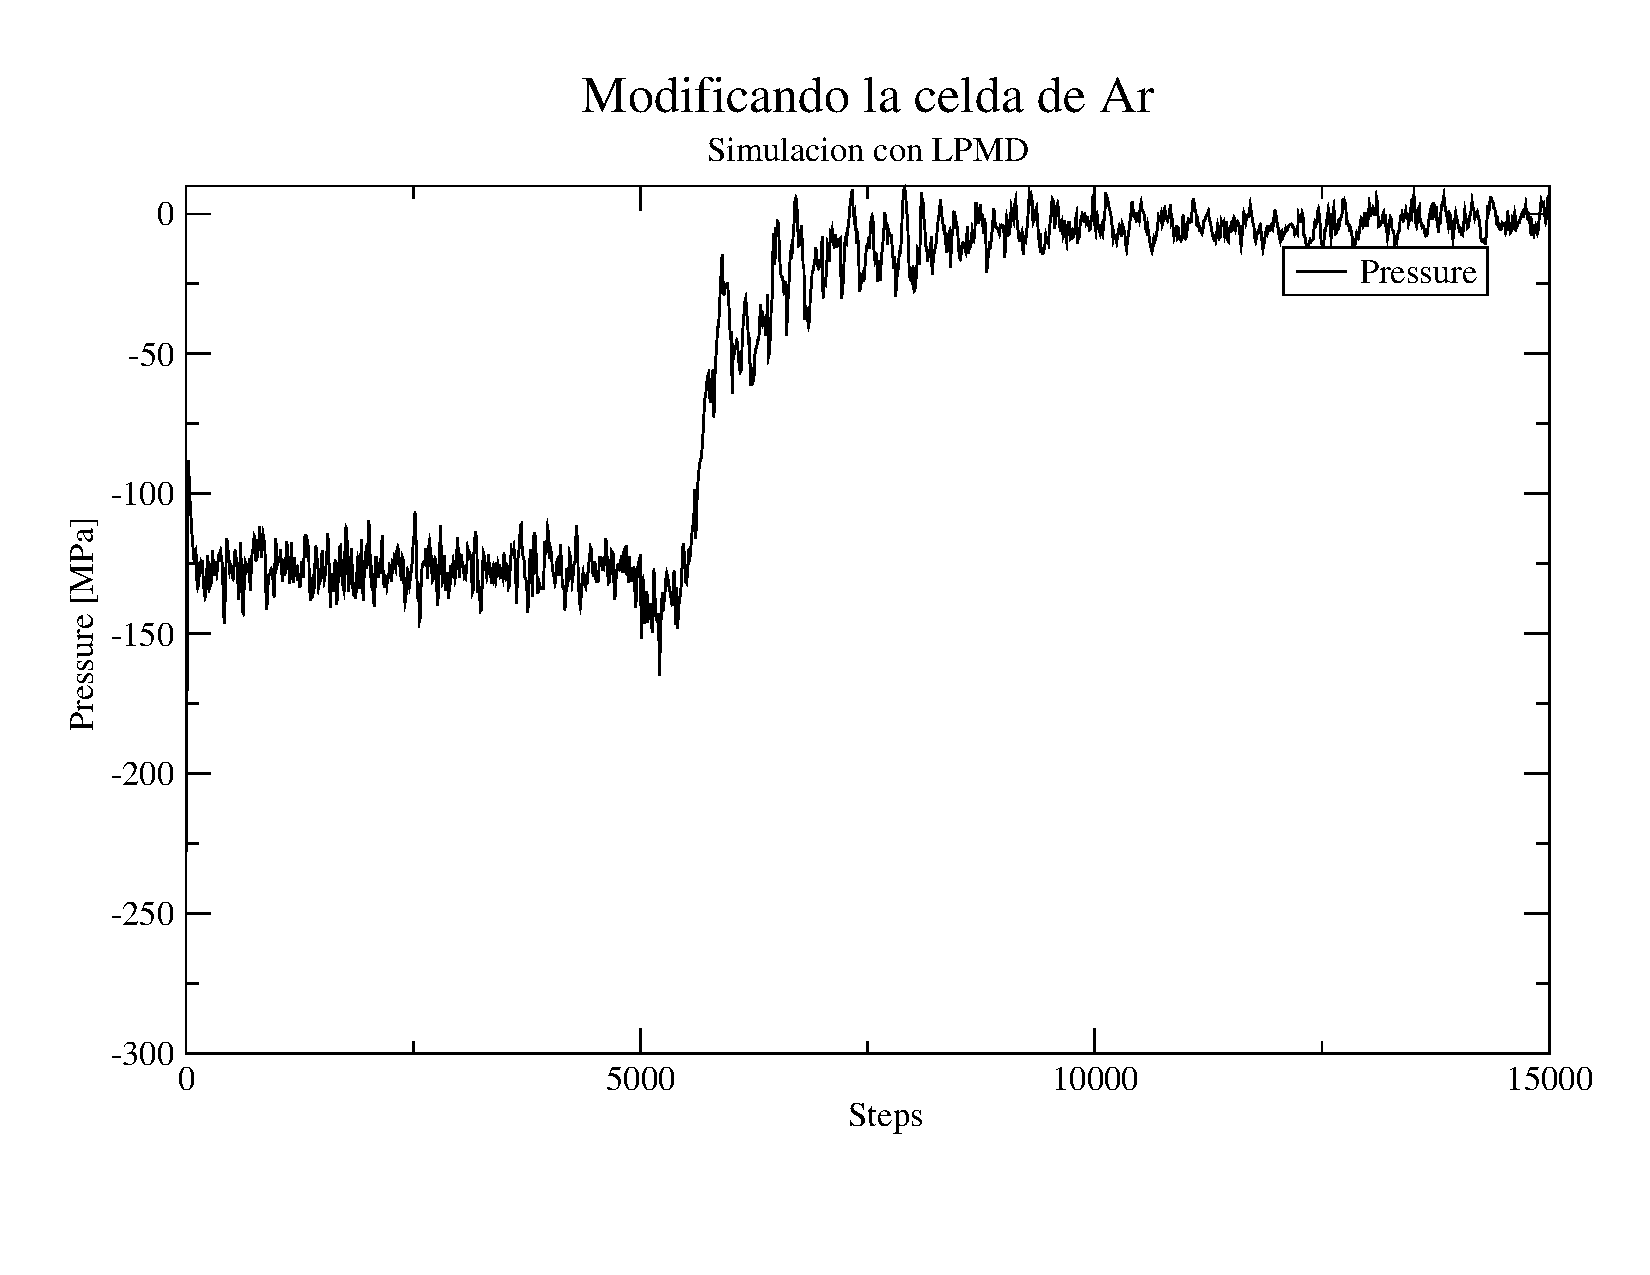
\includegraphics[scale=.25]{ar108scalecpres.pdf}
 \label{fig:ar108scalecpres}
}
\subfigure[Cambio de vol\'umen de la celda durante la simulaci\'on.]
{
 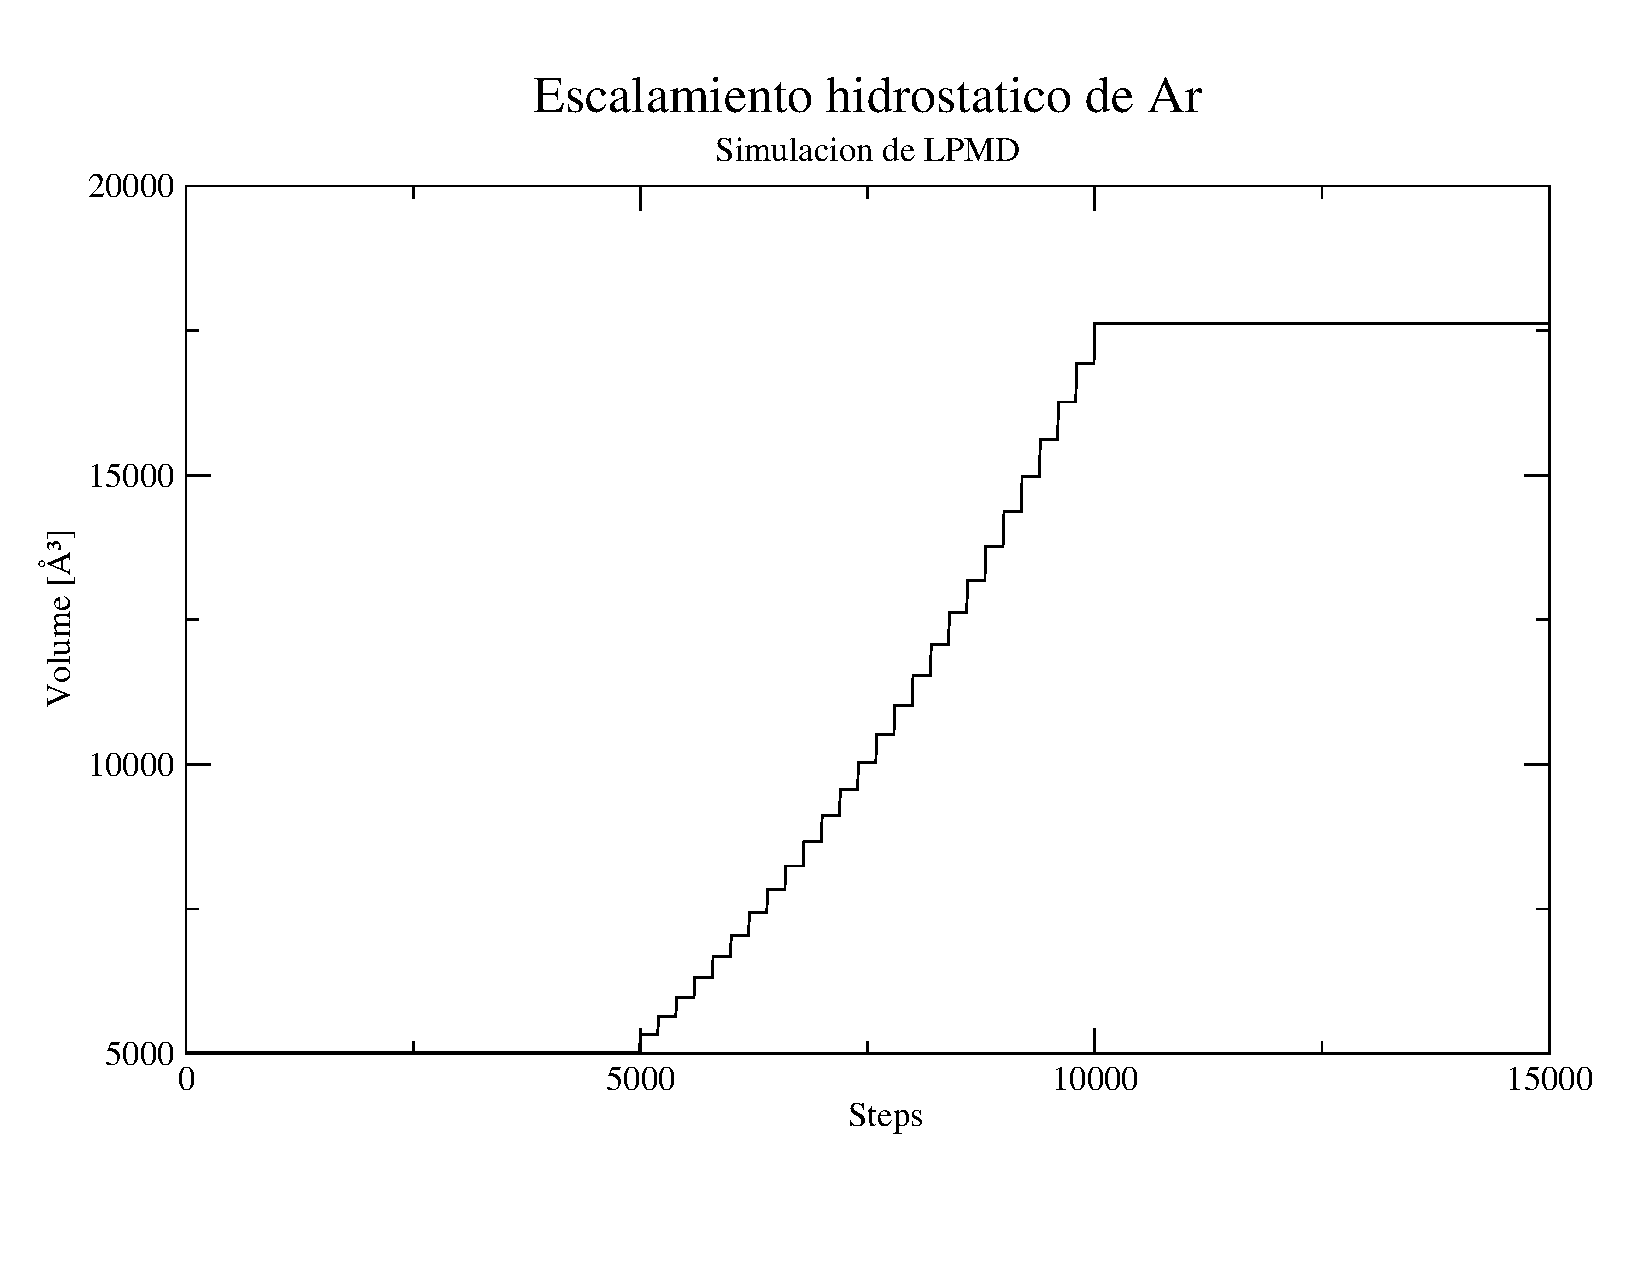
\includegraphics[scale=.25]{ar108scalecvol.pdf}
 \label{fig:ar108scalecvol}
}
\caption{Distintas propiedades del sistema, obtenidas durante la simulaci\'on.}
\label{fig:ar108scalec}
\end{figure}


\subsection{Ejemplo4: Calculando Propiedades durante la Simulaci\'on.}

A continuaci\'on, realizaremos un procedimiento simple de din\'amica molecular, pero esta vez, con una celda de Oro, sobre la cual calcularemos propiedades durante la simulaci\'on. Las propiedades evaluadas ser\'an la \textit{funci\'on de distribuci\'on radial y angular},  y el \textit{n\'umero de coordinaci\'on}. 

\fb{http://www.gnm.cl/software/lpmd/examples/au-prop.tgz}

\begin{multicols}{2}
\setlength{\columnseprule}{.5pt}
\begin{verbatim}
cell crystal a=16.320 b=16.320 \
 c=16.320 alpha=90.0 beta=90.0 \
 gamma=90.0

input module=xyz file=au-input.xyz\
      level=1 inside=true
output module=xyz \
      file=au-output.xyz each=30 \
      level=1

# Periodicity in x, y, z 
periodic true true true

# Molecular dynamics settings
steps 20000

monitor start=0 end=20000 each=1 \
      properties=kinetic-energy,\
      potential-energy,\
      total-energy,temperature \
      output=monitor-cell.out
monitor start=0 end=20000 each=1 \
      properties=virial-pressure,\
      kinetic-pressure,pressure,\
      volume,sxx,syy,szz \
      output=monitor-pres.out

# Using LSC parameters for gold
use suttonchen as sc
    e 0.013
    n 10
    a 4.08
    m 8
    c 34.408
    cutoff 7.2
enduse

use velocityverlet
    dt 1.0
enduse

use linkedcell
	nx 2
	ny 2
	nz 2
	cutoff 8
enduse

use gdr
 rcut 10.0
 bins 200
 output gdr.dat
 average true
enduse

use angdist
 bins 200
 atoms 1 Au
 rcut Au Au 3.4
 output angdist.dat
 average true
enduse

use cordnumfunc
 bins 200
 atoms 1 Au
 rcut 10
 output cordnumfunc.dat
 average true
enduse

potential sc Au Au
cellmanager linkedcell
integrator velocityverlet
property gdr start=10000 \
         end=15000 each=50
property angdist start=10000\
         end=15000 each=50
property cordnumfunc start=10000\
         end=15000 each=50
\end{verbatim}
\end{multicols}

Las propiedades calculadas se pueden observar en las figuras ~\ref{fig:augdr}, ~\ref{fig:aunang} y ~\ref{fig:aucnf}.

\begin{figure}[h!]
\centering
\subfigure[Funci\'on $g(r)$ para celda de Au.]
{
 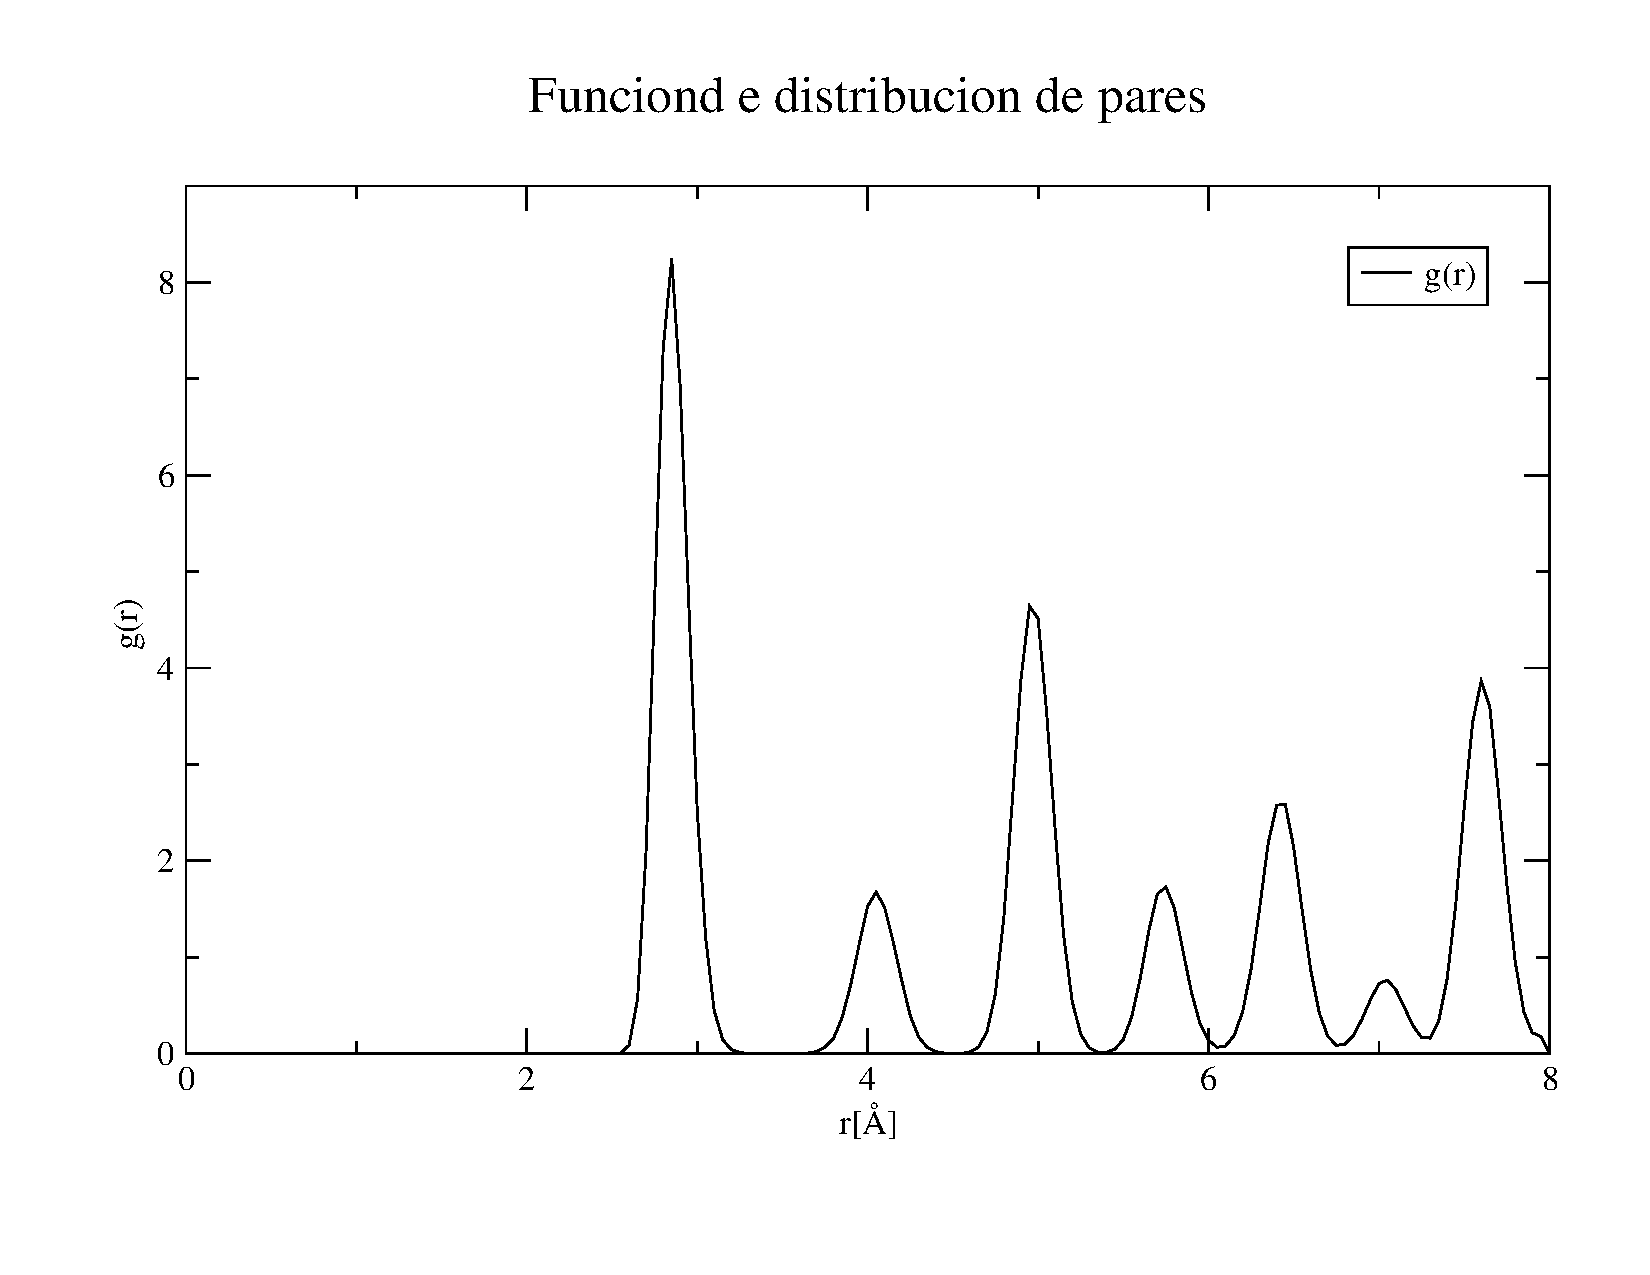
\includegraphics[scale=.25]{augdr.pdf}
 \label{fig:augdr}
}
\subfigure[Funci\'on de distribuci\'on angular.]
{
 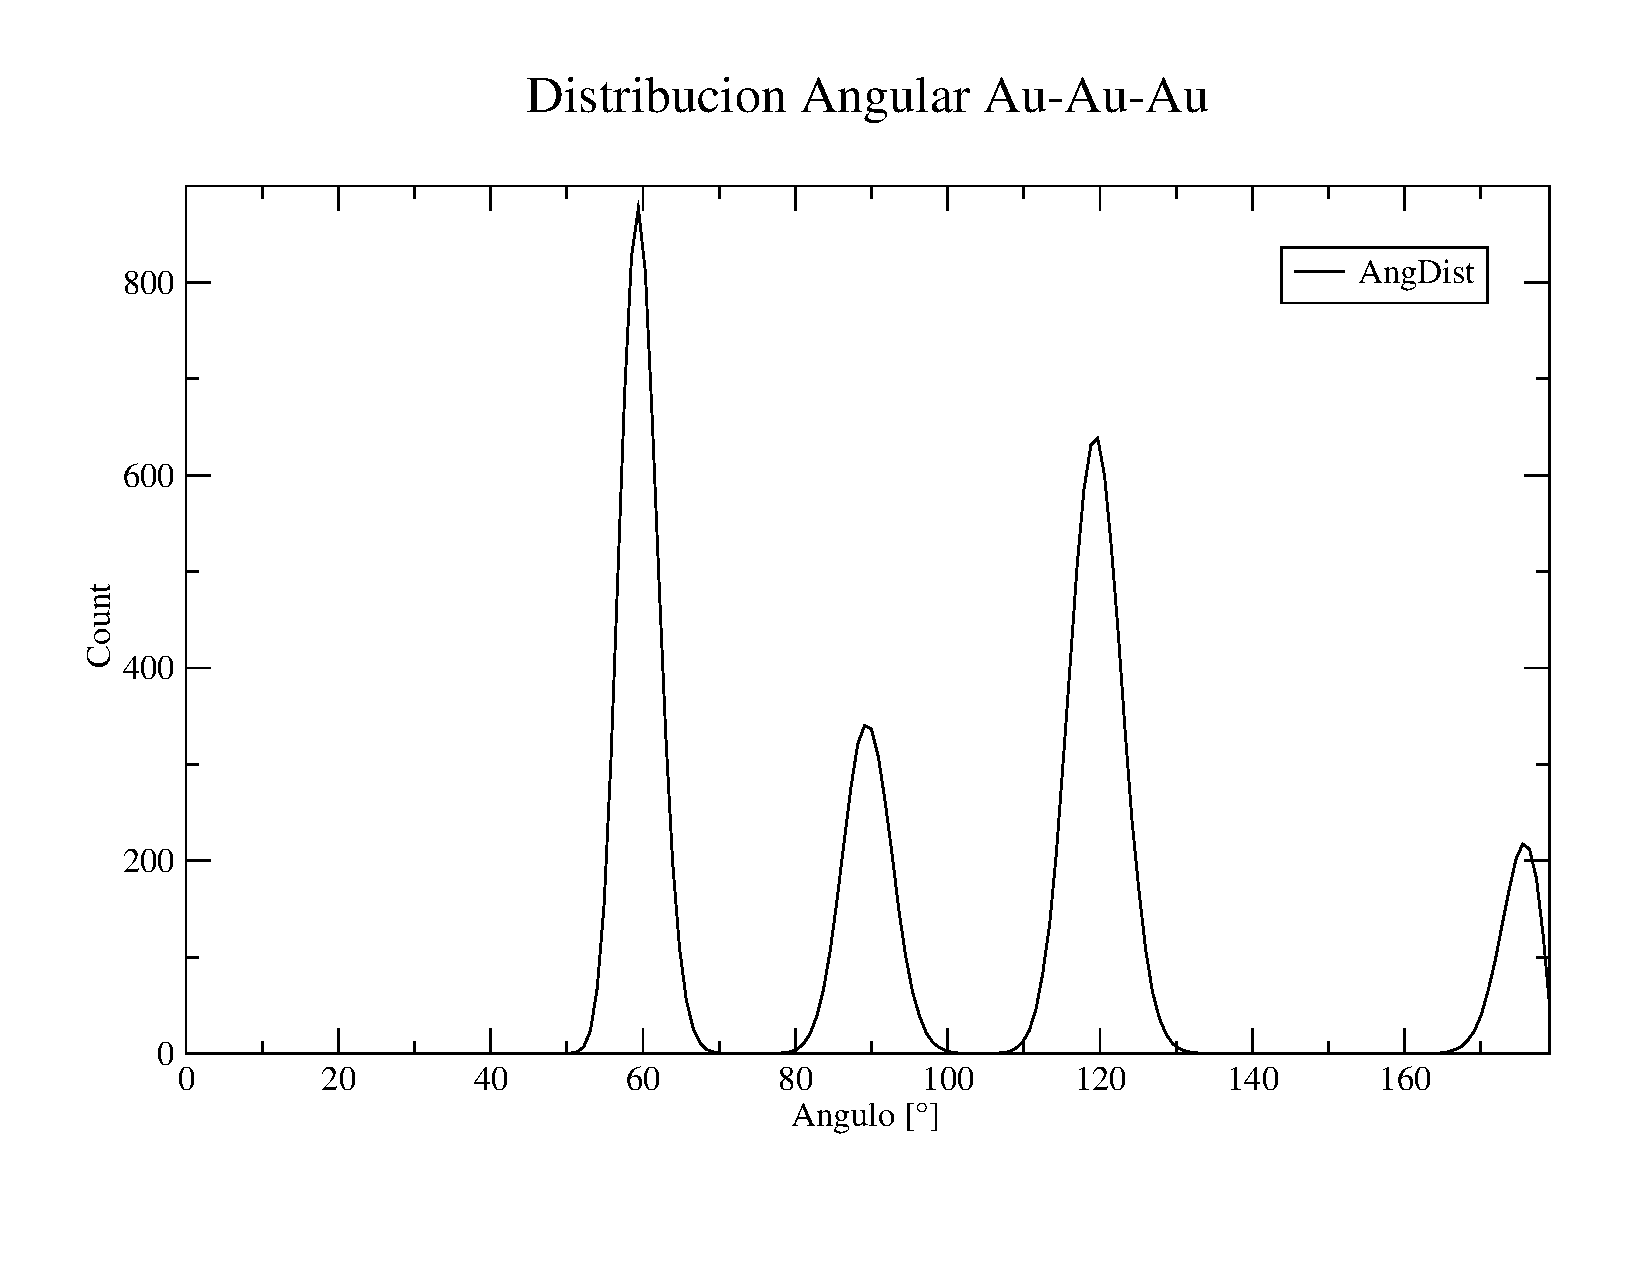
\includegraphics[scale=.25]{aunang.pdf}
 \label{fig:aunang}
}
\subfigure[N\'umero de coordinaci\'on.]
{
 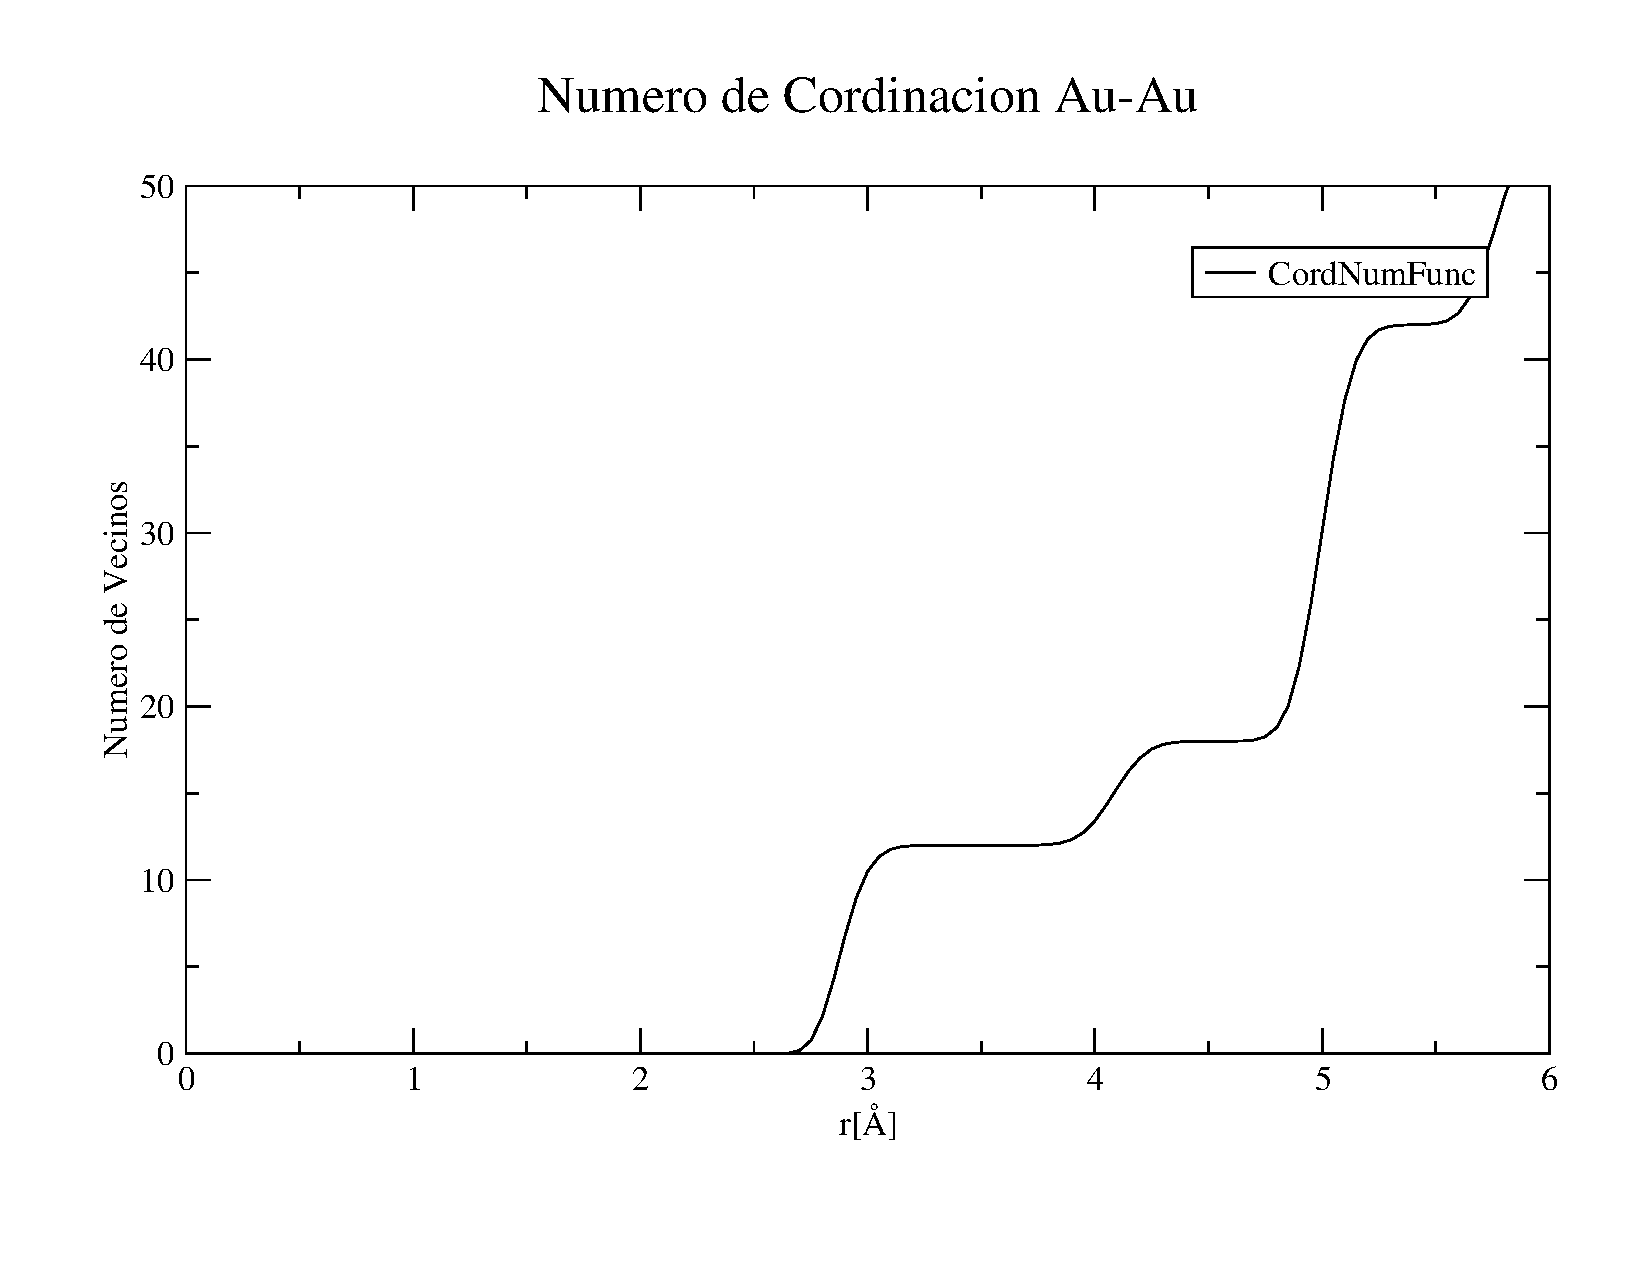
\includegraphics[scale=.25]{aucnf.pdf}
 \label{fig:aucnf}
}
\caption{Propiedades calculadas durante una simulaci\'on de una celda de Au.}
\label{fig:auprop}
\end{figure}



\subsection{Ejemplo5: M\'ultiples corridas con bash.}

Haremos a continuaci\'on un peque\~no estudio de un gas de Ar a distintas temperaturas, para ello nos respaldaremos de los flags del comando {\lpmd} para poder modificar variables a partir de un fichero de control, realizaremos un estudio de la \textit{funci\'on de distribuci\'on de pares} para arg\'on bajo distintas temperaturas.

Las temperaturas iniciales que se utilizar\'an son de 5, 100 y 200 Kelvin, estas tres simulaciones podemos realizarlas a partir de un solo fichero de control, como el que se ve a continuaci\'on:

\begin{multicols}{2}
\setlength{\columnseprule}{.5pt}
\begin{verbatim}
# System file of Ar gas 
# using LPMD
###################
#CELL and IN/OUT###
###################
cell crystal a=17.1191 b=17.1191 \
     c=17.1191 alpha=90.0 \
     beta=90.0 gamma=90.0
input module=lpmd file=Ar108.lpmd
output module=xyz \
     file=output-$(INITIALTEMP).xyz \
     each=20 level=0
###################
#GENERAL###########
###################
prepare temperature t=$(INITIALTEMP)
steps 15000
periodic true true true

monitor start=0 end=15000 each=10 \
  properties=step,kinetic-energy, \
  potential-energy,total-energy, \
  temperature,pressure,volume \
  output=monitor-$(INITIALTEMP).dat
###################
#MODULES DEF#######
###################
use lennardjones as lj_Ar
    sigma 3.41
    epsilon 0.0103408
    cutoff 8.5
enduse

use beeman
    dt 10.0
enduse

use minimumimage
    cutoff 8.5
enduse

use gdr
 bins 200
 rcut 20
 output gdr-$(INITIALTEMP).dat
 average true
enduse
###################
#MOD APPLICATION###
###################
potential lj_Ar Ar Ar
integrator beeman
cellmanager minimumimage
property gdr start=10000 \\
   end=15000 each=30
\end{verbatim}
\end{multicols}

Esta configuraci\'on generar\'a archivos \verb|monitor|, \verb|output| y \verb|gdr| de forma independiente para cada una de las temperaturas, para correrlo basta con :

\begin{center}
 \texttt{for i in 5 100 200 ; \\do lpmd -O INITIALTEMP=\$i opcion-o.control > simulacion-\$i.info ; done}
\end{center}

Los resultados de la funci\'on radial de distribuci\'on de pares, pueden observarse en las figuras ~\ref{fig:opogdr5}, ~\ref{fig:opogdr100} y ~\ref{fig:opogdr200}, donde se ve claramente que la condici\'on de temperatura inicial es un factor importante en el desarrollo de la din\'amica molecular ya que son las condiciones iniciales con las que comienza el sistema su evoluci\'on.

\begin{figure}[h!]
\centering
\subfigure[Funci\'on $g(r)$ para 5K.]
{
 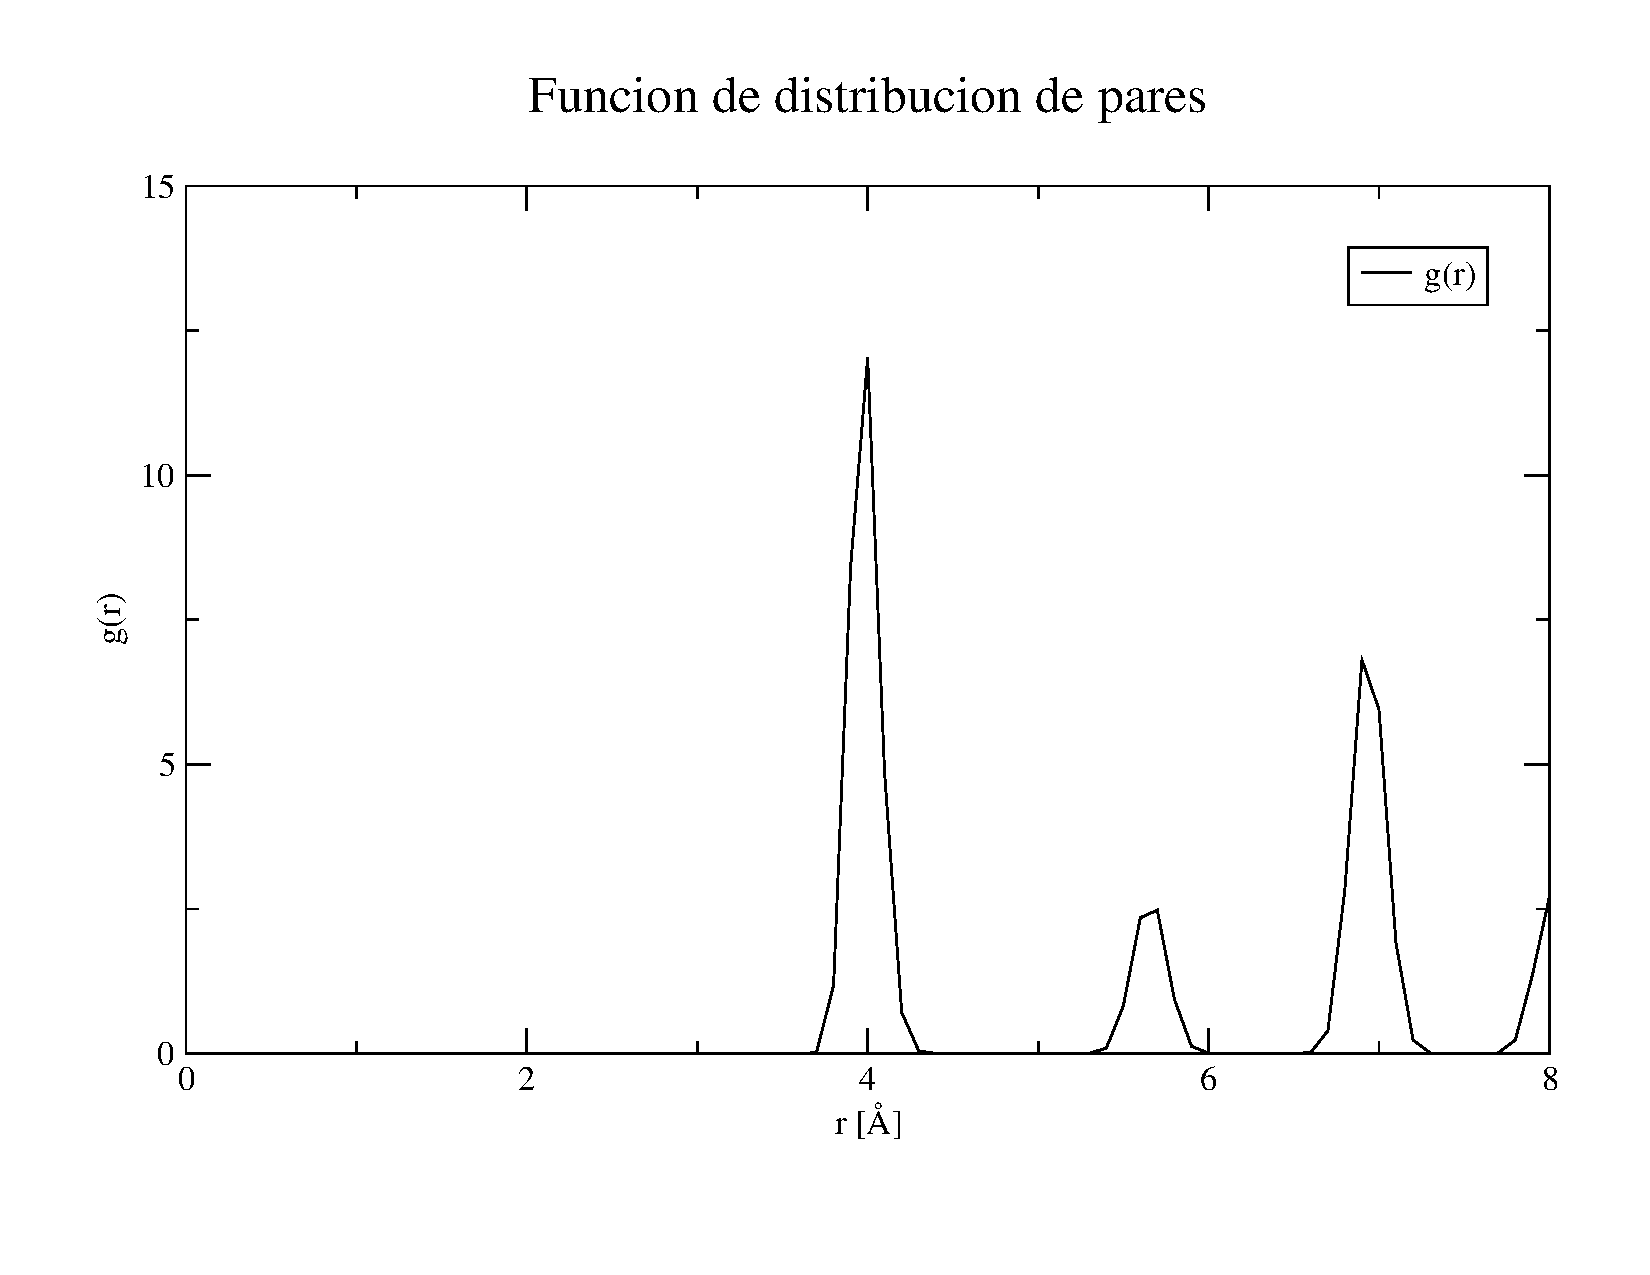
\includegraphics[scale=.25]{opogdr5.pdf}
 \label{fig:opogdr5}
}
\subfigure[Funci\'on $g(r)$ para 100K.]
{
 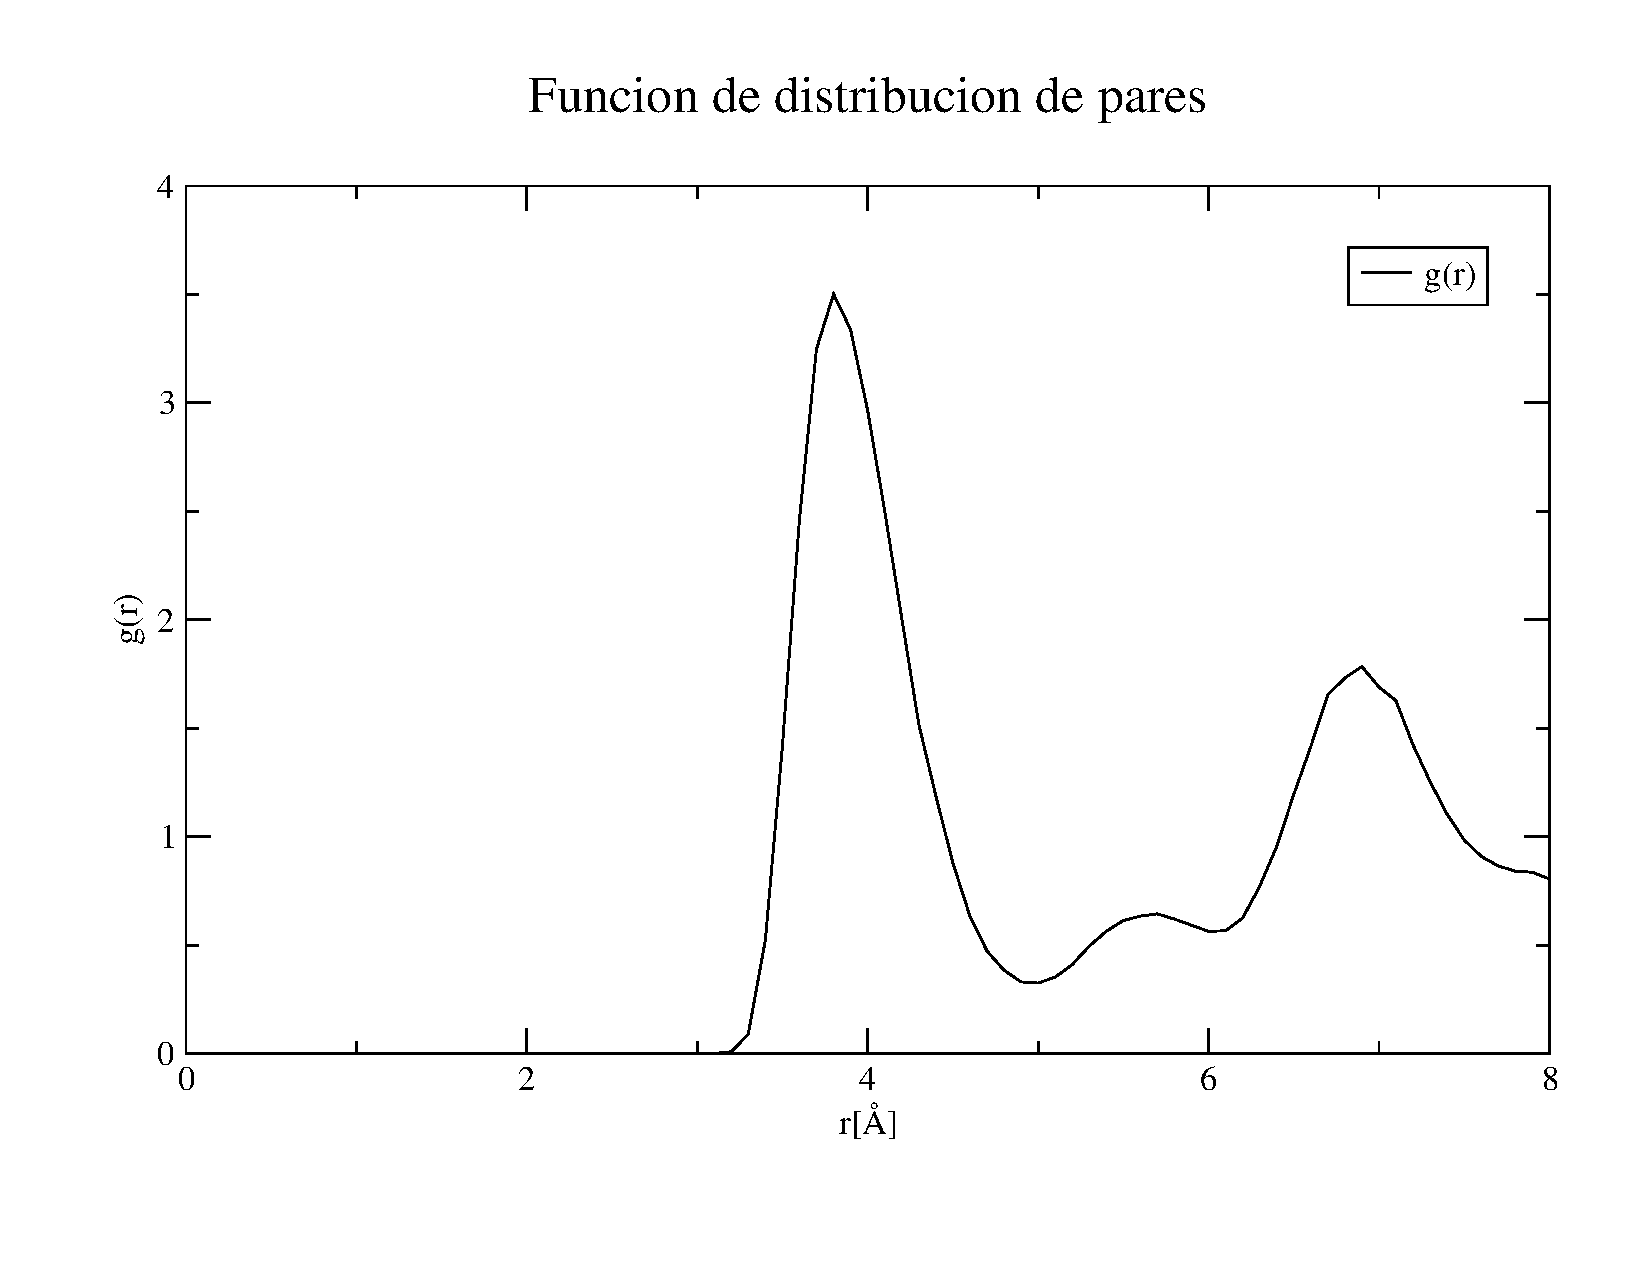
\includegraphics[scale=.25]{opogdr100.pdf}
 \label{fig:opogdr100}
}
\subfigure[Funci\'on $g(r)$ para 200K.]
{
 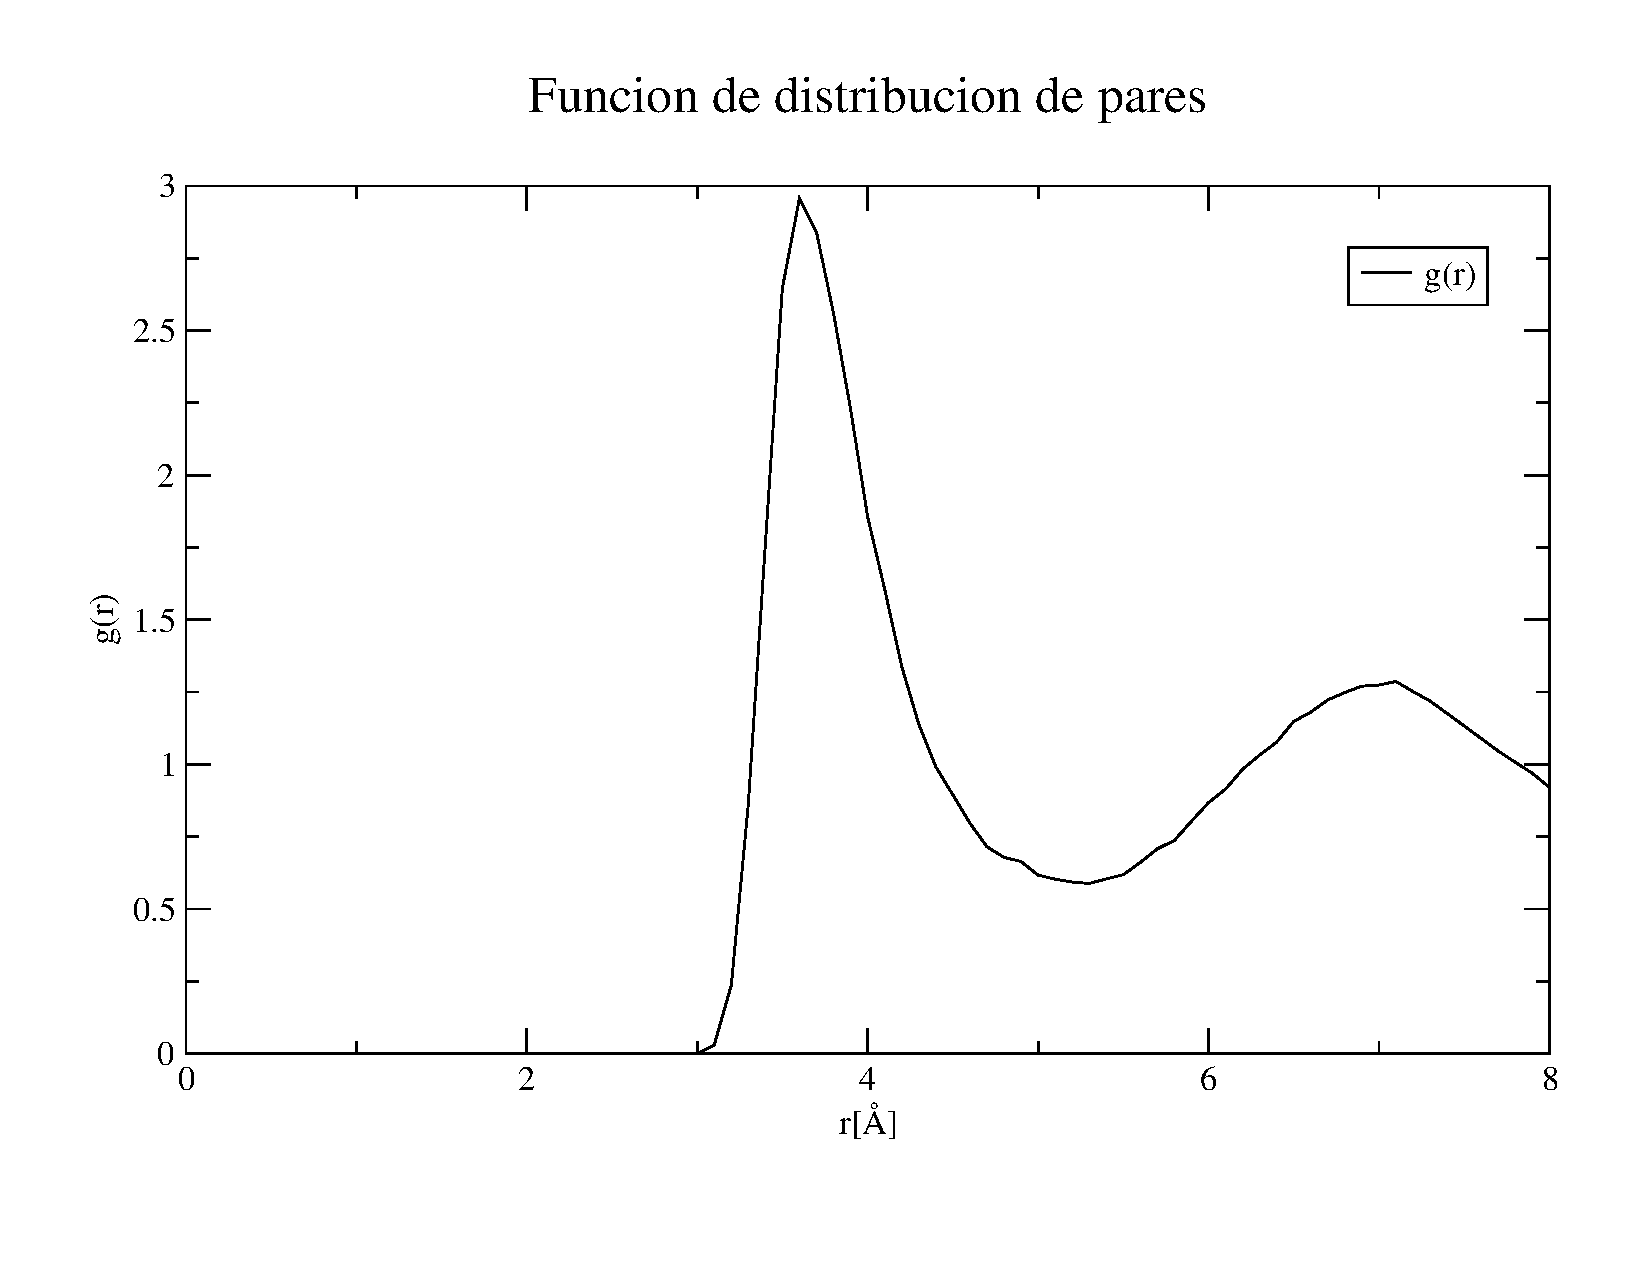
\includegraphics[scale=.25]{opogdr200.pdf}
 \label{fig:opogdr200}
}
\caption{Funci\'on $g(r)$ para distintas temperaturas iniciales del sistema.}
\label{fig:opogdr}
\end{figure}


% \subsection{Ejemplo6: Generando ficheros pov para crear pel\'iculas.}
% 
% Fue uno de los primeros \textit{approach} a lo que a m\'odulos de visualizaci\'on se refiere, su intenci\'on es generar, a partir de la simulaci\'on, un set de ficheros \verb|pov| para un posterior renderizado y creaci\'on de peliculas, animaciones o simplemente imagnes de alta calidad. El ejemplo puede descargarse en:
% 
% \fb{http://wwww.gnm.cl/software/lpmd/examples/arpovmul.tgz}
% 
% Veamos a continuacion el c\'odigo utilizado para la simulaci\'on:
% 
% \begin{multicols}{2}
% \setlength{\columnseprule}{.5pt}
% \begin{verbatim}
% # System file of Ar gas 
% # using LPMD
% #
% ###################
% #CELL and IN/OUT###
% ###################
% cell crystal a=17.1191 b=17.1191 \
%    c=17.1191 alpha=90.0 beta=90.0 \
%    gamma=90.0
% 
% input module=lpmd file=Ar108.lpmd
% output module=xyz file=output.xyz \
%    each=20 level=0
% ###################
% #GENERAL###########
% ###################
% prepare replicate 2 2 2
% prepare temperature 84
% charge Ar 0.0
% steps 10
% dumping file=ljargon.dump each=5
% periodic true true true
% 
% #Cargamos inmediatamente pressure
% #para poder visualizar con monitor
% 
% use pressure
% enduse
% 
% monitor start=0 end=5000 each=10 \
%   properties=kinetic-energy, \
%   potential-energy,total-energy, \
%   pressure,volume output=monitor.dat
% ###################
% #MODULES DEF#######
% ###################
% use lennardjones as lj_Ar
%     sigma 3.41
%     epsilon 0.0103408
%     cutoff 8.5
% enduse
% 
% use beeman
%     dt 10.0
% enduse
% 
% use minimumimage
%     cutoff 8.5
% enduse
% 
% use povray
%     header shoot-
%     direct movie
%     text "Modelacion de Ar" <dl> \
%       <green> [3] ()
%     text " Step = % " <uc> <red> [3] \
%       (Step)
%     rotate <0,45,0>
%     background <1,1,1>
% enduse
% 
% ###################
% #MOD APPLICATION###
% ###################
% potential lj_Ar Ar Ar
% integrator beeman
% cellmanager minimumimage
% visualize povray start=0 \
%    end=10 each=1
% \end{verbatim}
% \end{multicols}
% 
% %El resultado de la simulaci\'on es la generaci\'on de ficheros \verb|pov| que se encuentran dentro del directorio \verb|movie|, es importante destacar que la conversion de estos ficheros \verb|pov| en im\'agenes de alta calidad, puede llevarse a cabo con \verb|povray|, un software libre de renderizado de imagenes. Un resultado de la conversi\'on de una im\'agen pude verse en la figura~\ref{fig:povrayex}
% 
% \begin{figure*}[h!]
% \begin{minipage}{8cm}
%  El resultado de la simulaci\'on es la generaci\'on de ficheros \verb|pov| que se encuentran dentro del directorio \verb|movie|, es importante destacar que la conversion de estos ficheros \verb|pov| en im\'agenes de alta calidad, puede llevarse a cabo con \verb|povray|, un software libre de renderizado de imagenes. Un resultado de la conversi\'on de una im\'agen pude verse en la figura~\ref{fig:povrayex}
% \end{minipage}
% \hfill
% \begin{minipage}{7cm}
% \centering
%  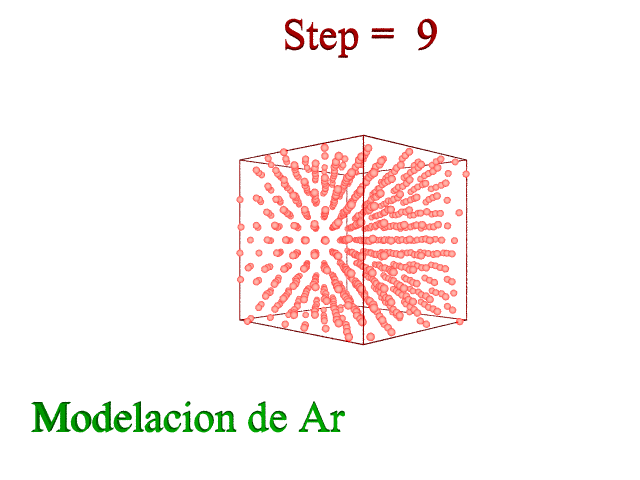
\includegraphics[scale=.3]{shoot-pov.png}
% \caption{Im\'agen resultante de los ficheros \texttt{pov} generados en la simulaci\'on.}
% \label{fig:povrayex}
% \end{minipage}
% \end{figure*}

% \subsection{Cambiando el integrador durante la simulaci\'on.}
% 
% Una caracter\'istica de {\lpmd} es poder cambiar el integrador, durante la simulaci\'on, esto es utilizado en un ejemplo a continuaci\'on que puede descagar en:
% 
% \fb{http://wwww.gnm.cl/software/lpmd/examples/int-change.tgz}
% 
% \subsection{Calculo de Modulo de Bulk}
% 
% En este ejemplo, se calcula el m\'odulo de Bulk para Au modificando el tama\~no de la celda de forma hidrostatica durante la simulaci\'on, para as\'i obtener directamente las presiones.

%%%%%%%%%%%%%%%%%%%%%%%%%%%%%%%%%%%%%%%%%%%%%%%%%%%%%%%%%%%%%%%%%
%%%%%%%%%%%%%%%%%%%%%%%%%%%%%%%%%%%%%%%%%%%%%%%%%%%%%%%%%%%%%%%%%
\section{Ejemplos LPMD-ANALYZER}

La funci\'on principal de \textbf{lpmd-analyzer} es poder cargar configuraciones, provenientes de archivos con distintas extensiones, tales como \verb|xyz| o \verb|lpmd|, para poder obtener an\'alisis de estas configuraciones.

Para los ejemplos de \textbf{lpmd-analyzer} utilizaremos un fichero de tipo \verb|xyz| proveniente de una simulaci\'on de din\'amica molecular hecha con \textbf{moldy} de di\'oxido de germanio, o germania, como se ve en la figura~\ref{fig:geo2-1}.

La manera de utilizar \textbf{lpmd-analyzer} es ejecutando \verb|lpmd-analyzer archivo.control|.

\cajafi{geo2-1.pdf}{Una de las configuraciones de GeO$_2$ bajo condiciones ambientales, del total de configuraciones obtendremos distintas propiedades utilizando \textbf{lpmd-analyzer}.}{geo2-1}


\subsection{Ejemplo1: Calculando la Funci\'on Radial de Distribuci\'on.}

Para calcular la funci\'on de distribuci\'on radial $g(r)$, creamos un fichero de \verb|control| tomando como input un archivo \verb|xyz| que contiene 101 configuraciones de 576 \'atomos, pero a diferencia de los ficheros de control de {\lpmd}, este fichero cuenta s\'olo con lo necesario para evaluar una propiedad, como se ve a continuaci\'on:

\begin{multicols}{2}
\setlength{\columnseprule}{.5pt}
\begin{verbatim}
#Fichero que calcula g(r)
#para un fichero xyz con 101 
#configuraciones

cell cubic a=20.7
input module=xyz file=final20p8.xyz \
      inside=true

use lcbinary
   mode auto
   cutoff 10
enduse

use gdr as pgdr
   bins 200
   rcut 10
   output gdr.dat
   average true
enduse

cellmanager lcbinary
property pgdr start=0 end=100 each=1
\end{verbatim}
\end{multicols}

La manera en que se debe correr este archivo de control es ejecutando \verb|lpmd-analyzer gdr.control|. La informaci\'on del $g(r)$ ser\'a guardada en el fichero \verb|gdr.dat| el cual entregar\'a s\'olo un $g(r)$ obtenido a partir del promedio de los $g(r)$ de cada configuraci\'on. El resultado final del c\'alculo de $g(r)$ se puede ver en la figura~\ref{fig:exagdr}.

\cajafi{gdr.pdf}{Funci\'on radial de distribuci\'on de pares, note que \texttt{lpmd-analyzer}, autom\'aticamente calcula para cada una de las especies at\'omicas de la muestra y para el total.}{exagdr}

\subsection{Ejemplo2: Desplazamiento Cuadr\'atico Medio.}

Calcularemos ahora el desplazamiento cuadr\'atico medio (\verb|msd|) de nuestra muestra, utilizando el m\'odulo \verb|msd|. El archivo de control, se muestra a continuaci\'on:

\begin{multicols}{2}
\setlength{\columnseprule}{.5pt}
\begin{verbatim}
#Fichero que calcula el msd
#para un fichero xyz con 101 
#configuraciones

cell cubic a=20.7
input module=xyz file=final20p8.xyz \
      inside=true

use lcbinary
    mode auto
    cutoff 10
enduse

use msd as pmsd
   output msd.dat
enduse

cellmanager lcbinary
property pmsd start=0 end=100 each=1
\end{verbatim}
\end{multicols}

\cajafi{msd.pdf}{Desplazamiento cuadr\'atico medio (\texttt{msd}) calculado con \texttt{lpmd-analyzer}.}{examsd}

La informaci\'on obtenida del fichero de salida \verb|msd.dat| se puede ver en la figura~\ref{fig:examsd}.

\subsection{Ejemplo3: Calculando la Distribuci\'on Angular.}

Para calcular la distribuci\'on angular crearemos el siguiente fichero de control:

\begin{multicols}{2}
\setlength{\columnseprule}{.5pt}
\begin{verbatim}
#Calcula distribucion angular
#para un fichero xyz con 101 
#configuraciones

cell cubic a=20.7

input module=xyz file=final20p8.xyz /
      inside=true

use lcbinary
    mode auto
    cutoff 10
enduse

use angdist as ang
   bins 200
   atoms 2 Ge O
   rcut Ge Ge 3.6
   rcut Ge O  1.9
   rcut O  O  3.2
   output ang.dat
   average true
enduse

cellmanager lcbinary
property ang start=0 end=100 each=1
\end{verbatim}
\end{multicols}

El resultado de las distribuciones angulares de toda la muestra se ven en la figura~\ref{fig:exaang}, los radios de corte utilizados corresponden, como en muchos de los an\'alisis de este tipo, al primer m\'inimo despu\'es del primer \textit{peak} de la funci\'on radial de distribuci\'on de pares.

\cajafi{ang.pdf}{Distribuci\'on angular para toda la muestra, calculada con \texttt{lpmd-analyzer}.}{exaang}

\subsection{Ejemplo4: N\'umero de Coordinaci\'on.}

El n\'umero de coordinaci\'on puede ser calculado de distintas formas, en esta ocasi\'on, haremos uso de la funci\'on n\'umero de coordinaci\'on para el c\'alculo.

\begin{multicols}{2}
\setlength{\columnseprule}{.5pt}
\begin{verbatim}
#Calcula numero de coordinacion
#para un fichero xyz con 101
#configuraciones

cell cubic a=20.7

input module=xyz \
      file=final20p8.xyz \
      level=0 inside=true

use lcbinary
    mode auto
    rcut 10 
enduse

use cordnumfunc as cnf
  bins 200
  atoms 2 Ge O
  rcut 10
  output cnf.dat
  average true
enduse

cellmanager lcbinary
property cnf start=0 end=100 each=1
\end{verbatim}
\end{multicols}

Podemos ver el resultado del n\'umero de coordinaci\'on en la figura~\ref{fig:exacnf}.

\cajafi{cnf.pdf}{Algunos resultados del n\'umero de coordinaci\'on calculados con \texttt{lpmd-analyzer}.}{exacnf}

% \subsection{Distribuci\'on de velocidades.}
% La dsitribuci\'on de velocidades corresponde a la forma en que las velocidades de las especies at\'omicas estan distribuidas, en este caso, el archivo de control queda de la forma:
% 
% \begin{multicols}{2}
% \setlength{\columnseprule}{.5pt}
% \begin{verbatim}
% #Calcula numero de distribucion 
% #de velocidades
% 
% cell cubic a=20.7
% 
% input module=xyz \
%       file=final20p8.xyz \
%       level=0 inside=true
% 
% use linkedcell
%     nx 1
%     ny 1
%     nz 1
%     rcut 20 
% enduse
% 
% use veldist as vdf
%   bins 200
%   output vdf.dat
% enduse
% 
% cellmanager linkedcell
% property vdf start=1 end=100 each=1
% \end{verbatim}
% \end{multicols}


%%%%%%%%%%%%%%%%%%%%%%%%%%%%%%%%%%%%%%%%%%%%%%%%%%%%%%%%%%%%%%%%%
%%%%%%%%%%%%%%%%%%%%%%%%%%%%%%%%%%%%%%%%%%%%%%%%%%%%%%%%%%%%%%%%%
\section{Ejemplos LPMD-CONVERTER}

Pese a que existe una muy amplia variedad de c\'odigos para convertir entre formatos de ficheros, {\lpmd} cuenta con uno propio que, adem\'as de poder convertir entre los formatos seg\'un el m\'odulo, tiene la caracter\'istica de poder modificar la celda, agregando, eliminando o bien seleccionando \'atomos. A continuaci\'on veremos un par de ejemplos simples que pueden realizar con \textbf{lpmd-converter}.

\subsection{Ejemplo1: De un formato a otro}

El siguiente ejemplo, muestra c\'omo convertir un fichero \verb|POSCAR|, que es un fichero de entrada de posiciones at\'omicas para \textbf{vasp}, en un formato de tipo \verb|xyz|.

\begin{multicols}{2}
\setlength{\columnseprule}{.5pt}
\begin{verbatim}
# input para lpmd-converter
cell vector ax=2.650038 ay=0.0 az=0.0 \
     bx=-1.53 by=3.06 bz=0 cx=0.0 \
     cy=0.0 cz=13.45
input module=vasp file=POSCAR \
      species=Ti,Ga,N
# escribe la salida en formato xyz
output xyz file=TiGaN.xyz level=0
\end{verbatim}
\end{multicols}

Obteniendo el resultado, ejecutando \verb|lpmd-converter vasp2xyz.control|.
% Esto mismo se puede ejecutar del terminal sin necesidad de crear un archivo de control, para ello siguiendo los par\'ametros del ejemplo se debe escribir,
% 
% \verb|lpmd-converter |

\subsection{Ejemplo2: Eliminando \'atomos}

Con un archivo de entrada y el plugin \verb|selectatoms|, se pueden seleccionar o modificar \'atomos dentro de una celda de simulaci\'on, es decir, se puede convertir la celda original en una nueva celda modificada. A continuaci\'on modificamos una celda original en formato \verb|xyz| en una nueva celda en la cual hemos eliminado una regi\'on del espacio.

\begin{multicols}{2}
\setlength{\columnseprule}{.5pt}
\begin{verbatim}
# input para lpmd-converter
cell cubic a=20.7
input module=xyz file=final20p8.xyz \
      level=0 inside=true
output module=xyz file=newcell.xyz \
       level=0
filter box x=10-20.7 y=10-20.7 \
z=0-20.7 inverse=true

\end{verbatim}
\end{multicols}

Con el plugin filter se ha seleccionado una parte de la caja, pero, al aplicarle la opci\'on \verb|inverse=true|, se ha seleccionado finalmente lo que quedo fuera de la zona de la caja antes seleccionada, lo cual se muestra en la figura~\ref{fig:selectatoms}. 

\begin{figure}[h!]
\centering
\subfigure[Configuraci\'on at\'omica original.]
{
 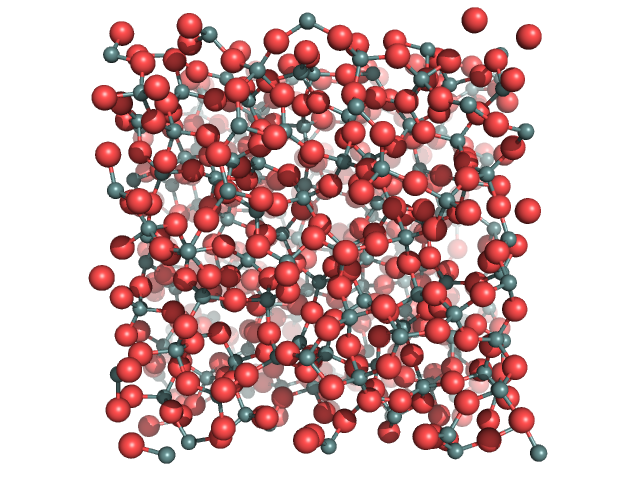
\includegraphics[scale=.25]{GeO2-all.png}
 \label{fig:selectatoms-con}
}
\subfigure[Nueva configuraci\'on at\'omica en la cual se ha eliminado una regi\'on del espacio.]
{
 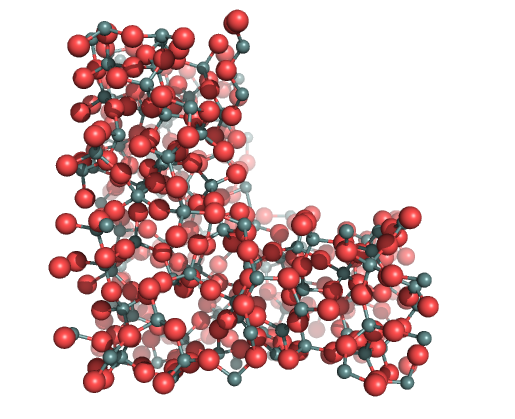
\includegraphics[scale=.30]{GeO2-selat.png}
 \label{fig:selectatoms-sin}
}
\caption{Configuraciones at\'omicas antes y despu\'es de aplicar filter, muy \'util para dise\~nar pel\'iculas con defectos o elementos distintos dentro de una celda, un posterior an\'alisis tambi\'en se puede llevar a cabo por regiones.}
\label{fig:selectatoms}
\end{figure}

%%%%%%%%%%%%%%%%%%%%%%%%%%%%%%%%%%%%%%%%%%%%%%%%%%%%%%%%%%%%%%%%%%%%%%%%%%%%%%%%%%%%%%%%%%%%%%%%%%%%%%%%%
%%%%%%%%%%%%%%%%%%%%%%%%%%%%%%%%%%%%%%%%%%%%%%%%%%%%%%%%%%%%%%%%%%%%%%%%%%%%%%%%%%%%%%%%%%%%%%%%%%%%%%%%%
%CAPITULO 7%%%%%%%%%%%%%%%%%%%%%%%%%%%%%%%%%%%%%%%%%%%%%%%%%%%%%%%%%%%%%%%%%%%%%%%%%%%%%%%%%%%%%%%%%%%%%%
%%%%%%%%%%%%%%%%%%%%%%%%%%%%%%%%%%%%%%%%%%%%%%%%%%%%%%%%%%%%%%%%%%%%%%%%%%%%%%%%%%%%%%%%%%%%%%%%%%%%%%%%%
%%%%%%%%%%%%%%%%%%%%%%%%%%%%%%%%%%%%%%%%%%%%%%%%%%%%%%%%%%%%%%%%%%%%%%%%%%%%%%%%%%%%%%%%%%%%%%%%%%%%%%%%%
%\chapter{Desarrollando M\'odulos}
\label{chap:own}

\section{Idea Principal}

Una de las caracter\'isticas princpales de \lpmd con respecto a otros c\'odigos de Din\'amica Molecular es su gran \textit{modularidad} lo que hace que muchas propiedades de un ciclo regular de din\'amica molecular sean modificables facilmentes, por ejemplo un cilco de din\'amica molecular consta de muchas \textbf{piezas} constantes, tales como los potenciales, integradores o bien una propiedad que puede ser calculada de forma instantanea o que requiere una correlaci\'on temporal del sistema.

Consideremos por ejemplo :

Se puede observar claramente que existen \textbf{bloques} en donde la caracter\'istica principal de cada uno de ellos en \lpmd es que son modificables por diferentes tipos de \textbf{m\'odulos} que \textit{encajan} perfectamente en estos bloques, estos m\'odulos pueden ser din\'amicos lo que da una ventaja significativa a la hora de desarrollar el c\'odigo necesario para trabajar con \'el.

En este cap\'itulo se exponen las distintas piezas \textbf{modificables} de \lpmd que har\'an de este un c\'odigo mucho m\'as \'util para el desarrollo de distintas investigaciones con una misma herramienta.

\section{Desarrollando un Potencial}

Una de las piezas fundamentales en la din\'amica molecular, es la integraci\'on de un potencial interat\'omico entre las particulas que componen el sistema, es por eso que \lpmd facilita 

\section{Desarrollando una Propiedad}

Durante una simulaci\'on de din\'amica molecular una de las herramientas m\'as utilizadas  son las propiedades f\'isicas del sistema, las que son, een ocaciones, comparables con resultados experimentales provenientes del laboratorio. Sin embargo estas propiedades, no siempre pueden ser evaluadas ya que los programas no cuentan con ellas, o bien deben implementarse para resolver este problema, aprendiendo a tomar configuraciones de salida de otros programas, para nuestros fines.

Para resolver esta situaci\'on \lpmd calcula propiedades de un sistema atomico, de forma modular, es decir cada uno de nosotros puede \textbf{programar} la propidad que necesesita para su evaluacion, instantanea, o en ocaciones temporal.

\lpmd separa las propiedades de una celda de simulaci\'on en 2 tipos :

\begin{itemize}
 \item Propiedades Instantaneas.
 \item Propiedades Temporales.
\end{itemize}

En donde, las instantaneas corresponden a las propiedades que pueden calcularse en un instante de tiempo y no dependen de configuraciones previas del sistema (como funci\'on de distribuci\'on de pares), en cambio las temporales son aquellas que dependen de configuraciones previas del sistema, por ejemplo la funci\'on de autocorrelaci\'on de velocidades.

A continuaci\'on se mostrar\'a la estructura b\'asica necesaria para implementar propiedades instantaneas y temporales en el programa \lpmd y as\'i utilizarlas durante la ejecuci\'on de \lpmd o bien para trabajar con nuevas utilidades.

%%%%%%%%%%%%%%%%%%%%%%%%%%%%%%%%%%%%%%%%%%%%%%%%%%%%%%%%%%%%%%%%%
%%%%%%%%%%%%%%%%%%%%%%%%%%%%%%%%%%%%%%%%%%%%%%%%%%%%%%%%%%%%%%%%%
\subsection{Instant\'anea}

Las propiedades m\'as simples para comenzar a implementar son las instantaneas, dentro de este tipo de propiedades tenemos aquellas que retornan por valor un solo n\'umero real (energ\'ia, temperatura, etc.) y otras que retornan una matriz de numeros reales (como g(r) o distribuci\'on angular, etc.), para esto es necesario ubicarse dentro del directorio \verb|lib| de \lpmd y generar dos nuevos archivos que constan con informacion b\'asica de la propiedad.

Consideremos por ejemplo la funci\'on de distribuci\'on de pares (\verb|g(r)|) (\textbf{nota : esto ya existe en el directorio, ac\'a se muestra a modo de ejemplo.}), para ello generamos dos nuevos ficheros dentro de \verb|lib| :

\begin{center}
 \verb|touch gdr.cc gdr.h|
\end{center}

%%%%%%%%%%%%%%%%%%%%%%%%%%%%%%%%%%%%%%%%%%%%%%%%%%%%%%%%%%%%%%%%%
%%%%%%%%%%%%%%%%%%%%%%%%%%%%%%%%%%%%%%%%%%%%%%%%%%%%%%%%%%%%%%%%%
\subsection{Temporal}

Las propiedades temporales n est\'an dise\~nadas para ser evaluadas duratne a siulaci\'on, sin embargo es facil su implementacion en la API, lo que puede llevar a utilziarlas en otros c\'odigos, tales como fumody.

La idea es utilizar los archivos de configuraci\'on de salida de lpmd.

\section{Desarrollando Integrador}

Un integrador cumple la funcion de ...

\section{Desarrollando Utilidades}

La API (liblpmd) es la principal herramienta que deja lpmd, que puede ser utilizada no solo por \'el sino que por utilidades que nosotros deseamos dise\~nar.


%%%%%%%%%%%%%%%%%%%%%%%%%%%%%%%%%%%%%%%%%%%%%%%%%%%%%%%%%%%%%%%%%%%%%%%%%%%%%%%%%%%%%%%%%%%%%%%%%%%%%%%%%
%%%%%%%%%%%%%%%%%%%%%%%%%%%%%%%%%%%%%%%%%%%%%%%%%%%%%%%%%%%%%%%%%%%%%%%%%%%%%%%%%%%%%%%%%%%%%%%%%%%%%%%%%
%CAPITULO 8%%%%%%%%%%%%%%%%%%%%%%%%%%%%%%%%%%%%%%%%%%%%%%%%%%%%%%%%%%%%%%%%%%%%%%%%%%%%%%%%%%%%%%%%%%%%%%
%%%%%%%%%%%%%%%%%%%%%%%%%%%%%%%%%%%%%%%%%%%%%%%%%%%%%%%%%%%%%%%%%%%%%%%%%%%%%%%%%%%%%%%%%%%%%%%%%%%%%%%%%
%%%%%%%%%%%%%%%%%%%%%%%%%%%%%%%%%%%%%%%%%%%%%%%%%%%%%%%%%%%%%%%%%%%%%%%%%%%%%%%%%%%%%%%%%%%%%%%%%%%%%%%%%
%\chapter{Paralelizaci\'on}

Por qu\'e paralelizar, desde donde comenzar. Actualmente, se espera una versi\'on de \lpmd paralela para la versi\'on 0.6 o 0.7 del c\'odigo, sin embargo el nucleo principal de paralelizaci\'on no s encuentra en lpmd, sino que en la API \textbf{liblpmd}, por lo que la evoluci\'on de \'esta es el primer paso en la paralelizaci\'on final del c\'odigo.

%%%%%%%%%%%%%%%%%%%%%%%%%%%%%%%%%%%%%%%%%%%%%%%%%%%%%%%%%%%%%%%%%%%%%%%%%%%%%%%%%%%%%%%%%%%%%%%%%%%%%%%%%
%%%%%%%%%%%%%%%%%%%%%%%%%%%%%%%%%%%%%%%%%%%%%%%%%%%%%%%%%%%%%%%%%%%%%%%%%%%%%%%%%%%%%%%%%%%%%%%%%%%%%%%%%
%CAPITULO 9%%%%%%%%%%%%%%%%%%%%%%%%%%%%%%%%%%%%%%%%%%%%%%%%%%%%%%%%%%%%%%%%%%%%%%%%%%%%%%%%%%%%%%%%%%%%%%
%%%%%%%%%%%%%%%%%%%%%%%%%%%%%%%%%%%%%%%%%%%%%%%%%%%%%%%%%%%%%%%%%%%%%%%%%%%%%%%%%%%%%%%%%%%%%%%%%%%%%%%%%
%%%%%%%%%%%%%%%%%%%%%%%%%%%%%%%%%%%%%%%%%%%%%%%%%%%%%%%%%%%%%%%%%%%%%%%%%%%%%%%%%%%%%%%%%%%%%%%%%%%%%%%%%
\chapter{Gente}
\label{chap:auth}

El c\'odigo {\lpmd} ha sido desarrollado por \textbf{Joaqu\'in Peralta}, \textbf{Claudia Loyola} y \textbf{Felipe Gonz\'alez} y \textbf{Sergio Davis}, siendo este \'ultimo el principal desarrollador. Nuestro equipo de trabajo pretende que \lpmd atraiga la atenci\'on de la gente los motive a ser colaboradores activos en el desarrollo del proyecto, ya sea desarrollando plugins o bien realizando sugerencias, que con mucho gusto ser\'an acogidas.

\begin{itemize}

\item \underline{\sc Programadores Principales:} Aquellos que dieron el puntapi\'e inicial para dar inicio a {\lpmd}. Actualmente cada uno de ellos sigue realizando aportes en distintos \'ambitos dentro del c\'odigo priorizando una buena utilizaci\'on, un desarrollo eficiente y brindar soporte en lo que se tiene hasta el d\'ia de hoy.

\begin{itemize}
 \item Sergio Davis, Royal Institute of Technology, \href{http://www.gnm.cl/~sdavis/}{\tt sergdavis@gmail.com}.
 \item Claudia Loyola, Universidad de Chile, \href{http://www.gnm.cl/~claudial/}{\tt claudial.81@gmail.com}.
 \item Joaqu\'in Peralta, Universidad de Chile, \href{http://www.gnm.cl/~jperalta/}{\tt jperaltac@gmail.com}.
 \item Felipe Gonz\'alez, Universidad de Chile, \href{http://zeth.ciencias.uchile.cl/~fgonzalez/}{\tt fullofmetal@gmail.com}.
\end{itemize}

\item \underline{\sc Programadores Adicionales:} Han brindado, y algunos lo siguen haciendo, aportes en el c\'odigo, desde la utilizaci\'on, manejo y estudio, hasta modificaciones y aportes directos. Esperamos que pronto se vuelvan desarrolladores principales en el proyecto, ya que con su ayuda esperamos reforzar y mejorar \lpmd.

\begin{itemize}
 \item Yasm\'in Navarrete, Universidad de Chile, {\tt yasmin.navarrete@gmail.com}.
 \item Pablo Ravelo, Universidad de Chile, \href{http://zeth.ciencias.uchile.cl/~pravelo/}{\tt pablo.ravelo@gmail.com}.
\end{itemize}

\item \underline{\sc Colaboradores:} Han sido los principales motivadores para continuar la labor, dando sugerencias, correcciones y aportes fundamentales en las ideas y el planteamiento de {\lpmd}. Desde los detalles t\'ecnicos, hasta la f\'isica tras cada nueva mejora.

\begin{itemize}
 \item Dr. Gonz\'alo Guti\'errez (\href{http://fisica.ciencias.uchile.cl/~gonzalo/}{\tt gonzalo@fisica.ciencias.uchile.cl}).
 \item Dr. Eduardo Men\'endez (\href{http://fisica.ciencias.uchile.cl/~emenendez/}{\tt emenendez@fisica.ciencias.uchile.cl}).
 \item Dr. Carlos Esparza.
\end{itemize}
\end{itemize}

Cualquier consulta, aporte o sugerencia, siempre ser\'a bienvenido dentro de nuestra a\'un peque\~na comunidad. Cualquier consulta no dude en contactarnos, puede ser al mail de cualquiera de los autores principales o bien a \href{http://www.gnm.cl/}{\tt gnm@gnm.cl}.

%%%%%%%%%%%%%%%%%%%%%%%%%%%%%%%%%%%%%%%%%%%%%%%%%%%%%%%%%%%%%%%%%%%%%%%%%%%%%%%%%%%%%%%%%%%%%%%%%%%%%%%%%
%%%%%%%%%%%%%%%%%%%%%%%%%%%%%%%%%%%%%%%%%%%%%%%%%%%%%%%%%%%%%%%%%%%%%%%%%%%%%%%%%%%%%%%%%%%%%%%%%%%%%%%%%
%CAPITULO 10%%%%%%%%%%%%%%%%%%%%%%%%%%%%%%%%%%%%%%%%%%%%%%%%%%%%%%%%%%%%%%%%%%%%%%%%%%%%%%%%%%%%%%%%%%%%%%
%%%%%%%%%%%%%%%%%%%%%%%%%%%%%%%%%%%%%%%%%%%%%%%%%%%%%%%%%%%%%%%%%%%%%%%%%%%%%%%%%%%%%%%%%%%%%%%%%%%%%%%%%
%%%%%%%%%%%%%%%%%%%%%%%%%%%%%%%%%%%%%%%%%%%%%%%%%%%%%%%%%%%%%%%%%%%%%%%%%%%%%%%%%%%%%%%%%%%%%%%%%%%%%%%%
\appendix
%\chapter{Ap\'endice}

\chapter{Plugins}
In this section you will found a list with all the different kind of plugins
availables in {\lpmd}, particullarly in the \texttt{lpmd-plugins} package. A
brief description of each plugin is added in each list. If you want see a more
deep description about the plugins and the utilities, please visit the website
\url{http://www.lpmd.cl/Plugins} or execute \verb|lpmd -p pluginname| in the
command line.

\section{Input/Output}
This plugins are designed to read and write different kind of files, in
particular files with atomic posititons and cell description.

\begin{table}[h!]\centering
 \begin{tabular}{|l|p{13cm}|}\hline
 Plugin & Description \\
 \hline\hline
 \texttt{dlpoly} & Read/Write of \texttt{HISTORY} and \texttt{CONFIG} file from
 the dl\_poly software.\\
 \hline
 \texttt{lpmd} & Particular format of {\lpmd}, Read/Write of \texttt{lpmd}
 and \text{zlp} files, support level, and tags.\\
 \hline
 \texttt{mol2} & Read/Write of \texttt{mol2} file types, basic support.\\
 \hline
  \texttt{pdb} & Read/Write of \texttt{pdb} file types, basic support.\\
 \hline
 \texttt{rawbinary} & Read/Write in binary mode. Used to save velocity and
 space.\\
 \hline
 \texttt{vasp} & Read of \textbf{POSCAR} file from vasp software.\\
 \hline
 \texttt{xyz} & Read/Write of \texttt{xyz} files, support level and other
 characteristics.\\
 \hline
\end{tabular}
\label{tab:modinout}
\caption{Table with input/output plugins in lpmd 0.6.2.}
\end{table}


\section{Cell Generators}
Plugins of {\lpmd} package that generate atomic crystal cell automatically.

\begin{table}[h!]\centering
 \begin{tabular}{|l|p{13cm}|}\hline
 Plugin & Description \\
 \hline\hline
 \texttt{crystal2d} & Generator of atomic cell in two dimensions.\\
 \hline
 \texttt{crystal3d} & Generator of atomic cell in three dimensions (fcc,
         bcc, etc.).\\
 \hline
 \texttt{skewstart} & Generate atomic cell using the  skewstart method,
 developed by \textit{K. Refson}, used generally in the \textbf{moldy}
 software.\\
 \hline
 \texttt{voronoi} & Nanostructures grains generator using the skewstart
 method.\\
 \hline
 \end{tabular}
\label{tab:cellgen}
\caption{Plugins to generate structures in lpmd 0.6.2.}
\end{table}

\section{Cell Managers}
This plugins determine the interaction way between the atoms of the simulation
cell.

\begin{table}[h!]\centering
 \begin{tabular}{|l|p{13cm}|}\hline
 Plugin & Description \\
 \hline\hline
 \texttt{lcbinary} & Plugin that control the atomic interaction list using ht
 \textit{LinkedCell} method with only one atom by cell.\\
 \hline
 \texttt{linkedcell} & Plugin that control the atomic interaction list using the
 \textit{Linked Cell} method.\\
 \hline
 \texttt{minimumimage} & Plugin that control the atomic interaction list using
the \textit{mimimum-image} method.\\
 \hline
 \texttt{verletlist} & Plugin that control the atomic interaction list using
the \textit{Verlet List} method.\\
 \hline
 \end{tabular}
\label{tab:modmanager}
\caption{Cell-Managers plugins, availables in lpmd 0.6.2.}
\end{table}

\section{Filters}
This plugin filter atoms on a simulation cell, are used to select atoms with
specific properties.

\begin{table}[h!]\centering
 \begin{tabular}{|l|p{13cm}|}\hline
 Plugin & Description \\
 \hline\hline
 \texttt{box} & Select atoms in a defined parallelepiped.\\
 \hline
 \texttt{cylinder} & Select atoms in a cylindrical region.\\
 \hline
 \texttt{element} & Select atoms by their atomic symbol.\\
 \hline
 \texttt{external} & Select atoms by some properties in a external file.\\
 \hline
 \texttt{index} & Select atom by the index number.\\
 \hline
 \texttt{random} & Select a group of random atoms.\\
 \hline
 \texttt{sphere} & Select atoms in a spherical region.\\
 \hline
 \texttt{tag} & Select atoms by their specific tag.\\
 \hline
 \end{tabular}
\label{tab:filtros}
\caption{Filter plugins availables in lpmd 0.6.2.}
\end{table}


\section{Modifiers}
The modifiers plugins are plugins that modify some properties in a simulation
cell, this can be properties on the cell or on the atoms inside the cell. Some
of this properties can be applied to in a specific group of atoms mixing this
plugins with apply and filters directions. For more information check the
examples avalables online or in the section~\ref{chap:examples}.

\begin{table}[h!]\centering
 \begin{tabular}{|l|p{13cm}|}\hline
 Plugin  & Description \\
 \hline\hline
 \texttt{addvelocity} & This add a certain velocity to the atoms.\\
 \hline
 \texttt{berendsen} & Scale the atoms temperature using the berensen
 thermostat.\\
 \hline
 \texttt{cellscaling} & Scale the axis of the cell.\\
 \hline
 \texttt{displace} & Displace the atoms in the cell.\\
 \hline
 \texttt{moleculecm} & Generate di-atomic molecules from bonding atoms.\\
 \hline
 \texttt{pinatom} & Fix the position of a specific atom(s), and preserve the
 displacement respect to this atom.\\
 \hline
 \texttt{propertycolor} & Set the atom colors by some property.\\
 \hline
 \texttt{quenchedmd} & Structural quenched method.\\
 \hline
 \texttt{randomatom*} & Delete/Select random atoms in the cell.\\
 \hline
 \texttt{replicate} & Replicate the original cell.\\
 \hline
 \texttt{rotate} & Rotate atoms.\\
 \hline
 \texttt{setcolor} & Set atom(s) color.\\
 \hline
 \texttt{settag} & Set atom(s) tag.\\
 \hline
 \texttt{setvelocity} & Set atom(s) velocity.\\
 \hline
 \texttt{shear} & Modify the cell vectors doing a shear procedure.\\
 \hline
 \texttt{temperature} & Set atom(s) temperature, using velocity scaling
 procedure.\\
 \hline
 \texttt{tempscaling} & Scale temperature procedure.\\
 \hline
 \texttt{undopbc} & Undo periodical boundary conditions.\\
 \hline
 \end{tabular}
\label{tab:modmodify}
\caption{Table with modifiers availables in {\lpmd} 0.6.2.}
\end{table}

\section{Instantaneous Properties}
This plugins are used to evaluate instantaneous properties over the simulation
cell. This properties can be calculated during the simulation or after
simulation doing a analysis with \texttt{lpmd-analyzer}. Some of these
properties listed below, are available to realize online, if you want you can
check this in the website \url{http://www.lpmd.cl}.

\begin{table}[h!]\centering
 \begin{tabular}{|l|p{13cm}|}\hline
 Plugin & Description \\
 \hline
 \texttt{angdist} & Evaluate the angular distribution function.\\
 \hline
 \texttt{angularmomentum} & Evaluate the angular momentum of the system.\\
 \hline
 \texttt{atomenergy} & Evaluathe the potential energy by atom.\\
 \hline
 \texttt{atomtrail} & Determine the atom trail of the atoms.\\
 \hline
 \texttt{centrosymmetry} & Determine the centro-symetry parameter. Phys. Rev. B
 58, 11085 (1998).\\
 \texttt{cna} & Determine the \textit{Common Neighbor Analysis} of the cell.\\
 \hline
 \texttt{cordnumfunc} & Evaluate the \textit{Coordination Number function} of
 the simulation cell.\\
 \hline
 \texttt{cordnum} & Evaluate the \textit{Coordination Number function} like an
 histogram of the simulation cell.\\
 \hline
 \texttt{densityprofile} & Generate a density profile of the simulation cell.\\
 \hline
 \texttt{gdr} & Evaluate the \textit{Pair Distribution Function}.\\
 \hline
 \texttt{localpressure} & Generate a profile of local pressures in the cell.\\
 \hline
 \texttt{overlap} & Locate overlap in the sample.\\
 \hline
 \texttt{pairdistances} & Generate a file with the pairdistances on the cell.\\
 \hline
 \texttt{rvcorr} & Determine the velocity correlation of the atoms.\\
 \hline
 \texttt{sitecoord} & Determine the coordination number by site.\\
 \hline
 \texttt{tempprofile} & Generate a temperature profile in the sample.\\
 \hline
 \texttt{veldist} & Velocities distribution in the cell.\\
 \hline
 \end{tabular}
\label{tab:modproper}
\caption{Table with instantaneous properties availables in lpmd 0.6.2.}
\end{table}

\section{Temporal properties}
This plugins are utilized to evaluate temporal properties of a previous
simulation. These properties \textbf{can not} be evaluated during a simulation,
these have to be evaluated after the simulation have finished. These can be
evaluated using the \verb|lpmd-analyzer| utility only.

\begin{table}[h!]\centering
 \begin{tabular}{|l|p{13cm}|}\hline
 Plugin & Description \\
 \hline
 \texttt{dispvol} & Evaluate the displaced volume of the atoms.\\
 \hline
 \texttt{mobility} & Evaluate the atomic mobility during the simulation.\\
 \hline
 \texttt{msd} & Evaluate the Mean square displacement.\\
 \hline
 \texttt{vacf} & Determine the velocity autocorrelation function.\\
 \hline
 \end{tabular}
\label{tab:modtempproper}
\caption{Temporal properties available in lpmd 0.6.2.}
\end{table}

\section{Integrators}
This plugins solve the movement equiation during a molecular dynamic simulation.

\begin{table}[h!]\centering
 \begin{tabular}{|l|p{13cm}|}\hline
 Plugin & Description \\
 \hline\hline
 \texttt{beeman} & Integrate the equations using the beeman method.\\
 \hline
 \texttt{euler} & Integrate the equations using the euler method.\\
 \hline
 \texttt{hardspheres} & Hard spheres method to move the atoms.\\
 \hline
 \texttt{leapfrog} & Leap frog method for integrate the equations.\\
 \hline
 \texttt{metropolis} & Metropolis technique, mostly used in structure
 relaxation.\\
 \hline
 \texttt{nosehoover} & Nose-Hoover method used for NPT ensemble.\\
 \hline
 \texttt{velocityverlet} & Integrate using the velocity-verlet method.\\
 \hline
 \texttt{verlet} & Integrate using the verlet method.\\
 \hline
 \end{tabular}
\label{tab:modinteg}
\caption{Integration plugins availables in lpmd 0.6.2.}
\end{table}

\section{Pair Potentials}
These plugins are the specialized in the atomic-pair interaction between the
atoms in a molecular dynamics simulation.

\begin{table}[h!]\centering
 \begin{tabular}{|l|p{10cm}|}\hline
 Plugin & Description \\
 \hline\hline
 \texttt{buckingham} & Buckingham potential.\\
 \hline
 \texttt{fastlj*} & Fast Lennard Jones Potential (tabulated). \\
 \hline
 \texttt{glj*} & Generalized Lennard Jones Potential. \\
 \hline
 \texttt{harmonic} & Harmonic potential.\\
 \hline
 \texttt{lennardjones} & Lennard-Jones typical potential.\\
 \hline
 \texttt{mcy} & MCY potential.\\
 \hline
 \texttt{morse} & Morse potential.\\
 \hline
 \texttt{simplebond} & Simple bond type potential.\\
 \hline
 \texttt{tabulatedpair} & Potential from a data-table.\\
 \hline
 \end{tabular}
\label{tab:modpotentials}
\caption{Interatomic pair potential for {\lpmd} 0.6.2.}
\end{table}

\section{Metallic Potentials}
These plugins are the specialized in the atomic-pair interaction between the
metallic atoms in a molecular dynamic simulation.

\begin{table}[h!]\centering
 \begin{tabular}{|l|p{13cm}|}\hline
 Plugin & Description \\
 \hline\hline
 \texttt{finnissinclair-ext} & Finnis-Sinclair extended potential.\\
 \hline
 \texttt{finnissinclair} & Finnis-Sinclair potential.\\
 \hline
 \texttt{gupta} & Gupta interatomic potential.\\
 \hline
 \texttt{suttonchen} & Sutton-Chen interatomic potential.\\
 \hline
 \end{tabular}
\label{tab:modmetalpotentials}
\caption{Table with metallic potentials in {\lpmd} 0.6.2.}
\end{table}


\section{Visualizers}
These plugins are used to visualize information of the cell, different way to
visualize can be used, for example just show in the standard output some
specific information (average, monitor, printatoms) or more sofisticated
visualization like 3D open-GL system (lpvisual).

\begin{table}[h!]\centering
 \begin{tabular}{|l|p{13cm}|}\hline
 Plugin & Description \\
 \hline\hline
 \texttt{average} & Visualize average properties from the simulation.\\
 \hline
 \texttt{lpvisual} & openGL visualization tool.\\
 \hline
 \texttt{monitor} & Visualize instantaneous properties from the simulation.\\
 \hline
 \texttt{printatoms} & Print atomic info over specific atom(s).\\
 \hline
 \end{tabular}
\label{tab:modgvisual}
\caption{Tabla con los m\'odulos visualizadores de lpmd.}
\end{table}


\chapter{API - liblpmd}
\label{ap:API}

La \textbf{API} (Ap. Programming Interface) es una herramienta de programaci\'on
que puede ser utilizada por cualquier usuario/programador que se vea beneficiado
por sus caracter\'isticas.


Consideramos que la mejor forma de comprender el funcionamiento de esta
\textbf{API}, es directamente con c\'odigos de ejemplo que pueden escribir los
desarrolladores. A continuaci\'on se muestran 3 ejemplos de utilizaci\'on de la
\textbf{API}, el primero se enmarca en un ``nano-programa'' de \textbf{DM}, el
segundo es la evaluaci\'on de una propiedad est\'atica de una celda del tipo
\texttt{.xyz} y la \'ultima una propiedad din\'amica de una celda.

%%%%%%%%%%%%%%%%%%%%%%%%%%%%%%%%%%%%%%%%%%%%%%%%%%%%%%%%%%%%%%%%%
%%%%%%%%%%%%%%%%%%%%%%%%%%%%%%%%%%%%%%%%%%%%%%%%%%%%%%%%%%%%%%%%%
\section{Din\'amica Molecular B\'asica}
A continuaci\'on un c\'odigo que utilza todas las caracter\'isticas de la
\textbf{API}, para realizar din\'amica molecular.

\begin{verbatim}
 /*
 * Ejemplo simple de dinamica molecular usando el API de liblpmd
 */

#include <lpmd/api.h>
#include <iostream>

using namespace lpmd;

int main()
{
 MD md;            // define md como un objeto de dinamica molecular
 PluginManager pm; // define pm como un manejador de plugins

 SimulationCell cell(1, 1, 1, true, true, true); // cell es la celda de simulacion
 cell.SetVector(0, Vector(17.1191, 0.0, 0.0));   // define los vectores de la celda
 cell.SetVector(1, Vector(0.0, 17.1191, 0.0));
 cell.SetVector(2, Vector(0.0, 0.0, 17.1191));
 md.SetCell(cell);                    // asigna la celda de simulacion al objeto MD 

 // Carga de plugins con sus parametros
 pm.LoadPlugin("minimumimage", "");
 pm.LoadPlugin("crystalfcc", "symbol Ar nx 3 ny 3 nz 3");
 pm.LoadPlugin("lennardjones", "sigma 3.41 epsilon 0.0138");
 pm.LoadPlugin("velocityverlet", "dt 1.0");
 pm.LoadPlugin("temperature", "t 600.0");
 pm.LoadPlugin("energy", "");

 CellManager & cm = CastModule<CellManager>(pm["minimumimage"]);
 cell.SetCellManager(cm);            // asigna el manejador de celda

 CellGenerator & cg = CastModule<CellGenerator>(pm["crystalfcc"]);
 cg.Generate(cell);

 Potential & pot = CastModule<Potential>(pm["lennardjones"]);
 PotentialArray & potarray = md.GetPotentialArray();
 potarray.Set("Ar", "Ar", pot); // asigna lennardjones al arreglo de potenciales de MD

 Integrator & integ = CastModule<Integrator>(pm["velocityverlet"]);
 md.SetIntegrator(integ);

 InstantProperty & energ = CastModule<InstantProperty>(pm["energy"]);
 
 SystemModifier & therm = CastModule<SystemModifier>(pm["temperature"]);
 therm.Apply(cell);  // aplica el termalizador "temperature" a la celda de simulacion

 // Loop principal de la simulacion, hace 500 pasos
 md.Initialize(); 
 std::cout << "# Pasos   Temperatura" << '\n';
 for (long i=0;i<500;++i)
 {
  md.DoStep();                       // avanza el sistema un paso de simulacion
  energ.Evaluate(cell, pot);         // evalua las propiedades en el plugin energy
  double T;
  T = pm["energy"].GetProperty("temperature"); // pide valor de temp al plugin energy
  std::cout << i << "         " << T << '\n';
 }
 return 0;
}
\end{verbatim}

Para generar el ejecutable,

\control{g++ -o nanodm main.cc -llpmd -ldl -lm}

y listo, tendremos entonces un ejecutable llamado \verb|nanodm| que realizar\'a
una simple corrida de din\'amica molecular.

%%%%%%%%%%%%%%%%%%%%%%%%%%%%%%%%%%%%%%%%%%%%%%%%%%%%%%%%%%%%%%%%%
%%%%%%%%%%%%%%%%%%%%%%%%%%%%%%%%%%%%%%%%%%%%%%%%%%%%%%%%%%%%%%%%%
\section{Calculo de Propiedad est\'atica}

Consideremos que tenemos una celda de simulaci\'on y queremos utiliar las
ventajas de la \textbf{API} para calcular una propiedad, que sabemos existe en
un m\'odulo, por ejemplo \textbf{gdr}. El c\'odigo para el c\'alculo de
\textbf{gdr} de la celda nos quea as\'i,

\begin{verbatim}
 /*
 *
 *
 *
 */

#include <lpmd/api.h>

using namespace lpmd;

int main(int argc, char *argv[])
{
 if (argc < 2) 
 {
  std::cerr << "testgdr <file.xyz>" << '\n';
  exit(1);
 }
 PluginManager pm;
 pm.LoadPlugin("xyz", "file="+std::string(argv[1]));
 pm.LoadPlugin("gdr", "rcut 8.0 bins 300 average true");
 pm.LoadPlugin("nullpotential", "");
 pm.LoadPlugin("linkedcell", "nx 7 ny 7 nz 7 cutoff 8.0");

 CellReader & cread = dynamic_cast<CellReader &>(pm["xyz"]);
 InstantProperty & gdr = dynamic_cast<InstantProperty &>(pm["gdr"]); 
 ScalarTable & gdrvalue = dynamic_cast<ScalarTable &>(pm["gdr"]);
 CellManager & cm = dynamic_cast<CellManager &>(pm["linkedcell"]);
 Potential & dummy = dynamic_cast<Potential &>(pm["nullpotential"]);

 pm["gdr"].Show();

 std::vector<SimulationCell> configs;
 cread.ReadMany(std::string(argv[1]), configs);

 Cell cell(13.16, 13.16, 21.39, M_PI/2, M_PI/2, M_PI*120.0/180.0);
 Vector v1 = cell.GetVector(0);
 v1 = Vector(v1.Get(1), v1.Get(0), v1.Get(2));
 Vector v2 = cell.GetVector(1);
 v2 = Vector(v2.Get(1), v2.Get(0), v2.Get(2));
 cell.SetVector(0, v2);
 cell.SetVector(1, v1);
 for (int i=0;i<3;++i) std::cerr << cell.GetVector(i) << std::endl;

 std::cerr << "Read " << configs.size() << " configurations." << '\n';
 std::cerr << "Configuration 0 has " << configs[0].Size() << " atoms\n";

 for (unsigned long i=0;i<configs.size();++i)
 {
  configs[i].SetCell(cell);
  configs[i].SetCellManager(cm);
  gdr.Evaluate(configs[i], dummy);
  gdrvalue.AddToAverage();
 }

 std::cout << gdrvalue << '\n';

 return 0;
}
\end{verbatim}

Esto, lo compilamos de manera similar al caso anterior, obteniendo un ejecutable
para calcular una propiedad est\'atica, en este caso \verb|gdr| para la celda de
simulaci\'on.

\end{document}

%%%%%%%%%%%%%%%%%%5
%%Codigo adicional que no esta listo para ser puesto en el documento
%%%%%%%%%%%%%%%%%%

La implementaci\'on del m\'etodo virtual, queda entonces como :
\begin{verbatim}
double LennardJones::pairEnergy(const double & r) const
{
 double rtmp=sigma/r;
 double r6 = rtmp*rtmp*rtmp*rtmp*rtmp*rtmp;
 double r12 = r6*r6;
 return 4.0e0*epsilon*(r12 - r6);
}
\end{verbatim}

La implementaci\'on de la fuerza de pares requerida por la API es :

\begin{verbatim}
Vector LennardJones::pairForce(const Vector & r) const
{
 double rr2 = r.Mod2();
 double r6 = pow(sigma*sigma / rr2, 3.0e0);
 double r12 = r6*r6;
 double ff = -48.0e0*(epsilon/rr2)*(r12 - 0.50e0*r6);
 Vector fv = r;
 fv.Scale(ff);
 return fv;
}
\end{verbatim}

La implementaci\'on de esta energ\'ia para el potencial met\'alico, 

\begin{verbatim}
double SuttonChen::pairEnergy(const double &r) const
{
 return e*pow((a/r),n);
}

double SuttonChen::rhoij(const double &r) const
{
 return pow((a/r),m);
}

double SuttonChen::F(const double &rhoi) const
{
 return -c*e*sqrt(rhoi);
}

double SuttonChen::deltarhoi(const double &rhobar) const
{
 return (4*M_PI*rhobar*a*a*a/(m-3))*pow(a/rcut,m-3);
}

double SuttonChen::deltaU1(const double &rhobar, const int &N) const
{
 double f = 2*M_PI*N*rhobar*e*a*a*a/(n-3);
 return f*pow(a/rcut,n-3);
}
\end{verbatim}

Donde la implementaci\'on de la fuerza como m\'etodo virtual de los potenciales met\'alicos queda de la forma,

\begin{verbatim}
 Vector SuttonChen::PairForce(const Vector &rij) const
{
 Vector norm = rij;
 double rmod = rij.Mod();
 norm.Norm();
 return -n*e*pow(a/rmod,n)*(norm/rmod);
}

Vector SuttonChen::ManyBodies(const Vector &rij, const double &rhoi, \\
const double &rhoj) const
{
 double tmp;
 double rmod = rij.Mod();
 tmp=(m/2)*c*e*((1/sqrt(rhoi))+(1/sqrt(rhoj)))*pow(a/rmod,m)*(1.0/rmod);
 Vector ff = rij;
 ff.Norm();
 return tmp*ff;
}
\end{verbatim}


